\documentclass[
	12pt,
	openright,
	oneside,
	a4paper,
	chapter=TITLE,
	english,
	brazil
	]{./abntex2}

% ---
% Pacotes essenciais
% ---
\usepackage{lmodern}
\usepackage[T1]{fontenc}
\usepackage[utf8]{inputenc}
\usepackage{indentfirst}
\usepackage{setspace}       % \SingleSpacing no resumo
\usepackage{graphicx}       % \resizebox, \includegraphics
\usepackage{color}
\usepackage{amsmath}        % \text{} e fórmulas matemáticas
\usepackage{amssymb}        % \checkmark (quadros do Apêndice A)
\usepackage{enumitem}       % \begin{enumerate}[label=...] para RF/RNF
\usepackage{tikz}           % diagramas vetoriais
\usepackage{multirow}
\usepackage{longtable}      % listagem completa da camada G (Apêndice A)
% \usepackage{float} REMOVIDO — conflita com \newfloat do memoir/abntex2
\usetikzlibrary{positioning, arrows.meta, shapes.geometric, calc, fit, backgrounds}

% ---
% Pacotes de citações (ABNT autor-data)
% ---
\usepackage[alf,abnt-etal-list=0,bibjustif]{./abntex2cite}

% ---
% Customizações do IME
% ---
\usepackage{abntex2ime}

% ---
% Dados do trabalho
% ---
% ---
% DADOS DO PROJETO FINAL DE CURSO
% ---

\instituicao{Instituto Militar de Engenharia}
\programapgdepartamento{Engenharia Cartográfica}
\nivelestudo{Graduação}
% ---
\titulo{Busca de Geoinformação em Catálogo de Dados Espaciais Utilizando Modelos de Linguagem de Grande Porte com Tool Calling}
\palavraschave{Modelos de Linguagem de Grande Porte, Tool Calling, Catálogo de Dados Espaciais, Geoinformação, Ollama, LangChain, Avaliação de Modelos}
\keywords{Large Language Models, Tool Calling, Spatial Data Catalog, Geoinformation, Ollama, LangChain, Model Evaluation}
% ---
\autores{Vinicius Henequim, Daniel}{Corrêa, Santana}% {nomes}{sobrenomes}
\orientadores{Ivanildo}{Barbosa}{DSc}%{nomes}{sobrenomes}{títulos}
% ---
\local{Rio de Janeiro}
\data{2026}
\datadefesa{\_\_\_\_ de outubro de 2026}% data da defesa; usada só na folha de aprovação (desativada em main.tex até a banca ser definida)
\bancadeexaminadores{
    Prof. \textbf{Ivanildo Barbosa} - DSc do IME - Presidente
}

% ---


% ---
% Configurações do PDF
% ---
\makeatletter
\hypersetup{
    colorlinks=true,
    linkcolor=black,
    citecolor=black,
    filecolor=black,
    urlcolor=black,
    bookmarksdepth=4
}
\makeatother

% ---
% Float "Quadro" (exigido pela ABNT via abntex2)
% ---
\newcommand{\quadroname}{Quadro}
\newcommand{\listofquadrosname}{Lista de quadros}
\newfloat[chapter]{quadro}{loq}{\quadroname}
\newlistof{listofquadros}{loq}{\listofquadrosname}
\newlistentry{quadro}{loq}{0}
\setfloatadjustment{quadro}{\centering}
\counterwithout{quadro}{chapter}
\renewcommand{\cftquadroname}{\quadroname\space}
\renewcommand*{\cftquadroaftersnum}{\hfill--\hfill}
\setfloatlocations{quadro}{hbtp}

% ---
% Posiciona floats no topo da página
% ---
\makeatletter
\setlength{\@fptop}{5pt}
\makeatother

% ---
% Espaçamentos
% ---
\setlength{\parindent}{1.3cm}
\setlength{\parskip}{0.2cm}

% ---
% Numeração até subsubseção: \paragraph{} fica sem número (evita "3.3.3.0.1")
% ---
\setsecnumdepth{subsubsection}
\settocdepth{subsubsection}

% ---
% Linhas com identificadores longos em \texttt (tags de modelos, nomes de campos):
% permite esticar os espaços em vez de ultrapassar a margem
% ---
\setlength{\emergencystretch}{3em}

% ---
% Tabelas geradas: reduz a tabela à largura do texto somente quando ela for mais larga
% ---
\newsavebox{\caixatabela}
\newcommand{\ajustartabela}[1]{%
  \sbox{\caixatabela}{#1}%
  \ifdim\wd\caixatabela>\linewidth
    \resizebox{\linewidth}{!}{\usebox{\caixatabela}}%
  \else
    \usebox{\caixatabela}%
  \fi}

% ---
% Valores de resultado citados no texto: \res{rodada}{modelo}{medida}.
% As definições são geradas por pfc-relatorio (tabelas/numeros*.tex); nenhum número é digitado à mão.
% ---
\providecommand{\res}[3]{\ifcsname res@#1@#2@#3\endcsname\csname res@#1@#2@#3\endcsname\else\textbf{??}\fi}
\newcommand{\carregarnumeros}[1]{\IfFileExists{tabelas/#1.tex}{\input{tabelas/#1}}{}}
\carregarnumeros{numeros}
\carregarnumeros{numeros_estacao}
\carregarnumeros{numeros_groq}
\carregarnumeros{numeros_groqcomum}
\carregarnumeros{numeros_ambientes}
\carregarnumeros{numeros_reexecucao}
\carregarnumeros{numeros_abordagens}
\carregarnumeros{numeros_abordagens_estacao}
\carregarnumeros{numeros_lote}
\carregarnumeros{numeros_lote_dados}
\carregarnumeros{numeros_lote2_dados}
\carregarnumeros{numeros_v3}
\carregarnumeros{numeros_lote2}
\carregarnumeros{numeros_ab}

\makeindex

% ---
% Início do documento
% ---
\begin{document}

\selectlanguage{brazil}
\frenchspacing

% ==========================================================
% ELEMENTOS PRÉ-TEXTUAIS
% ==========================================================

\imprimircapa
\imprimirfolhaderosto*
\imprimirfichacatalografica
% Folha de aprovação (banca) — desativada nesta entrega; preencher antes da defesa.
% \imprimirfolhadeaprovacao

% ---
% Dedicatória (opcional)
% ---
% \begin{dedicatoria}
%    \vspace*{\fill}
%    \centering
%    \noindent
%    \textit{[DRAFT --- dedicatória]} \vspace*{\fill}
% \end{dedicatoria}
% ---

% ---
% Agradecimentos (DESATIVADO nesta entrega — preencher antes da defesa)
% ---
% \begin{agradecimentos}
% [DRAFT --- agradecimentos a completar]
% \end{agradecimentos}
% ---

% ---
% Epígrafe
% ---
% \begin{epigrafe}
%     \vspace*{\fill}
% 	\begin{flushright}
% 		\textit{``[DRAFT --- epígrafe]''\\
% 		([DRAFT --- referência])}
% 	\end{flushright}
% \end{epigrafe}
% ---

% ---
% RESUMOS
% ---

% resumo em português
\setlength{\absparsep}{18pt}
\begin{resumo}
\SingleSpacing
O acervo cartográfico da Diretoria de Serviço Geográfico (DSG) é organizado por nomenclaturas técnicas --- Índice de Nomenclatura (INOM), Mapa Índice (MI), escalas e tipos de produto do Sistema Cartográfico Nacional --- cujo domínio é uma barreira para usuários não especialistas. O 1º Centro de Geoinformação (1º CGEO) desenvolveu um protótipo de busca em linguagem natural com Saída Estruturada e um único modelo local (Phi-4 14B), que demonstrou a viabilidade da abordagem, mas dependia de um dicionário de normalização fixo no código e não dispunha de um protocolo de avaliação. Este Projeto Final de Curso aprimorou a \textbf{camada de tradução linguística} dessa solução --- a etapa em que a consulta livre do usuário é convertida em parâmetros estruturados de busca. O \textit{backend} foi reimplementado em Python, com FastAPI e LangChain, e a Saída Estruturada foi substituída por \textit{Tool Calling} nativo, sem dicionário de normalização e sem exemplos no \textit{prompt}. Para medir a qualidade da tradução, construiu-se um \textit{dataset} de 310 consultas em três camadas --- casos de teste do protótipo, consultas redigidas pelos autores e consultas geradas programaticamente --- com gabarito definido por um manual de anotação, leituras múltiplas explícitas para as consultas ambíguas e uma auditoria em três etapas (checagens automáticas, anotação independente às cegas e adjudicação registrada), que obteve concordância quase perfeita entre o gabarito e a anotação independente. Um \textit{pipeline} reprodutível executou o \textit{dataset} sobre quatro modelos abertos executáveis localmente via Ollama (Qwen 3 4B, Gemma 4 E4B, Gemma 4 E2B e Mistral Nemo 12B) e, como referência, sobre \res{groq}{geral}{nmodelos} modelos de maior porte servidos em nuvem, medindo acurácia com intervalo de confiança, precisão, \textit{recall} e F1 por campo, latência e significância das diferenças entre modelos. Três dos modelos locais --- Gemma 4 E4B, Qwen 3 4B e Gemma 4 E2B --- tiveram acurácias estatisticamente equivalentes, de \res{principal}{e4b}{acuracia}, \res{principal}{qwen}{acuracia} e \res{principal}{e2b}{acuracia}; o Mistral Nemo 12B ficou em \res{principal}{mistral}{acuracia}, por descrever a chamada da ferramenta em texto em vez de emiti-la. Todos recusaram as consultas fora do domínio, e datas relativas e ordenação foram as categorias mais difíceis. Na estação de referência, com 4~GB de VRAM, o Gemma 4 E2B teve latência mediana de \res{estacao}{e2b}{latmeds}~s, contra \res{estacao}{qwen}{latmeds}~s do Qwen 3 4B, e é o modelo recomendado para uso operacional; os modelos em nuvem, nas mesmas consultas, acertaram \res{groqcomum}{gptoss120}{acuracia} e \res{groqcomum}{gptoss20}{acuracia}, o que indica a margem de melhoria disponível. O \textit{dataset} auditado e o \textit{pipeline} permitem repetir a comparação, com o mesmo critério, sempre que surgirem novos modelos.

\textbf{Palavras-chave}: Modelos de Linguagem de Grande Porte. \textit{Tool Calling}. Catálogo de Dados Espaciais. Geoinformação. Ollama. LangChain. Avaliação de Modelos.

\end{resumo}

% resumo em inglês
\begin{resumo}[Abstract]
 \begin{otherlanguage*}{english}
\SingleSpacing
The cartographic collection of the Brazilian Army Geographic Service Directorate (DSG) is organized by technical nomenclatures --- the Nomenclature Index (INOM), the Index Map (MI), and the scales and product types of the National Cartographic System --- whose mastery is a barrier for non-specialist users. The 1st Geoinformation Center (1º CGEO) developed a natural-language search prototype based on Structured Output and a single local model (Phi-4 14B), which demonstrated the feasibility of the approach but relied on a normalization dictionary hard-coded in the source and had no evaluation protocol. This Final Course Project improved the \textbf{natural-language translation layer} of that solution --- the step in which the user's free-form query is converted into structured search parameters. The backend was re-implemented in Python, with FastAPI and LangChain, and Structured Output was replaced by native Tool Calling, with no normalization dictionary and no worked examples in the prompt. To measure translation quality, a 310-query dataset was built in three layers --- the prototype's test cases, queries written by the authors, and programmatically generated queries --- with ground truth defined by a written annotation manual, explicit multiple readings for ambiguous queries, and a three-stage audit (automatic checks, blind independent annotation, and recorded adjudication) that showed near-perfect agreement between the ground truth and the independent annotation. A reproducible pipeline ran the dataset on four open models that run locally through Ollama (Qwen 3 4B, Gemma 4 E4B, Gemma 4 E2B, and Mistral Nemo 12B) and, as a reference, on \res{groq}{geral}{nmodelosen} larger cloud-served models, measuring accuracy with confidence intervals, per-field precision, recall and F1, latency, and the significance of differences between models. Three of the local models --- Gemma 4 E4B, Qwen 3 4B, and Gemma 4 E2B --- reached statistically equivalent accuracy, while Mistral Nemo 12B lagged far behind because it described the tool call in plain text instead of emitting it. All models correctly declined out-of-domain queries, and relative dates and sorting were the hardest categories. On the 4~GB reference workstation, Gemma 4 E2B had the lowest latency at the same accuracy and is the model recommended for operational use; the larger cloud-served models scored substantially higher on the same queries, which indicates the room for improvement available to local models. The audited dataset and the pipeline allow the comparison to be repeated, under the same criteria, whenever new models become available.

   \vspace{\onelineskip}
   \noindent
   \textbf{Keywords}: Large Language Models. Tool Calling. Spatial Data Catalog. Geoinformation. Ollama. LangChain. Model Evaluation.
 \end{otherlanguage*}
\end{resumo}


\pdfbookmark[0]{\listfigurename}{lof}
\listoffigures*
\cleardoublepage

\pdfbookmark[0]{\listofquadrosname}{loq}
\listofquadros*
\cleardoublepage

\pdfbookmark[0]{\listtablename}{lot}
\listoftables*
\cleardoublepage

% ---
% Lista de abreviaturas e siglas
% ---
\begin{siglas}
  \item[1º CGEO] 1º Centro de Geoinformação
  \item[ABNT]    Associação Brasileira de Normas Técnicas
  \item[API]     \textit{Application Programming Interface} (Interface de Programação de Aplicações)
  \item[BDGEx]   Banco de Dados Geográficos do Exército
  \item[DSG]     Diretoria de Serviço Geográfico
  \item[ET-PCDG] Especificações Técnicas para Produtos de Conjuntos de Dados Geoespaciais
  \item[F1]      F1-\textit{score}
  \item[GGUF]    \textit{GPT-Generated Unified Format}
  \item[GPU]     \textit{Graphics Processing Unit} (Unidade de Processamento Gráfico)
  \item[INDE]    Infraestrutura Nacional de Dados Espaciais
  \item[INOM]    Índice de Nomenclatura
  \item[JSON]    \textit{JavaScript Object Notation}
  \item[LLM]     \textit{Large Language Model} (Modelo de Linguagem de Grande Porte)
  \item[MI]      Mapa Índice
  \item[NLP]     \textit{Natural Language Processing} (Processamento de Linguagem Natural)
  \item[OGC]     \textit{Open Geospatial Consortium}
  \item[PFC]     Projeto Final de Curso
  \item[REST]    \textit{Representational State Transfer}
  \item[SCN]     Sistema Cartográfico Nacional
  \item[SQL]     \textit{Structured Query Language}
  \item[VRAM]    \textit{Video Random Access Memory} (memória da GPU)
  \item[WCS]     \textit{Web Coverage Service}
  \item[WFS]     \textit{Web Feature Service}
  \item[WMS]     \textit{Web Map Service}
\end{siglas}
% ---


\pdfbookmark[0]{\contentsname}{toc}
\tableofcontents*
\cleardoublepage

% ==========================================================
% ELEMENTOS TEXTUAIS
% ==========================================================
\textual

% ----------------------------------------------------------
% Capítulo 1 — Introdução
% ----------------------------------------------------------
\chapter{Introdução}

\section{Contextualização}

A geoinformação ocupa papel estratégico nas atividades de defesa, planejamento territorial, gestão ambiental e tomada de decisão em diferentes esferas do Estado brasileiro. O Brasil dispõe de uma vasta infraestrutura de produção e disseminação de dados espaciais, cujo arcabouço normativo é definido pelo Decreto n.º 6.666/2008, que instituiu a Infraestrutura Nacional de Dados Espaciais (INDE) \cite{inde2010decreto}. A INDE tem por objetivo organizar, em âmbito federal, o acesso integrado a conjuntos de dados geoespaciais produzidos e mantidos pelos órgãos governamentais, promovendo a interoperabilidade e o compartilhamento dessas informações.

No contexto do Exército Brasileiro, a Diretoria de Serviço Geográfico (DSG) tem por missão orientar, no âmbito do Exército, as atividades referentes a imagens e informações geográficas, visando à produção cartográfica nas suas mais diversas formas, ao estabelecimento de normas e instruções, ao suprimento e à manutenção do material a seu cargo e às atividades decorrentes de convênios com órgãos da Administração Pública \cite{dsg2024missao}. Para o cumprimento dessa missão, a DSG mantém o Banco de Dados Geográficos do Exército (BDGEx), que constitui o nó do Exército Brasileiro na INDE \cite{bdgex2024} e disponibiliza o acervo cartográfico oficial para consulta tanto pelo público militar quanto pela sociedade civil. A produção dos produtos cartográficos é realizada por cinco Centros de Geoinformação (CGEO) subordinados --- localizados em Porto Alegre, Brasília, Olinda, Manaus e Rio de Janeiro --- e segue a Especificação Técnica para Produtos de Conjuntos de Dados Geoespaciais (ET-PCDG) \cite{etpcdg2016}, em conformidade com o Perfil de Metadados Geoespaciais do Brasil (Perfil MGB) \cite{perfilmgb2009}, cuja adesão é obrigatória para as Organizações Militares produtoras de dados geoespaciais.

Esses produtos são indexados e disponibilizados por meio de catálogos de dados espaciais compatíveis com padrões internacionais estabelecidos pelo \textit{Open Geospatial Consortium} (OGC), em particular o protocolo \textit{Catalogue Service for the Web} (CSW) \cite{ogccsw2007}. Tal padronização garante interoperabilidade técnica, mas armazena os conteúdos de forma estruturada conforme um modelo de dados rígido; consequentemente, consultas formuladas sobre dados semiestruturados (texto livre, sinônimos, abreviações) requerem processamento adequado para serem traduzidas aos campos técnicos do catálogo. Esta característica torna a recuperação de dados um processo intrincado para usuários sem formação na área cartográfica.

\section{Problema}

A busca em catálogos de dados espaciais institucionais exige que o usuário conheça previamente as convenções técnicas que organizam o acervo. No caso do acervo da DSG, isso implica saber utilizar o Índice de Nomenclatura (INOM), o Mapa Índice (MI), identificar corretamente as escalas disponíveis (1:1.000, 1:2.000, 1:5.000, 1:10.000, 1:25.000, 1:50.000, 1:100.000, 1:250.000), conhecer os tipos de produto do Sistema Cartográfico Nacional (SCN) (e.g., ``SCN Carta Topográfica Matricial'', ``MDT --- RAM'', ``SCN Carta Ortoimagem Banda P Pol HH'') e compreender as denominações dos Centros de Geoinformação responsáveis pela produção de cada folha.

Esta exigência constitui uma barreira de entrada considerável para usuários não especialistas --- analistas, gestores e tomadores de decisão que precisam de acesso ágil à informação geoespacial, mas que não possuem formação técnica em cartografia. A interface atual, baseada em \textbf{busca por texto simples} (\textit{full-text search}) contra os campos do banco, exige que o usuário conheça previamente os termos técnicos utilizados no acervo --- e não usa qualquer forma de compreensão de linguagem natural. Um exemplo ilustrativo desta distinção é apresentado na Tabela~\ref{tab:exemplo_consulta}.

\begin{table}[h]
\centering
\caption{Comparativo entre consulta técnica e consulta em linguagem natural}
\label{tab:exemplo_consulta}
\begin{tabular}{|p{0.45\textwidth}|p{0.45\textwidth}|}
\hline
\textbf{Modo atual (busca por texto simples)} & \textbf{Modo desejado (linguagem natural)} \\
\hline
O usuário precisa digitar termos técnicos exatos que combinem com os campos do banco: ``SCN Carta Topográfica Matricial 1:25.000 Rio de Janeiro 2023'' & \textit{``mapas do Rio de Janeiro em 25k publicados em 2023''} \\
\hline
\end{tabular}
\fonte{Adaptado de \citeauthoronline{cgeo2025prototipo} (\citeyear{cgeo2025prototipo}).}
\end{table}

A barreira técnica imposta por esse modelo de interação resulta em subutilização do acervo disponível e restringe a capacidade de usuários não especialistas de acessar informações geoespaciais relevantes para suas atividades. Esta é uma limitação que afeta não apenas o acervo da DSG, mas catálogos de dados espaciais em geral, conforme discutido na literatura recente sobre o tema \cite{mai2023geospatialllm}.

\section{Motivação}

A Engenharia Cartográfica, enquanto disciplina, organiza-se em três eixos fundamentais: a \textbf{aquisição}, o \textbf{processamento} e a \textbf{disseminação} de dados geoespaciais. Embora boa parte do ensino e da pesquisa concentre-se nos dois primeiros eixos --- com foco em técnicas de levantamento, sensoriamento remoto e processamento digital ---, a disseminação é a etapa que efetivamente conecta o acervo produzido aos seus usuários finais. É justamente nesse terceiro eixo que se insere o presente trabalho: facilitar o acesso e a disseminação dos produtos cartográficos do acervo da DSG, reduzindo a barreira técnica imposta pelas nomenclaturas especializadas e tornando o catálogo efetivamente utilizável por públicos não especialistas. Esta é a relação direta entre o trabalho desenvolvido e a Engenharia Cartográfica: traduzir, por meio de tecnologias de Processamento de Linguagem Natural, a riqueza do acervo cartográfico nacional em uma forma de acesso compatível com a linguagem cotidiana dos seus potenciais usuários.

Os Modelos de Linguagem de Grande Porte (LLMs, do inglês \textit{Large Language Models}) representam um avanço substancial no campo do Processamento de Linguagem Natural (NLP). Baseados na arquitetura \textit{Transformer} \cite{vaswani2017attention}, esses modelos demonstram capacidade notável de compreender e gerar texto em linguagem natural, incluindo a habilidade de interpretar intenções implícitas, normalizar variações linguísticas e traduzir descrições informais para estruturas formais \cite{brown2020gpt3, wei2022emergent}.

Em particular, o mecanismo de \textit{Tool Calling} --- pelo qual um LLM pode decidir de forma autônoma quando e como invocar funções externas, estruturando os parâmetros necessários em formato JSON --- abre perspectivas promissoras para a automação de tarefas de recuperação de informação \cite{schick2023toolformer, qin2023toolllm}. Este mecanismo é distinto da abordagem de Saída Estruturada (\textit{Structured Output}), uma vez que o modelo não apenas formata uma resposta em esquema predefinido, mas decide ativamente quais ferramentas devem ser acionadas e com quais argumentos.

Um fator adicional de motivação é a viabilidade de execução local desses modelos. Plataformas como o Ollama \cite{ollama2023} permitem executar modelos de linguagem de código aberto --- como os das famílias Qwen, Llama, Gemma e Mistral --- diretamente em \textit{hardware} local, sem dependência de serviços de nuvem. Isso é especialmente relevante para ambientes institucionais com restrições de privacidade, segurança da informação e custos operacionais, características típicas do contexto do Exército Brasileiro.

No âmbito da DSG, o 1º Centro de Geoinformação (1º CGEO) desenvolveu um protótipo inicial \cite{cgeo2025prototipo}, utilizando o modelo Phi-4 14B via Ollama com Saída Estruturada, confirmando a viabilidade da abordagem para o domínio cartográfico nacional, mas revelando limitações que motivaram o presente projeto.

\section{Lacuna Identificada}

Apesar da viabilidade demonstrada pelo protótipo do 1º CGEO, foram identificadas seis limitações que precisavam ser endereçadas para que a solução amadurecesse em direção ao uso operacional. Cada uma delas motivou uma frente de aprimoramento neste trabalho:

\begin{itemize}
  \item \textbf{\textit{Backend} em Node.js.} As bibliotecas de integração com LLMs, como o LangChain, têm versões mais completas em Python, o que limita a evolução da camada de tradução no \textit{backend} original.
  \item \textbf{Ausência de \textit{Tool Calling} real.} O protótipo utiliza \textit{Structured Output}, no qual o modelo é forçado a devolver, a cada consulta, um objeto no formato do \textit{schema} de saída, mesmo quando a consulta do usuário não contém informação para vários campos --- o que pode induzir alucinações estruturadas (valores plausíveis, mas incorretos). O \textit{Tool Calling}, ao contrário, delega ao modelo a decisão de quando invocar a ferramenta e quais argumentos preencher, o que pode ser mais adequado quando a consulta informa apenas parte dos campos.
  \item \textbf{Uso de um único modelo (Phi-4 14B).} Sem comparação sistemática, não há evidência que sustente a escolha do modelo em relação a alternativas mais recentes, em um ecossistema de LLMs abertos que evolui rapidamente (e.g., Qwen 3 e Gemma 4).
  \item \textbf{Pré-processamento manual com dicionário \textit{hardcoded}.} O protótipo depende de um dicionário fixo de normalizações (``25k'' $\to$ ``1:25.000'', ``primeiro cgeo'' $\to$ ``1º Centro de Geoinformação''). O dicionário só cobre variações previstas em tempo de desenvolvimento e exige manutenção manual sempre que aparece uma forma nova; a delegação da normalização ao LLM elimina essa dependência.
  \item \textbf{\textit{Fallback} por expressões regulares.} Quando o modelo falha, o protótipo aciona um mecanismo que tenta extrair parâmetros com regras rígidas. O \textit{fallback} esconde as causas reais das falhas do modelo e não é passível de análise sistemática.
  \item \textbf{Ausência de métricas formais de avaliação.} O protótipo dispõe apenas de 22 casos de teste, pontuados por pesos atribuídos \textit{ad hoc} aos campos esperados, sem penalizar campos preenchidos indevidamente. Sem um conjunto de referência (\textit{ground truth}) mais amplo, métricas padronizadas e protocolo de medição, não há como aferir objetivamente a qualidade da solução, nem sua evolução ao longo do tempo, à medida que novos modelos surjam.
\end{itemize}

O presente trabalho aprimorou o protótipo existente, endereçando diretamente cada uma dessas seis limitações.

\section{Objetivos}

\subsection{Objetivo Geral}

Aprimorar a \textbf{camada de tradução linguística} da solução de busca em linguagem natural sobre o acervo cartográfico da DSG --- ou seja, a etapa em que uma consulta livre do usuário é convertida em parâmetros estruturados de busca --- partindo do protótipo desenvolvido pelo 1º CGEO, por meio da reimplementação do \textit{pipeline} com \textit{Tool Calling} nativo, da avaliação comparativa de modelos de LLM abertos executáveis localmente via Ollama e da definição de métricas quantitativas que permitam aferir e comparar objetivamente o desempenho da tradução. A lógica de consulta ao banco e de resolução geográfica foi portada do protótipo e não é objeto de avaliação neste trabalho.

\subsection{Entregáveis do Projeto}

O projeto resultou nos seguintes entregáveis:

\begin{enumerate}
  \item Uma nova arquitetura de \textit{backend} em Python (FastAPI + LangChain), que substitui o \textit{backend} Node.js do protótipo e implementa \textit{Tool Calling} nativo via Ollama;
  \item Um \textit{dataset} de avaliação com 310 consultas de referência (\textit{ground truth}) representativas do domínio cartográfico da DSG, acompanhado de manual de anotação e de registro de auditoria do gabarito (Capítulo~\ref{cap:metodologia} e Apêndice~\ref{apendice:dataset});
  \item Um \textit{pipeline} de avaliação automatizado e reprodutível, com cálculo das métricas de acurácia, precisão, \textit{recall}, F1-\textit{score} e latência;
  \item Um relatório comparativo entre quatro modelos de LLM com suporte a \textit{Tool Calling} executáveis localmente via Ollama --- Qwen 3 4B, Gemma 4 E4B, Gemma 4 E2B e Mistral Nemo 12B ---, indicando o mais adequado para uso operacional no acervo da DSG, considerando o equilíbrio entre desempenho e requisitos de \textit{hardware}.
\end{enumerate}

Como referência, o mesmo \textit{dataset}, o mesmo \textit{prompt}, a mesma ferramenta e as mesmas métricas foram aplicados a \res{groq}{geral}{nmodelos} modelos de maior porte servidos em nuvem pela plataforma Groq. Esses modelos rodaram com uma repetição e com o raciocínio interno no menor esforço aceito, pois não permitem desligá-lo, enquanto os modelos locais foram avaliados sem raciocínio. Seus resultados são reportados à parte por não atenderem ao requisito de execução local.

\section{Delimitação do Trabalho}

O presente Projeto Final de Curso (PFC) tem como foco o aprimoramento do \textit{pipeline} de tradução de consultas em linguagem natural para parâmetros técnicos de busca, compreendendo o componente de LLM e sua integração com o banco de dados geoespacial. Explicitamente fora do escopo deste trabalho estão: o desenvolvimento de interface gráfica (\textit{frontend}) para o usuário final; a implantação em produção no sistema da DSG; a realização de pesquisa de opinião ou avaliação qualitativa com usuários; o treinamento ou ajuste fino (\textit{fine-tuning}) de modelos de linguagem; a busca por coordenadas geográficas sem referência nominal; e o suporte a idiomas além do português. A delimitação completa do escopo é detalhada no Capítulo~\ref{cap:metodologia}.

\section{Estrutura do Trabalho}

O presente trabalho está organizado em seis capítulos, dos quais este é o primeiro. O Capítulo~\ref{cap:referencial} apresenta o referencial teórico, cobrindo os fundamentos de catálogos de dados espaciais, o mecanismo de \textit{Tool Calling} e sua relação com a Saída Estruturada, os Modelos de Linguagem de Grande Porte e sua execução local com o Ollama, a orquestração com LangChain e as métricas de avaliação empregadas. O Capítulo~\ref{cap:metodologia} detalha a metodologia adotada: o escopo do trabalho (entregáveis e exclusões), os requisitos que o norteiam, a seleção dos modelos comparados, a construção e a auditoria do \textit{dataset} de avaliação e o protocolo de avaliação, incluindo os ambientes de execução e o cálculo das métricas. O Capítulo~\ref{cap:aprimoramento} descreve a execução do aprimoramento: a análise do protótipo de referência do 1º CGEO, a elicitação de requisitos, o planejamento da migração e o desenvolvimento da solução por camadas (API, orquestração, ferramenta de busca e persistência), além do \textit{pipeline} de avaliação. O Capítulo~\ref{cap:resultados} apresenta os resultados dos experimentos com os quatro modelos locais, a validação na estação de referência, o resultado de referência em nuvem e a discussão comparativa que fundamenta a recomendação de modelo. O Capítulo~\ref{cap:conclusao} sintetiza as conclusões do trabalho, apresenta suas limitações e propõe direções para trabalhos futuros. Por fim, o Apêndice~\ref{apendice:dataset} reúne o \textit{dataset} de avaliação, o manual de anotação e o registro da auditoria do gabarito; o Apêndice~\ref{apx:specs} especifica os ambientes de execução; e o Apêndice~\ref{apendice:codigo} descreve o repositório do código-fonte e os passos para a reprodução dos experimentos.

% ----------------------------------------------------------
% Capítulo 2 — Referencial Teórico
% ----------------------------------------------------------
\chapter{Referencial Teórico}
\label{cap:referencial}

Este capítulo apresenta os catálogos de dados espaciais, o \textit{Tool Calling} e a Saída Estruturada, a execução local de LLMs e a orquestração com o LangChain, as métricas de avaliação e os trabalhos relacionados.

% ---
\section{Catálogos de Dados Espaciais}
% ---

A produção cartográfica brasileira é regida pelo Sistema Cartográfico Nacional (SCN), instituído pelo Decreto-Lei n.º 243/1967, que fixa as diretrizes e bases da cartografia brasileira e as escalas-padrão da cartografia sistemática terrestre \cite{scn2016}. O Decreto n.º 89.817/1984 estabeleceu as normas técnicas da cartografia nacional, inclusive os padrões de exatidão \cite{brasil1984decreto}. As folhas da cartografia sistemática são identificadas pelo Índice de Nomenclatura (INOM), um código alfanumérico como \mbox{SF-22-Y-D-II-4}, e pelo número do Mapa Índice (MI), como 2901 ou \mbox{2965-2-NE}. A Especificação Técnica para Produtos de Conjuntos de Dados Geoespaciais (ET-PCDG) \cite{etpcdg2016}, mantida pela DSG, detalha os requisitos técnicos dos produtos, como cartas topográficas, cartas ortoimagem, modelos digitais de elevação e ortoimagens.

A INDE é constituída por \textit{nós} provedores, pontos de acesso institucionais que catalogam e disponibilizam dados conforme o Perfil MGB \cite{perfilmgb2009}. A INDE e o BDGEx adotam os padrões do OGC para disponibilizar os dados, entre eles os serviços \textit{Web Map Service} (WMS), \textit{Web Feature Service} (WFS), \textit{Web Coverage Service} (WCS) e \textit{Catalogue Service for the Web} (CSW). O CSW \cite{ogccsw2007} é o padrão internacional para publicar e descobrir metadados de recursos geoespaciais. Suas operações de consulta, como \texttt{GetRecords}, buscam por título, data, tipo, área de abrangência geográfica e palavras-chave.

% ---
\section{\textit{Tool Calling}}
\label{sec:toolcalling}
% ---

O \textit{Tool Calling} (também chamado \textit{Function Calling}) é a capacidade de um LLM de reconhecer que a resposta a uma consulta exige uma função externa e de gerar a chamada dessa função, com os argumentos em JSON \cite{schick2023toolformer, qin2023toolllm}. O modelo passa a ser o componente que decide, num sistema que executa ferramentas determinísticas, como consultas a bancos de dados, chamadas a APIs e execução de código.

A Figura~\ref{fig:fluxo_toolcalling} mostra o fluxo. O sistema de orquestração (por exemplo, o LangChain) recebe a chamada gerada pelo modelo, executa a função e devolve o resultado ao modelo, que formula a resposta ao usuário. Este trabalho avalia a tradução, da consulta até a chamada da ferramenta com os seus argumentos.

\begin{figure}[h]
\centering
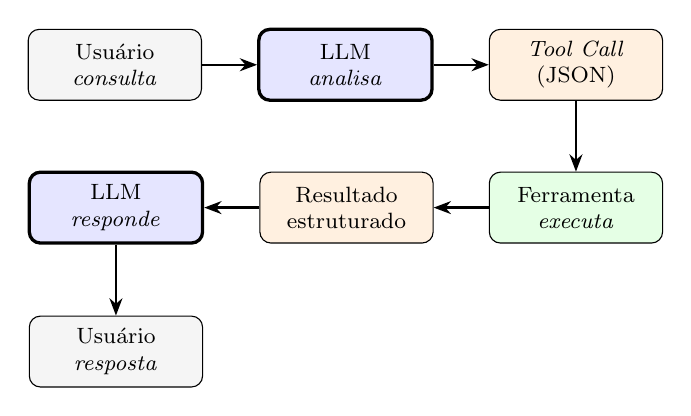
\begin{tikzpicture}[
  font=\footnotesize,
  node distance=0.9cm and 0.7cm,
  user/.style={rectangle, draw, rounded corners, minimum height=0.9cm, minimum width=2.2cm, align=center, fill=gray!8},
  llm/.style={rectangle, draw, rounded corners, minimum height=0.9cm, minimum width=2.2cm, align=center, fill=blue!10, very thick},
  payload/.style={rectangle, draw, rounded corners, minimum height=0.9cm, minimum width=2.2cm, align=center, fill=orange!12},
  tool/.style={rectangle, draw, rounded corners, minimum height=0.9cm, minimum width=2.2cm, align=center, fill=green!10},
  arr/.style={-{Stealth[length=2.2mm]}, thick}
]
  \node[user] (user1) {Usuário\\\textit{consulta}};
  \node[llm, right=of user1] (llm1) {LLM\\\textit{analisa}};
  \node[payload, right=of llm1] (call) {\textit{Tool Call}\\(JSON)};
  \node[tool, below=of call] (exec) {Ferramenta\\\textit{executa}};
  \node[payload, left=of exec] (result) {Resultado\\estruturado};
  \node[llm, left=of result] (llm2) {LLM\\\textit{responde}};
  \node[user, below=of llm2] (user2) {Usuário\\\textit{resposta}};

  \draw[arr] (user1) -- (llm1);
  \draw[arr] (llm1) -- (call);
  \draw[arr] (call) -- (exec);
  \draw[arr] (exec) -- (result);
  \draw[arr] (result) -- (llm2);
  \draw[arr] (llm2) -- (user2);
\end{tikzpicture}
\caption{Fluxo do mecanismo de \textit{Tool Calling}}
\label{fig:fluxo_toolcalling}
\fonte{Elaborado pelos autores.}
\end{figure}

No protocolo adotado pelo Ollama e pelo LangChain, cada ferramenta é definida por um \textit{schema} JSON com o nome da função, a sua descrição e os parâmetros aceitos, cada um com tipo e descrição. O modelo recebe essas definições junto com o \textit{prompt} de sistema, as instruções fixas que a aplicação lhe envia. A Figura~\ref{fig:exemplo_tool_schema} mostra uma definição simplificada da ferramenta de busca, com quatro dos doze parâmetros listados na Seção~\ref{sec:prototipo}.

\begin{figure}[h]
\centering
\begin{verbatim}
{
  "name": "buscar_catalogo",
  "description": "Busca produtos cartograficos no catalogo",
  "parameters": {
    "type": "object",
    "properties": {
      "keyword": {"type": "string",
                  "description": "Codigo MI, INOM ou nome da carta"},
      "scale":   {"type": "string",
                  "enum": ["1:25.000", "1:50.000", "1:100.000", ...],
                  "description": "Escala cartografica"},
      "state":   {"type": "string",
                  "description": "Nome do estado (normalizado)"},
      "productType": {"type": "string",
                       "description": "Tipo de produto SCN"}
    }
  }
}
\end{verbatim}
\caption{Exemplo simplificado de definição de ferramenta para busca em catálogo de produtos cartográficos}
\label{fig:exemplo_tool_schema}
\fonte{Elaborado pelos autores.}
\end{figure}

\subsection{\textit{Tool Calling} \textit{versus} Saída Estruturada}
\label{sec:tc-vs-se}

Na Saída Estruturada (\textit{Structured Output}), o modelo devolve a resposta num objeto JSON que segue um \textit{schema} predefinido, validado por bibliotecas como o Pydantic, em Python \cite{pydantic2019}, ou o Zod, em TypeScript. O modelo só decide quais campos preencher e com que valores. Bibliotecas como o Instructor \cite{instructor2023} conferem a saída contra o \textit{schema} e repetem a chamada quando ela é inválida.

A Saída Estruturada tem duas limitações estruturais. A primeira é que ela sempre devolve um objeto no formato do \textit{schema}. Mesmo com campos opcionais, toda consulta vira uma busca, e recusar exige um artifício no próprio \textit{schema}, como um campo de recusa. A segunda é que o modelo não consulta ferramentas durante a resposta. Uma verificação só lhe chega como nova tentativa, depois de emitido o objeto inteiro, como no Instructor. É esse o arranjo do controle da v3 (Seção~\ref{sec:v3}). Há ainda o risco de alucinações estruturadas, valores plausíveis sem apoio na consulta, inseridos para completar o \textit{schema}, hipótese que a Seção~\ref{sec:abordagens} testa.

No \textit{Tool Calling}, o modelo decide se e quando chama cada uma das ferramentas disponíveis. Ele pode responder sem chamar nenhuma ou encadear várias chamadas. Para este trabalho, o \textit{Tool Calling} pode ser mais adequado, porque deixa o modelo tratar consultas ambíguas, escolher os parâmetros relevantes e encadear validações antes da busca. Essa vantagem só se estabelece empiricamente. O Capítulo~\ref{cap:resultados} compara as duas abordagens numa só chamada (Seção~\ref{sec:abordagens}), na v3, em que as duas recebem o validador e só o \textit{Tool Calling} recebe as ferramentas auxiliares (Seção~\ref{sec:v3-resultados}), e no teste A/B, em acurácia e em tempo de processamento (Seção~\ref{sec:ab}).

% ---
\section{Modelos de Linguagem de Grande Porte e Execução Local}
% ---

Os LLMs, baseados na arquitetura \textit{Transformer} \cite{vaswani2017attention}, geram a resposta um \textit{token} (fragmento de palavra) por vez, condicionados ao \textit{prompt} de sistema, à consulta e ao que já geraram. O porte do modelo é o número de pesos, os parâmetros numéricos aprendidos no treinamento, contado em bilhões (B), como no Qwen 3 4B. A propriedade que mais importa aqui é seguir instruções em linguagem natural (\textit{instruction following}), obtida pelo ajuste fino com instruções e com \textit{feedback} humano \cite{ouyang2022training}. O \textit{Tool Calling} depende dela, porque o modelo precisa entender a consulta, interpretar o \textit{schema} das ferramentas e decidir como preenchê-lo.

\subsection{Vantagens e Desvantagens da Execução Local}

Executar os LLMs localmente, em vez de usar APIs de serviços em nuvem, traz vantagens para instituições como a DSG \cite{ollama2023}. As consultas e os dados não trafegam por redes externas, o que pesa em organizações com restrições de sigilo. Não há custo recorrente por \textit{token}. A organização mantém a versão exata do modelo em uso, o que permite auditá-lo. O sistema funciona sem conexão com a Internet.

A execução local tem também desvantagens:
\begin{itemize}
\item \textbf{Acesso limitado aos modelos de fronteira}. Os LLMs proprietários mais capazes não têm os pesos publicados e ocupam a maior parte das primeiras posições em \textit{benchmarks} de chamada de funções, como o \textit{Berkeley Function Calling Leaderboard} (BFCL) \cite{patil2025berkeley}.
\item \textbf{Custo de infraestrutura}. O gasto passa do pagamento por uso para o \textit{hardware}. A organização precisa adquirir e manter servidores com GPU e VRAM suficientes e arcar com energia, refrigeração e atualização de \textit{drivers}.
\item \textbf{Ciclo de atualização interno}. Cada nova versão de modelo exige repetir a avaliação sistemática.
\end{itemize}

\subsection{Ollama e Modelos com Suporte a \textit{Tool Calling}}

O Ollama \cite{ollama2023} é uma plataforma de código aberto que instala, executa e gerencia modelos de linguagem localmente. Ele expõe uma API compatível com o padrão OpenAI, o que facilita a integração com \textit{frameworks} como o LangChain. Para gerar as respostas, usa o \texttt{llama.cpp}, com os modelos no formato GGUF \cite{gguf2023}. O formato comporta quantizações como Q4\_0 e Q4\_K\_M, que reduzem a precisão dos pesos de 16 para cerca de 4 bits com perda pequena de qualidade, como mostram métodos de quantização pós-treinamento em 4 bits \cite{frantar2022gptq}. Este trabalho usou quantizações de 4 bits, Q4\_K\_M ou a equivalente da \textit{build} publicada de cada modelo (Seção~\ref{sec:selecao-modelos}), o que divide por cerca de quatro a memória de vídeo ocupada pelos pesos. Como ordem de grandeza, os pesos em 4 bits ocupam cerca de 0,5~GB por bilhão de parâmetros, e a memória do contexto, que cresce com o texto processado, se soma a eles.

A Tabela~\ref{tab:modelos_toolcalling} lista os quatro modelos avaliados (Seção~\ref{sec:selecao-modelos}). Os tamanhos orientaram a escolha de modelos executáveis na estação de referência, com GPU de 4~GB de VRAM, em que nenhum dos quatro coube inteiro. O excedente roda na CPU (\textit{offload}), o que aumenta a latência (Seção~\ref{sec:ambiente}).

\begin{table}[h]
\centering
\caption{Modelos avaliados, com suporte a \textit{Tool Calling} no Ollama}
\label{tab:modelos_toolcalling}
\resizebox{\textwidth}{!}{%
\begin{tabular}{|l|c|c|l|}
\hline
\textbf{Modelo} & \textbf{Parâmetros} & \textbf{Tamanho aprox. (4 bits)} & \textbf{Organização} \\
\hline
Gemma 4 E2B          & 2B efet.      & $\sim$4 GB$^{a}$ & Google DeepMind \\
Gemma 4 E4B          & 4B efet.      & $\sim$5{,}7 GB$^{a}$ & Google DeepMind \\
Qwen 3 4B            & 4B            & $\sim$2{,}3 GB & Alibaba Cloud \\
Mistral Nemo 12B     & 12B           & $\sim$6{,}6 GB  & Mistral AI e NVIDIA \\
\hline
\end{tabular}%
}
\fonte{Compilado pelos autores a partir de \citeauthoronline{ollama2023} (\citeyear{ollama2023}) e da documentação oficial dos modelos.}
\nota{$^{a}$~Tamanho da \textit{build} com quantização consciente de treinamento (QAT, 4 bits) publicada no Ollama (\texttt{gemma4:e2b-it-qat} e \texttt{gemma4:e4b-it-qat}). ``Efet.'' indica parâmetros efetivos; o total armazenado é maior (4,6B no E2B, segundo o Ollama), o que explica, em parte, o tamanho acima da ordem de grandeza de 0,5~GB por bilhão de parâmetros.}
\end{table}

% ---
\section{Orquestração com LangChain}
% ---

O LangChain \cite{langchain2022} é um \textit{framework} de código aberto para aplicações com LLMs, com uma interface comum para modelos, \textit{prompts} e ferramentas. Neste trabalho, ele liga a ferramenta de busca ao modelo, recolhe as chamadas de ferramenta que o modelo gera e é a interface única com os modelos no \textit{pipeline} de avaliação. Trocar a classe do Ollama (\texttt{ChatOllama}) pela de um provedor em nuvem (\texttt{ChatOpenAI} ou \texttt{ChatAnthropic}) exige alteração mínima no código, e a escolha entre execução local e em nuvem passa a ser uma decisão gerencial. O LangGraph \cite{langgraph2024}, extensão que modela fluxos como grafos de estados, não foi necessário. Na v1, a tradução é uma única decisão do modelo, e o laço da v3 é curto, tem limites fixos e é escrito explicitamente (Seções~\ref{sec:orquestracao} e~\ref{sec:v3}).

% ---
\section{Métricas de Avaliação}
\label{sec:metricas-conceitos}
% ---

As métricas servem para escolher o modelo e a abordagem a implantar, diante do compromisso entre qualidade e latência, e para reavaliar a solução quando surgirem modelos novos, o que o \textit{pipeline} de avaliação permite a custo baixo (Seção~\ref{sec:pipeline-avaliacao}). As métricas adotadas vêm da literatura de recuperação de informação \cite{manning2008introductionir}. Elas medem a correção total, a correção por campo e o tempo. A acurácia é o critério principal, e as demais desempatam ou medem o custo (Seção~\ref{sec:criterios-decisao}). A comparação com o gabarito é feita campo a campo, e não byte a byte, com as regras de normalização da Seção~\ref{sec:metricas}.

A \textbf{acurácia} é a proporção de consultas em que o modelo extraiu corretamente todos os parâmetros esperados, sem acrescentar parâmetros ausentes do gabarito. Nas consultas em que o gabarito prevê não buscar, a resposta é correta quando o modelo não chama a ferramenta de busca.
\[
\text{Acurácia} = \frac{\text{Número de consultas completamente corretas}}{\text{Total de consultas}}.
\]
É a métrica mais estrita, porque qualquer erro em qualquer parâmetro torna a consulta incorreta.

A análise por campo usa a \textbf{precisão}, o \textbf{\textit{recall}} e o \textbf{F1-\textit{score}},
\[
\text{Precisão} = \frac{\mathit{TP}}{\mathit{TP} + \mathit{FP}}
\qquad
\text{Recall} = \frac{\mathit{TP}}{\mathit{TP} + \mathit{FN}}
\qquad
F_1 = 2 \cdot \frac{\text{Precisão} \times \text{Recall}}{\text{Precisão} + \text{Recall}},
\]
em que $\mathit{TP}$ (\textit{true positives}) são os campos com valor aceito, $\mathit{FP}$ (\textit{false positives}) os campos com valor errado ou que não deviam ser emitidos e $\mathit{FN}$ (\textit{false negatives}) os campos obrigatórios omitidos. A decisão de recusar uma consulta é avaliada com as mesmas medidas, como uma classificação (Seção~\ref{sec:metricas}).

A \textbf{latência} é o tempo da tradução, do envio da consulta ao modelo até a decisão final de busca, numa ou em várias chamadas ao modelo. Ela é reportada por ambiente de execução, com estatísticas da sua distribuição sobre as consultas (Seção~\ref{sec:metricas}).

% ---
\section{Trabalhos Relacionados}
\label{sec:trabalhos-relacionados}
% ---

O ponto de partida direto deste trabalho, o protótipo do 1º CGEO \cite{cgeo2025prototipo}, é analisado na Seção~\ref{sec:prototipo}.

\paragraph{Interfaces de linguagem natural para bancos de dados.} Na formulação \textit{text-to-SQL}, o modelo gera a consulta SQL completa a partir da pergunta e do esquema do banco. O \textit{dataset} Spider \cite{yu2018spider} consolidou essa avaliação, com cerca de dez mil perguntas sobre 200 bancos. Com os LLMs, a abordagem passou a depender sobretudo do \textit{prompt}, e a ambiguidade e a subespecificação da linguagem natural estão entre os problemas centrais apontados pela literatura \cite{liu2025survey}. Neste trabalho, a formulação é mais restrita. O modelo não escreve SQL nem vê o esquema do banco. Ele só preenche os parâmetros tipados de uma ferramenta fixa, e o \textit{backend} monta com esses valores uma consulta SQL parametrizada. A restrição elimina o risco de SQL inválido ou injetado pelo modelo e permite validar cada argumento contra os enumerados do domínio. O custo é atender só às buscas que a ferramenta representa.

\paragraph{LLMs em geoinformação.} \citeonline{mai2023geospatialllm} discutem as oportunidades e os desafios dos modelos de fundação para a inteligência artificial geoespacial, e \citeonline{manvi2024geollm} mostram que o conhecimento geográfico dos LLMs serve a tarefas de predição quando o \textit{prompt} traz contexto do OpenStreetMap. Os LLMs passaram também a comandar tarefas de Sistemas de Informação Geográfica (SIG). O LLM-Geo, SIG autônomo construído por \citeonline{li2023autonomous} sobre o GPT-4, gera e executa o código que coleta, analisa e visualiza dados espaciais, e o GeoGPT \cite{zhang2024geogpt} planeja e encadeia ferramentas de SIG a partir de pedidos em linguagem natural. Nesses sistemas, o modelo tem alta autonomia. Neste trabalho, o modelo, aberto e executado localmente, só decide se busca e com quais argumentos, numa chamada na v1 e num laço curto com ferramentas auxiliares e um validador na v3, sempre com uma única ferramenta de busca.

\paragraph{Descoberta de dados geoespaciais.} A dificuldade de encontrar dados em geoportais é anterior aos LLMs. \citeonline{hu2015metadata} a atribuem, em parte, à heterogeneidade dos metadados e propõem harmonização de tópicos e busca semântica em geoportais baseados em \textit{Linked Data}. Com os LLMs, \citeonline{ning2025autonomous} propõem um agente que escolhe a fonte de dados numa lista predefinida e gera o programa que a recupera, e \citeonline{li2025question} combinam LLMs e um grafo de conhecimento construído a partir de cinco grandes portais para responder a perguntas de descoberta de dados. No caso da DSG, o catálogo é único e já estruturado, e o problema se reduz a traduzir a intenção do usuário nos filtros desse catálogo. Por isso a solução dispensa grafo de conhecimento e geração de código.

\paragraph{Avaliação da chamada de ferramentas.} Os trabalhos sobre uso de ferramentas por LLMs trouxeram \textit{benchmarks} próprios, como o API-Bank \cite{li2023apibank}, o ToolBench do ToolLLM \cite{qin2023toolllm}, com mais de 16 mil APIs reais, e o APIBench do Gorilla \cite{patil2023gorilla}. O BFCL \cite{patil2025berkeley} compara a chamada gerada com a esperada pela árvore sintática e avalia também a abstenção. Segundo ele, os melhores modelos vão bem em chamadas de um único turno, mas ainda não em memória, decisões dinâmicas e raciocínio de longo prazo. Esses \textit{benchmarks}, na maioria em inglês, de domínio geral e com muitas ferramentas, não cobrem o cenário deste trabalho, que reúne uma única ferramenta de busca, consultas em português com o vocabulário da cartografia sistemática (MI, INOM, escalas, centros produtores) e modelos pequenos executados localmente. Por isso este trabalho construiu um \textit{dataset} próprio, com gabarito auditado e comparação campo a campo semelhante, em espírito, à comparação estrutural do BFCL.

\paragraph{Ferramentas auxiliares e retorno.} No ReAct \cite{yao2023react}, o modelo alterna raciocínio e ações, e o resultado de cada ação alimenta o passo seguinte. A correção funciona quando o sinal vem de fora do modelo. O CRITIC \cite{gou2024critic} verifica a saída com ferramentas e a revisa, e o \textit{self-debugging} \cite{chen2024selfdebug} corrige consultas a partir do resultado da execução. A autocorreção sem sinal externo \cite{madaan2023selfrefine} pode não ajudar e até piorar o raciocínio \cite{huang2024cannot}. O ToolSandbox \cite{lu2025toolsandbox} aponta a normalização de argumentos, como datas relativas e lugares, entre as maiores dificuldades. O When2Call \cite{ross2025when2call} mostra que decidir entre chamar, perguntar ou recusar é uma capacidade própria, fraca em modelos pequenos. O $\tau$-bench \cite{yao2025taubench} avalia diálogos com usuário simulado, e o CRITICTOOL \cite{huang2025critictool} classifica os erros de chamada que o modelo precisa perceber e corrigir.

Ajustar um sistema pelos erros de um conjunto rotulado arrisca torná-lo bom só nesse conjunto (sobreajuste). O risco vale para as lições que o modelo acumula a partir de sucessos e falhas, como no Reflexion \cite{shinn2023reflexion} e no ExpeL \cite{zhao2024expel}, e para a otimização automática de \textit{prompts} \cite{yang2024opro,khattab2024dspy}. Medir o resultado exige um conjunto de teste que o desenvolvimento não tenha visto \cite{dwork2015reusable}. A v3 (Seção~\ref{sec:v3}) leva a um domínio restrito as ferramentas auxiliares determinísticas, a validação com retorno e o pedido de esclarecimento a um usuário simulado, acrescentados em degraus, e foi testada num lote que o desenvolvimento não leu.

% ----------------------------------------------------------
% Capítulo 3 — Metodologia
% ----------------------------------------------------------
\chapter{Metodologia}
\label{cap:metodologia}

Este capítulo descreve o método de trabalho adotado para o aprimoramento da solução de busca em linguagem natural sobre o acervo cartográfico da DSG. O trabalho parte de um protótipo de referência desenvolvido pelo 1º CGEO, descrito e analisado em detalhe no Capítulo~\ref{cap:aprimoramento}, e adota a estratégia de \textbf{substituição dirigida}: identificam-se os componentes responsáveis pelas limitações documentadas pelo cliente e substituem-se esses componentes por equivalentes mais robustos, preservando o que já funciona (esquema do banco, conjunto de parâmetros de busca, lógica das consultas espaciais).

O capítulo apresenta os elementos transversais ao projeto: o escopo (entregáveis e exclusões), os modelos comparados, a construção e a auditoria do \textit{dataset} de avaliação, os dois lotes de validação, as especificações v2 e v3 e o protocolo de medição. A execução do aprimoramento --- análise do protótipo, requisitos, planejamento da migração, desenvolvimento por camadas e cronograma --- é apresentada no Capítulo~\ref{cap:aprimoramento}.

\paragraph{Foco da avaliação: a camada de tradução linguística.} O objeto de avaliação deste trabalho é o desempenho do LLM na \textbf{tradução de uma consulta em linguagem natural para os parâmetros estruturados} de busca no catálogo. A execução dessa consulta contra o banco (PostgreSQL/PostGIS), a resolução de nomes geográficos e a interpretação das \textit{bounding boxes} das cartas são componentes herdados do protótipo do 1º CGEO; sua correção é assumida como \textit{caixa-preta} e não é medida. Métricas sobre o \textit{conjunto de produtos retornados} ficam fora do escopo (Seção~\ref{sec:exclusoes-avaliacao}) e são apontadas como direção de trabalho futuro no Capítulo~\ref{cap:conclusao}. O LLM é comparado contra um \textit{ground truth} de \textbf{parâmetros extraídos}, não de produtos recuperados.

% ---
\section{Escopo do Projeto}
% ---

\subsection{Entregáveis}

O projeto entregou:

\begin{itemize}
  \item uma nova arquitetura de \textit{backend} em Python (FastAPI + LangChain), que substitui o \textit{backend} Node.js do protótipo e implementa \textit{Tool Calling} nativo via Ollama;
  \item um \textit{dataset} de avaliação com 310 consultas de referência (\textit{ground truth}), distribuídas em seis categorias de consulta e uma de consultas fora do domínio, acompanhado de um manual de anotação e de um relatório de auditoria;
  \item um \textit{pipeline} de avaliação automatizado, que executa o \textit{dataset} sobre cada modelo e produz as métricas de acurácia, precisão, \textit{recall}, F1-\textit{score} e latência, com os testes estatísticos correspondentes;
  \item um relatório comparativo entre quatro modelos de LLM com suporte a \textit{Tool Calling}, executados localmente, com a recomendação fundamentada do modelo mais adequado para uso operacional sobre o acervo da DSG, complementado por uma referência paralela com modelos maiores servidos em nuvem;
  \item dois lotes de validação independentes (Seções~\ref{sec:lote-validacao} e~\ref{sec:v3}) e a v3 do \textit{Tool Calling}, com ferramentas auxiliares e validação com retorno, desenvolvida sobre as 310 consultas e o primeiro lote e testada no segundo contra um controle com Saída Estruturada; a v3 está implementada no pacote e no avaliador (\texttt{src/pfc\_busca/v3.py}), mas ainda não integrada à API do \textit{backend}.
\end{itemize}

\subsection{Exclusões}
\label{sec:exclusoes-avaliacao}

Estão fora do escopo deste trabalho:

\begin{itemize}
  \item \textbf{Avaliação da qualidade de recuperação em nível de produto}: uma vez extraídos os parâmetros, o conjunto de produtos retornado depende do motor de busca (\texttt{buscar\_catalogo}) e da qualidade do banco cartográfico, ambos herdados do protótipo. O trabalho \textbf{não mede} precisão e \textit{recall} em nível de produto. A execução SQL permanece no \textit{pipeline} apenas como demonstração de que a arquitetura fecha ponta a ponta;
  \item \textbf{Resolução avançada de nomes geográficos}: o cruzamento entre \textit{strings} livres (estado, município) e as \textit{bounding boxes} das cartas depende de recursos externos (malha do IBGE, Nominatim/OSM) e da qualidade das geometrias no banco; é tratado como trabalho futuro (Capítulo~\ref{cap:conclusao});
  \item desenvolvimento de interface gráfica (\textit{frontend}) para o usuário final;
  \item implantação em produção em ambiente da DSG ou de suas OM subordinadas;
  \item pesquisa de opinião ou avaliação qualitativa com usuários;
  \item treinamento ou ajuste fino (\textit{fine-tuning}) de modelos de linguagem;
  \item busca por coordenadas geográficas brutas (\textit{bounding box}) sem referência nominal a um lugar;
  \item suporte a idiomas além do português brasileiro.
\end{itemize}

\subsection{Requisitos que norteiam o escopo}
\label{sec:requisitos-resumo}

O escopo é norteado por requisitos funcionais (RF) e não funcionais (RNF) elicitados a partir da análise do protótipo e das conversas com o cliente. O Quadro~\ref{quadro:requisitos-resumo} traz o resumo; a discussão completa está no Capítulo~\ref{cap:aprimoramento} (Seção~\ref{sec:requisitos}).

\begin{quadro}[h]
\centering
\caption{Resumo dos requisitos que norteiam o escopo}
\label{quadro:requisitos-resumo}
\small
\begin{tabular}{|c|p{5.5cm}|c|p{5.0cm}|}
\hline
\multicolumn{2}{|l|}{\textbf{Requisitos Funcionais (RF)}} & \multicolumn{2}{l|}{\textbf{Requisitos N\~ao Funcionais (RNF)}} \\
\hline
RF1 & Receber consulta em linguagem natural via REST & RNF1 & Execu\c c\~ao totalmente local (privacidade) \\
\hline
RF2 & Traduzir consulta em par\^ametros do \textit{schema} & RNF2 & Lat\^encia mediana operacional aceit\'avel \\
\hline
RF3 & Executar busca no PostgreSQL/PostGIS & RNF3 & Conformidade a ET-PCDG e Perfil MGB \\
\hline
RF4 & Selecionar modelo por requisi\c c\~ao (\textit{dev only}) & RNF4 & Reprodutibilidade dos experimentos \\
\hline
RF5 & Registrar tra\c cos para as m\'etricas & RNF5 & Manutenibilidade (m\'odulos, testes) \\
\hline
    &                                       & RNF6 & Substituibilidade de modelo por configura\c c\~ao \\
\hline
\end{tabular}%
\fonte{Elaborado pelos autores. Detalhes no Cap.~\ref{cap:aprimoramento}, Seção~\ref{sec:requisitos}.}
\end{quadro}

Requisitos ideais são mensuráveis, mas alguns dos RNF --- em particular o RNF2, latência --- dependem de fatores externos ao escopo deste PFC (\textit{hardware} do ambiente de implantação, carga concorrente). Por isso os valores de latência são reportados nas condições de cada ambiente de execução (Seção~\ref{sec:ambiente}), sem limiar operacional fixado \textit{a priori}.

% ---
\section{Seleção de Modelos}
\label{sec:selecao-modelos}
% ---

\subsection{Critérios de Seleção}

Os modelos foram selecionados segundo os critérios: (i) disponibilidade no Ollama com suporte nativo a \textit{Tool Calling}, verificada no catálogo oficial da biblioteca~\cite{ollama2023}, que mantém rankings de popularidade e uma etiqueta explícita de compatibilidade com \textit{tool calling}; (ii) disponibilidade em versões quantizadas compatíveis com estações de trabalho modestas; (iii) lançamento ou atualização entre 2024 e 2026; e (iv) diversidade de arquiteturas e organizações desenvolvedoras.

\subsection{Modelos Avaliados}

Foram avaliados quatro modelos abertos, executados localmente pelo Ollama:

\begin{enumerate}
  \item \textbf{Qwen 3 4B}~\cite{qwen2025qwen3} (Alibaba Cloud), \textit{tag} \texttt{qwen3:4b-instruct-\allowbreak 2507-q4\_K\_M}: 4 bilhões de parâmetros, quantização Q4\_K\_M, 2,3~GB --- a menor \textit{build} dos quatro; mesmo assim, carregado com o contexto, não coube inteiro nos 4~GB de VRAM da estação de referência, onde o Ollama alocou na GPU \res{estacao}{qwen}{nagpu} do modelo carregado (Tabela~\ref{tab:ambiente_estacao}). Usou-se a \textit{build} oficial sem raciocínio interno (\textit{Instruct-2507}), pela razão explicada na Seção~\ref{sec:config-modelos};
  \item \textbf{Gemma 4 E4B}~\cite{team2026gemma4} (Google DeepMind), \textit{tag} \texttt{gemma4:\allowbreak e4b-it-qat}: variante \textit{edge} de cerca de 4 bilhões de parâmetros efetivos, com quantização consciente de treinamento. É a menor \textit{build} publicada do E4B ($\sim$5,7~GB) e não cabe em 4~GB de VRAM --- a variante Q4\_K\_M ocupa $\sim$9~GB ---, o que exige \textit{offload} parcial para a CPU na estação de referência;
  \item \textbf{Gemma 4 E2B}~\cite{team2026gemma4}, \textit{tag} \texttt{gemma4:\allowbreak e2b-it-qat}: variante menor da mesma família, com cerca de 2 bilhões de parâmetros efetivos ($\sim$4,0~GB), incluída como alternativa de menor custo computacional ao E4B, que não cabe na VRAM da estação de referência; o E2B também recebe \textit{offload} parcial nessa estação. Permite observar, dentro de uma mesma família, o efeito do tamanho do modelo;
  \item \textbf{Mistral Nemo 12B}~\cite{mistral2024nemo} (Mistral AI e NVIDIA), \textit{tag} \texttt{mistral-nemo:\allowbreak 12b}: 12 bilhões de parâmetros ($\sim$6,6~GB), com suporte consolidado a \textit{Tool Calling} e bom desempenho em português. Representa a faixa superior de tamanho executável com \textit{offload} parcial numa estação modesta.
\end{enumerate}

\subsection{Referência paralela em nuvem}

Como referência --- e não como candidatos à implantação, uma vez que o requisito RNF1 exige execução local ---, a mesma avaliação foi executada sobre \res{groq}{geral}{nmodelos} modelos maiores servidos pelo provedor Groq e disponíveis com suporte a \textit{Tool Calling} em setembro de 2026: \res{groq}{geral}{tags} \cite{qwen2026qwen38, openai2025gptoss}. Os três têm pesos abertos, sob licença Apache 2.0, mas exigem mais memória do que a estação de referência oferece. O objetivo é situar os modelos locais em relação a modelos de maior porte sob o mesmo \textit{prompt}, a mesma ferramenta, o mesmo \textit{dataset} e as mesmas métricas. A troca de provedor usa exatamente a portabilidade descrita no Capítulo~\ref{cap:referencial}: o \texttt{ChatOllama} do LangChain é substituído pelo \texttt{ChatOpenAI} apontado para o \textit{endpoint} compatível do provedor, sem alteração no restante do \textit{pipeline}. Esses resultados são sempre reportados à parte e identificados como execução em nuvem.

% ---
\section{Construção do \textit{Dataset} de Avaliação}
\label{sec:dataset}
% ---

A comparação objetiva dos modelos exige um \textit{dataset} de referência representativo do espectro de consultas que usuários do catálogo tenderiam a formular, cobrindo diferentes níveis de complexidade e combinações de parâmetros, e cujo gabarito seja \textbf{auditável}: cada resposta esperada deve poder ser justificada a partir do texto da consulta e de regras escritas, e qualquer leitor deve poder refazer essa verificação.

O \textit{dataset} serve exclusivamente para \textbf{avaliação}: nenhum modelo foi treinado ou ajustado com ele, e cada modelo recebe as consultas uma a uma, sem exemplos resolvidos (\textit{zero-shot}). A qualidade que importa é, portanto, a do gabarito --- se cada resposta esperada está certa e se as leituras aceitas são todas as leituras legítimas da consulta ---, e ela se apoia em três mecanismos: regras de anotação escritas antes da anotação (Seção~\ref{sec:manual-anotacao}), construção rastreável em camadas (Seção~\ref{sec:camadas}) e uma auditoria com checagens automáticas, anotação independente às cegas, adjudicação registrada e conferência humana de uma amostra (Seção~\ref{sec:auditoria}).

\subsection{Estrutura de cada entrada}

Cada consulta do \textit{dataset} é registrada com os campos da Tabela~\ref{tab:estrutura-dataset}, acrescidos de \texttt{origem} (P, N ou G), \texttt{familia} (P, N, GS \ldots GF) e \texttt{trocas} (leituras estruturais alternativas, das quais \texttt{alternativas} é a expansão); valores alternativos e campos opcionais ficam marcados no próprio \texttt{esperado}. O arquivo \texttt{dataset.json} e o Apêndice~\ref{apendice:dataset} são gerados a partir da mesma fonte, de modo que não podem divergir.

\begin{table}[htbp!]
\centering
\caption{Estrutura de cada entrada do \textit{dataset} de avaliação}
\label{tab:estrutura-dataset}
\small
\begin{tabular}{|l|p{10.5cm}|}
\hline
\textbf{Campo} & \textbf{Descrição} \\
\hline
\texttt{id} & Identificador (P01--P22, N01--N40, GS001 \ldots GF007) \\ \hline
\texttt{fonte} & Rastreabilidade: arquivo e linha de origem (camada P), autores (camada N) ou função geradora, modelo de frase e semente (camada G) \\ \hline
\texttt{categorias} & Uma ou mais das categorias S, C, M, T, O, A; ou F (fora do domínio), que não se combina com as demais \\ \hline
\texttt{consulta} & Texto em linguagem natural \\ \hline
\texttt{esperado} & Leitura preferencial do gabarito: parâmetros de busca na forma canônica, com períodos relativos expressos por regras nomeadas \\ \hline
\texttt{alternativas} & Demais leituras aceitas, quando a consulta admite mais de uma (Seção~\ref{sec:manual-anotacao}) \\ \hline
\texttt{espera\_tool\_call} & Falso quando o comportamento correto é não chamar a ferramenta \\ \hline
\texttt{observacional} & Verdadeiro quando o caso fica fora das métricas principais \\ \hline
\texttt{notas} & Justificativa das leituras alternativas e observações do anotador \\ \hline
\end{tabular}%
\fonte{Elaborada pelos autores.}
\end{table}

\subsection{Categorias de Consultas}

O \textit{dataset} é organizado em seis categorias, alinhadas aos exemplos do protótipo e às demandas do cliente: \textbf{simples} (S, um único parâmetro: ``cartas de São Paulo''); \textbf{compostas} (C, dois ou mais parâmetros: ``ortoimagens de Manaus em 1:50.000''); \textbf{com código MI/INOM} (M: ``INOM SG-22-X-A''); \textbf{com referência temporal relativa} (T: ``nos últimos 3 meses'', ``depois de 2022''); \textbf{com ordenação} (O: ``as 3 cartas mais antigas''); e \textbf{ambíguas ou informais} (A: siglas, grafias sem acento, abreviações e expressões qualitativas). Uma consulta pode pertencer a mais de uma categoria. Uma sétima categoria, \textbf{fora do domínio} (F: ``cartas de Marte'', ``qual a previsão do tempo para amanhã em Manaus?''), reúne as consultas em que a resposta correta é não chamar a ferramenta; ela mede a capacidade de o modelo recusar pedidos que o catálogo não atende.

\subsection{Camadas de Construção}
\label{sec:camadas}

O \textit{dataset} tem 310 consultas, construídas em três camadas complementares (Tabela~\ref{tab:dataset-composicao}):

\begin{enumerate}
  \item \textbf{Camada P (protótipo, 22 casos)}: as consultas do arquivo de testes do protótipo (\texttt{backend/\allowbreak evaluation/\allowbreak test-cases.ts}), cada uma rastreada até a linha de origem. A anotação original da equipe do 1º CGEO é mantida como leitura preferencial --- o \textit{baseline} não é reanotado ---, e as leituras alternativas acrescentadas seguem o manual de anotação, com justificativa registrada. Os gabaritos de datas relativas do arquivo original, calculados para uma data de referência do início de 2025, são substituídos pelas regras nomeadas da Seção~\ref{sec:manual-anotacao}, que se resolvem na data de referência de cada rodada.
  \item \textbf{Camada N (autores, 40 casos)}: redigidos para preencher lacunas de distribuição --- em especial a categoria Simples, ausente na camada P --- e para exercitar ambiguidades e casos de fronteira do domínio.
  \item \textbf{Camada G (geração programática, 248 casos)}: consultas sintetizadas pela combinação de catálogos fechados do domínio --- 27 UFs, 12 municípios de referência, 8 escalas do SCN, 9 tipos de produto das ET-PCDG, 5 CGEOs, 9 projetos, códigos MI e INOM, 15 expressões de tempo (14 relativas e o intervalo absoluto ``entre 2022 e 2023'') e padrões de ordenação --- em modelos de frase do português corrente (com preposição adequada a cada UF e apelidos usuais de escala, como ``25k'' ou ``escala de 25 mil''). O gabarito é conhecido \textbf{por construção}: a frase é montada a partir dos parâmetros que deve produzir. A geração é determinística (semente 42) e rejeita, dentro da camada G, qualquer consulta que repita outra após normalização; a construção do \textit{dataset} verifica ainda que nenhuma consulta gerada repita, após normalização, uma das camadas P e N, e é interrompida se isso ocorrer. A camada inclui sete consultas de fronteira do domínio (família G-F): seis fora do domínio e uma observacional.
\end{enumerate}

\begin{table}[htbp!]
\centering
\caption{Composição do \textit{dataset} de avaliação por origem e família}
\label{tab:dataset-composicao}
\small
\begin{tabular}{|l|>{\centering\arraybackslash}p{1.9cm}|>{\centering\arraybackslash}p{2.3cm}|>{\centering\arraybackslash}p{2.9cm}|}
\hline
\textbf{Origem / família} & \textbf{Consultas} & \textbf{Observa\-cionais} & \textbf{Com mais de uma leitura aceita} \\
\hline
Protótipo do 1º CGEO (P) & 22 & 0 & 11 \\
Autores (N) & 40 & 3 & 15 \\
Geradas --- simples (G-S) & 61 & 0 & 0 \\
Geradas --- compostas (G-C) & 55 & 0 & 3 \\
Geradas --- código MI/INOM (G-M) & 28 & 0 & 0 \\
Geradas --- tempo relativo (G-T) & 41 & 0 & 20 \\
Geradas --- ordenação (G-O) & 19 & 0 & 16 \\
Geradas --- informais (G-A) & 24 & 0 & 2 \\
Geradas --- amplas (G-P) & 13 & 0 & 0 \\
Geradas --- fronteira (G-F) & 7 & 1 & 0 \\
\hline
\textbf{Total} & \textbf{310} & \textbf{4} & \textbf{67} \\
\hline
\end{tabular}
\fonte{Elaborada pelo autor a partir de \texttt{dataset.json}.}
\end{table}


\paragraph{Justificativa da geração programática.} Consultas escritas à mão são caras de redigir e anotar e tendem a variar sobre um pequeno conjunto de padrões familiares aos autores. A geração por modelos de frase sobre catálogos fechados oferece cobertura sistemática de combinações raras (pares UF $\times$ escala pouco frequentes, por exemplo), escala sem custo adicional de anotação e volume suficiente para estimar intervalos de confiança e comparar modelos com testes de significância. A contrapartida é a regularidade linguística, que pode favorecer os modelos: por isso a acurácia é também desagregada por camada (Tabela~\ref{tab:resultados_por_origem}), o que permite distinguir o desempenho nas consultas geradas do desempenho nas consultas redigidas por pessoas (P e N).

\begin{table}[htbp!]
\centering
\caption{Consultas por categoria e por camada (métricas principais; uma consulta pode ter mais de uma categoria)}
\label{tab:dataset-categorias}
\small
\begin{tabular}{|l|c|c|c|c|}
\hline
\textbf{Categoria} & \textbf{P} & \textbf{N} & \textbf{G} & \textbf{Total} \\
\hline
Simples (S) & 0 & 11 & 89 & 100 \\
Compostas (C) & 22 & 21 & 137 & 180 \\
Código MI/INOM (M) & 10 & 5 & 42 & 57 \\
Tempo relativo (T) & 6 & 9 & 45 & 60 \\
Ordenação (O) & 4 & 6 & 19 & 29 \\
Ambíguas/informais (A) & 16 & 19 & 162 & 197 \\
Fora do domínio (F) & 0 & 2 & 6 & 8 \\
\hline
\end{tabular}
\fonte{Elaborada pelo autor.}
\end{table}


\subsection{Manual de Anotação e Leituras Múltiplas}
\label{sec:manual-anotacao}

O gabarito é construído segundo um manual de anotação escrito (Apêndice~\ref{apx:manual}) que fixa seis princípios --- evidência explícita no texto, forma canônica, leituras múltiplas explícitas, tratamento das consultas fora do domínio, consistência e casos observacionais --- e regras para cada um dos doze campos da ferramenta.

O princípio mais importante para a confiabilidade da avaliação é o das \textbf{leituras múltiplas explícitas}. Uma parte das consultas admite, legitimamente, mais de uma resposta correta: ``cartas de São Paulo'' pode referir-se ao estado ou à capital; ``produtos publicados nos últimos 3 meses'' pode significar noventa dias ou três meses de calendário; ``as cartas mais recentes'' pode ser ordenado pela data de publicação ou pela de criação, pois a consulta não diz qual. Um gabarito que escolhesse uma única leitura penalizaria como erro uma resposta razoável e mediria a coincidência com a preferência do anotador, não a qualidade da tradução. Nesses casos o gabarito lista \textbf{todas} as leituras aceitas, por três mecanismos: \emph{valor alternativo} (o campo aceita mais de um valor), \emph{campo opcional} (pode faltar sem erro, como \texttt{limit = 1} em ``a carta mais recente'') e \emph{leitura estrutural alternativa} (o mesmo trecho pode ocupar campos diferentes, como \texttt{state} ou \texttt{city}). As expressões de tempo relativo são registradas como regras nomeadas, resolvidas na data de referência da rodada --- registrada no manifesto e informada ao modelo no \textit{prompt} de sistema --- com as leituras aceitas do Quadro~\ref{quadro:tempo-relativo}.

A ambiguidade não é, porém, tratada com leniência genérica: toda leitura aceita está escrita no gabarito, justificada por uma regra do manual e visível no Apêndice~\ref{apendice:dataset}; fora delas, a comparação é estrita (Seção~\ref{sec:metricas}). Das 306 consultas das métricas principais, a Tabela~\ref{tab:dataset-composicao} indica quantas admitem mais de uma leitura.

\paragraph{Consultas fora do domínio e casos observacionais.} Oito consultas estão fora do domínio (N36, N37 e seis da família G-F): o comportamento correto é determinado --- não chamar a ferramenta --- e elas entram nas métricas principais, na categoria F. Quatro consultas são observacionais (N38, N39, N40 e GF007), porque o comportamento correto não é determinável a partir do texto: valor impossível de representar (``escala 1:10.000.000'', ``cartas do estado 42'') ou pedido de resposta discutível (``cartas topo no oceano atlântico'', ``cartas do futuro (ano 2050)''). Elas são executadas e o comportamento de cada modelo é reportado à parte; as métricas principais cobrem as 306 consultas restantes.

\begin{table}[htbp!]
\centering
\caption{Frequência de cada campo na leitura preferencial do gabarito (métricas principais)}
\label{tab:dataset-campos}
\small
\begin{tabular}{|l|c||l|c|}
\hline
\textbf{Campo} & \textbf{Ocorr.} & \textbf{Campo} & \textbf{Ocorr.} \\
\hline
\texttt{keyword} & 62 & \texttt{project} & 11 \\
\texttt{scale} & 84 & \texttt{publicationPeriod} & 51 \\
\texttt{productType} & 44 & \texttt{creationPeriod} & 10 \\
\texttt{state} & 130 & \texttt{sortField} & 29 \\
\texttt{city} & 27 & \texttt{sortDirection} & 29 \\
\texttt{supplyArea} & 40 & \texttt{limit} & 21 \\
\hline
\end{tabular}
\fonte{Elaborada pelos autores.}
\end{table}


% ---
\section{Auditoria do \textit{Dataset}}
\label{sec:auditoria}
% ---

A confiabilidade das métricas depende diretamente da confiabilidade do gabarito. Por isso o \textit{dataset} foi submetido a uma auditoria em três etapas, repetidas até não restar divergência sem decisão registrada. O procedimento, as ferramentas e os resultados completos estão no Apêndice~\ref{apx:auditoria} e no repositório (\texttt{data/auditoria/}).

\begin{enumerate}
  \item \textbf{Checagens automáticas} (\texttt{pfc-auditar}): unicidade de identificadores e de consultas (após normalização de caixa, acentos e pontuação); validade de todos os valores contra os enumerados da ferramenta; resolução de todas as regras de tempo relativo em datas diversas, inclusive anos bissextos e viradas de ano; rastreabilidade das consultas da camada P até a linha citada do arquivo de origem; um \textbf{anotador por regras}, que localiza na consulta o trecho que justifica cada campo do gabarito e aponta campo sem evidência, evidência sem campo e valor divergente; e uma verificação de \textbf{consistência} de convenções entre casos (a mesma expressão, a mesma anotação).
  \item \textbf{Anotação independente às cegas}: todas as 310 consultas foram anotadas novamente, a partir do zero, por um modelo de linguagem de propósito geral de grande porte (Claude Opus 5.5, da Anthropic), que não integra o conjunto de modelos avaliados. A anotação foi feita em dez lotes de 31 consultas, em sessões independentes, cada uma com acesso apenas ao manual de anotação, à definição da ferramenta, à data de referência e ao próprio lote --- sem acesso ao gabarito, ao gerador ou aos demais lotes. Para cada consulta, o anotador registrou a decisão (chamar a ferramenta, não chamar ou caso observacional), a leitura preferencial, as leituras alternativas previstas pelo manual e uma justificativa por referência às regras.
  \item \textbf{Adjudicação}: cada consulta com divergência em qualquer das medidas de concordância recebeu uma decisão registrada --- gabarito mantido, corrigido ou ampliado com leitura alternativa --- com justificativa por referência ao manual. O gabarito anterior a cada decisão fica registrado, de modo que a concordância anterior à adjudicação pode ser recalculada a partir do repositório.
\end{enumerate}

A concordância entre o gabarito e a anotação independente foi medida em rigor crescente (Tabela~\ref{tab:auditoria}): a decisão sobre chamar a ferramenta, com o kappa de Cohen~\cite{cohen1960coefficient,artstein2008intercoder}, que desconta a concordância esperada ao acaso; a compatibilidade das leituras nos dois sentidos (a leitura do anotador é aceita pelo gabarito e a leitura preferencial do gabarito é aceita pelo anotador); a identidade da leitura preferencial; a presença e o valor de cada campo; e a detecção de ambiguidade, isto é, se a consulta admite mais de uma leitura. A coluna ``antes da adjudicação'' mede a concordância propriamente dita; a coluna ``após'' mostra o que restou depois das decisões.

\begin{table}[htbp!]
\centering
\caption{Resultados da auditoria do \textit{dataset}}
\label{tab:auditoria}
\small
\begin{tabular}{|p{7.3cm}|c|c|}
\hline
\textbf{Verificação} & \textbf{Antes da adjudicação} & \textbf{Após} \\
\hline
\multicolumn{3}{|l|}{\textit{Checagens automáticas}} \\ \hline
Problemas estruturais (ids, duplicatas, enumerados, datas) & --- & 0 \\ \hline
Consultas da camada P conferidas na linha de origem & --- & 22/22 \\ \hline
Apontamentos do anotador por regras sem resolução & --- & 0 \\ \hline
Expressões com anotação inconsistente sem justificativa & --- & 0 \\ \hline
\multicolumn{3}{|l|}{\textit{Anotação independente às cegas (310 consultas)}} \\ \hline
Decisão (chamar / não chamar / observacional) & 302/310 (97,4\%) & 310/310 (100,0\%) \\
\quad kappa de Cohen & 0,658 & 1,000 \\ \hline
Leituras compatíveis nos dois sentidos & 300/310 (96,8\%) & 309/310 (99,7\%) \\ \hline
Leitura preferencial idêntica$^{a}$ & 294/298 (98,7\%) & 294/298 (98,7\%) \\ \hline
Presença de cada campo na leitura preferencial$^{a,b}$ (kappa) & 0,999 & 0,999 \\ \hline
Valor do campo, quando ambos o anotam$^{a}$ & 534/537 (99,4\%) & 534/537 (99,4\%) \\ \hline
Consulta com mais de uma leitura aceita$^{a}$ & 296/298 (99,3\%) & 297/298 (99,7\%) \\
\quad kappa de Cohen & 0,981 & 0,990 \\ \hline
Consultas com divergência em alguma medida, sem decisão registrada & 14 & 0 \\ \hline
\end{tabular}
\fonte{Elaborada pelo autor a partir de \texttt{data/auditoria/}. (a) Sobre as consultas em que gabarito e anotador pedem a chamada da ferramenta nas métricas principais. (b) Doze campos por consulta.}
\end{table}


As medidas de campo e de ambiguidade mostram concordância quase perfeita já antes da adjudicação. A principal divergência foi de classificação: o gabarito tratava como observacionais oito consultas fora do domínio cujo comportamento correto é determinado pelo próprio manual (não chamar a ferramenta). A decisão foi corrigir o gabarito e incluí-las nas métricas principais, na categoria F. As demais divergências foram uma leitura ampliada (N33, em que ``cartografia sistemática'' passou a admitir a leitura sem o campo \texttt{project}, pois a expressão não consta da descrição da ferramenta) e cinco divergências mantidas com justificativa, entre elas três escolhas de leitura preferencial dentro do mesmo conjunto de leituras aceitas, que não afetam a pontuação. O Quadro~\ref{quadro:adjudicacao} do Apêndice~\ref{apx:auditoria} lista essas 14 decisões e mais uma, originada nas checagens de consistência (P14, mantida), num total de 15 consultas adjudicadas.

Duas ressalvas delimitam o alcance da auditoria. O anotador por regras foi escrito pelos autores e, portanto, verifica evidência e consistência, mas não constitui uma anotação independente. A anotação às cegas é independente do gabarito, mas foi feita por um modelo de linguagem, e não por uma pessoa: ela identifica divergências com alta sensibilidade, e a decisão sobre cada uma é tomada na adjudicação, por referência ao manual. Na camada G, além disso, o gabarito é conhecido por construção, e a auditoria verifica sobretudo se a frase gerada sustenta, em português corrente, os parâmetros que a geraram.

Para compensar em parte essa ressalva, uma amostra estratificada de 40 consultas (semente 42), sorteada entre as camadas P, N e G, foi conferida manualmente por um dos autores, que confirmou o gabarito de todas elas (Tabela~\ref{tab:auditoria}). Em síntese, a resposta à pergunta ``como saber se o gabarito está correto'' é dada por números: antes de qualquer correção, uma anotação feita do zero, sem acesso ao gabarito, concordou com ele em 99,4\% dos valores de campo anotados por ambos (534 de 537), teve kappa de 0,999 na presença dos campos e de 0,981 na identificação das consultas ambíguas, e encontrou leitura compatível em 300 das 310 consultas; a única divergência sistemática --- a classificação de oito consultas fora do domínio --- foi corrigida na adjudicação, e nenhuma divergência ficou sem decisão registrada.

% ---
\section{Lote de Validação Independente}
\label{sec:lote-validacao}
% ---

As 310 consultas deixam três perguntas que só um segundo conjunto responde: se as conclusões dependem da regularidade da camada G; se a recusa, medida sobre oito consultas fora do domínio, se sustenta numa amostra maior; e se o desempenho do \textit{Tool Calling} reflete a abordagem ou a especificação dada ao modelo. Para isso foi construído um \textbf{lote de validação} (daqui em diante, também \textbf{lote 1}) de \res{lotedados}{geral}{aceitas} consultas novas, independente das 310, usado no Capítulo~\ref{cap:resultados} com o modelo local de maior acurácia com \textit{Tool Calling}. O lote difere das 310 em três pontos de método: os valores vêm de catálogos reais; o gabarito de cada consulta é fixado \emph{antes} de o texto existir; e a consulta só entra no lote se uma anotação às cegas, feita sem acesso ao gabarito, for compatível com ele. Cada etapa tem \textit{script}, semente e arquivos versionados no repositório, e a metodologia completa está em \texttt{docs/lote\_validacao.md}.

\paragraph{Fontes reais.} Os metadados públicos do catálogo do BDGEx foram coletados pelo serviço CSW (OGC CSW 2.0.2) em 28/09/2026: 31.190 registros, dos quais saem nomes de folha (7.838 distintos), códigos MI e INOM, escalas, tipos de produto, CGEOs e anos. A lista oficial de municípios do IBGE (5.571) fornece os municípios. Nas consultas compostas, metade das combinações de escala, tipo, CGEO e folha é tirada de uma mesma carta do acervo; o lugar é sorteado à parte.

\paragraph{Alvos e gabarito por construção.} Foram sorteados \res{lotedados}{geral}{alvos} \emph{alvos} (semente 2026) em oito famílias (Tabela~\ref{tab:lote_composicao}). Cada alvo especifica o gabarito, segundo o mesmo manual de anotação, a forma de superfície de cada valor (``25k'', ``1:25000'', ``3o cgeo'', ``terceiro cgeo'', sigla ou nome da UF, INOM compacto em minúsculas\ldots), o que a consulta não pode dizer, um registro de linguagem (formal, direto, coloquial, pergunta, telegráfico, sem acento, com erro de digitação ou com contexto de uso) e uma persona (do oficial que planeja uma operação ao cidadão sem conhecimento técnico). O manual recebeu extensões que não alteram nenhuma anotação das 310 (Apêndice~\ref{apx:manual}, ``Extensões para o lote de validação''): regras de tempo relativo parametrizadas (``últimos $N$ meses'', ``desde AAAA'' para qualquer $N$ e ano), municípios acompanhados da sigla da UF e as \emph{armadilhas de vocabulário} (``carta de vinhos'', ``folha de pagamento'', ``escala de plantão''), que estão fora do domínio.

Duas mudanças de composição respondem diretamente às perguntas acima. A categoria F passa a ter \res{lotedados}{geral}{nF} consultas, em nove subtipos, o que permite medir a recusa como classificação --- precisão, \textit{recall} e F1 --- e a taxa de falsa recusa nas consultas do domínio. E uma nova categoria, \textbf{subespecificadas} (E, \res{lotedados}{geral}{nE} consultas), reúne pedidos de produtos do acervo sem nenhum critério representável no \textit{schema} (``quero ver as cartas do acervo'', ``cartas do Nordeste'', ``mapas para uma trilha''), em que duas respostas são aceitas: buscar sem filtros ou não buscar. Como prevê o manual (``pedir esclarecimento ou recusar''), a pontuação aceita qualquer não busca, e não só o pedido de esclarecimento: a recusa de uma consulta E também conta como acerto, embora a especificação v2, descrita adiante, diga que ``consultas vagas sobre o acervo não são fora do escopo''. A regra favorece sobretudo a Saída Estruturada v2, que marcou \texttt{fora\_do\_escopo} em \res{lote}{se2}{enao} das consultas E; com essas recusas contadas como erro, a sua acurácia no lote seria de \res{lote}{se2}{accEerro}, e não de \res{lote}{se2}{acuracia} (Seção~\ref{sec:lote-resultados}). Um único critério (``ortoimagens'') continua sendo consulta simples, que exige a busca, como nas 310. Ao todo, \res{lotedados}{geral}{multiplas} consultas do lote admitem mais de uma leitura aceita.

\paragraph{Redação controlada.} Os alvos foram embaralhados e divididos em 15 tarefas de 130, cada uma redigida por um agente de linguagem (Claude Opus 5.5, da Anthropic, que não integra os modelos avaliados), que recebeu apenas o que a consulta deveria e não deveria dizer, o registro e a persona --- não o gabarito --- e a instrução de soar como uma pessoa digitando numa caixa de busca, variando a construção de uma mensagem para outra. Checagens automáticas conferem, em cada consulta, a presença literal das superfícies exigidas, o verbo do período (publicação, criação ou nenhum) e a ausência de marcadores de campos que o alvo não tem; a deduplicação descarta consultas que repitam, após normalização, uma das 310 ou outra do lote.

\paragraph{Anotação às cegas e filtro.} Todas as consultas redigidas foram anotadas de novo, a partir do zero, por outros 15 agentes, com o mesmo formato e as mesmas referências da anotação independente das 310 (Seção~\ref{sec:auditoria}): o manual, a definição da ferramenta, a data de referência e a lista de municípios do IBGE. As consultas chegaram embaralhadas e com identificadores neutros, sem família, persona ou gabarito. Uma amostra aleatória de 20\% (\res{lotedados}{geral}{nB} consultas) recebeu uma segunda anotação, por outros três agentes, que não participa do filtro. Entra no lote a consulta cuja anotação é compatível com o gabarito nos dois sentidos --- o critério da auditoria das 310. Das \res{lotedados}{geral}{redigidas} consultas redigidas, \res{lotedados}{geral}{aceitas} (\res{lotedados}{geral}{pctaceitas}) formam o lote; as descartadas, com o motivo, estão na Tabela~\ref{tab:lote_composicao} e no repositório.

\begin{table}[htbp!]
\centering
\caption{Lote de validação: do alvo ao lote final, por família}
\label{tab:lote_composicao}
\footnotesize
\begin{tabular}{|l|l|c|c|c|c|}
\hline
\textbf{Família} & \textbf{Testa} & \textbf{Alvos} & \textbf{Checagens} & \textbf{Anotação às cegas} & \textbf{Lote final} \\
\hline
VS & Simples (um critério) & 280 & $-$3 & 0 & 277 \\
VC & Compostas & 360 & 0 & $-$1 & 359 \\
VM & Códigos MI/INOM & 160 & 0 & 0 & 160 \\
VT & Tempo & 260 & $-$1 & 0 & 259 \\
VO & Ordenação & 200 & $-$1 & 0 & 199 \\
VA & Leituras múltiplas & 200 & $-$7 & 0 & 193 \\
VE & Subespecificadas & 150 & $-$4 & 0 & 146 \\
VF & Fora do domínio & 340 & $-$4 & 0 & 336 \\
\hline
\textbf{Total} & & 1.950 & $-$20 & $-$1 & \textbf{1.929} \\
\hline
\end{tabular}
\fonte{Elaborada pelos autores. Checagens: descartadas nas checagens automáticas e na deduplicação. Anotação às cegas: descartadas por incompatibilidade entre o gabarito por construção e a anotação A.}
\end{table}


A concordância, medida sobre todas as consultas redigidas antes do filtro (Tabela~\ref{tab:lote_concordancia}), foi de kappa \res{lotedados}{geral}{kappadecisao} na decisão (buscar, buscar ou esclarecer, não buscar), \res{lotedados}{geral}{compat} de leituras compatíveis e \res{lotedados}{geral}{valoresiguais} dos valores de campo; entre os dois anotadores, \res{lotedados}{geral}{compatAB} de leituras compatíveis. Esses números são altos por construção --- os alvos exigem superfícies explícitas, e o manual decide as ambiguidades previstas --- e devem ser lidos com a mesma ressalva da auditoria das 310, agravada: redatores e anotadores são modelos da mesma família. Eles mostram que cada consulta sustenta o seu gabarito segundo o manual, de forma reproduzível por anotadores independentes; não mostram que pessoas leriam do mesmo modo. Dois sinais indicam que a anotação não reproduziu o gabarito por outra via: na amostra dupla, os anotadores concordam mais entre si do que com a construção, e as justificativas que escreveram são textualmente distintas. O texto das consultas é sintético --- não há registro de consultas reais de usuários do BDGEx disponível ---, e essa é a principal limitação do lote.

\begin{table}[htbp!]
\centering
\caption{Concordância na anotação às cegas do lote de validação}
\label{tab:lote_concordancia}
\footnotesize
\begin{tabular}{|l|c|c|}
\hline
\textbf{Medida} & \textbf{Construção $\times$ A} (n=1.950) & \textbf{A $\times$ B} (n=390) \\
\hline
Decisão (buscar / buscar ou esclarecer / não buscar), kappa & 1,000 & 1,000 \\
Leituras compatíveis nos dois sentidos & 99,8\% & 100,0\% \\
Leitura preferencial idêntica & 99,8\% & 100,0\% \\
Presença dos campos, kappa & 0,999 & 1,000 \\
Valor igual quando ambos preenchem & 100,0\% & 100,0\% \\
Detecção de leituras múltiplas, kappa & 0,967 & 1,000 \\
\hline
\end{tabular}
\fonte{Elaborada pelos autores. Medidas de \texttt{audit.concordancia}, as mesmas da auditoria das 310 consultas, sobre todas as consultas redigidas (antes do filtro). A: anotação de todas as consultas; B: segunda anotação independente de uma amostra aleatória de 20\%.}
\end{table}


\paragraph{Especificação v2.} A análise de erros do \textit{Tool Calling} do Gemma 4 E4B nas 310 consultas mostrou que os dois erros mais frequentes contrariam instruções que o \textit{prompt} v1 já dava. Em \res{diag}{tc1}{naochamou} das \res{diag}{tc1}{execucoes} execuções (\res{diag}{tc1}{pctnaochamou}), o modelo não buscou numa consulta do domínio, embora a instrução 1 diga que ``um único parâmetro basta'' e a 2 só permita deixar de chamar a ferramenta quando a consulta não tratar de produtos do acervo; em \res{diag}{tc1}{naochamouesclarece} delas pediu esclarecimento --- às vezes de informação que já tinha, como ``preciso saber qual é o ano atual''. Em \res{diag}{tc1}{tipoinventado}, acrescentou o tipo de produto a ``cartas'' ou ``mapas'', contra a instrução 3 (``não complete campos por suposição''). Outros vêm de exemplos que a descrição trazia ou de convenções do manual que ela não informava: em \res{diag}{tc1}{codigoalterado}, o modelo acrescentou ao código um sufixo, em geral o do exemplo da descrição (``2901'' virou ``2901-2-NE''), ou usou ``folha'' como \textit{keyword}; em \res{diag}{tc1}{periodohoje}, resolveu ``este ano'' como um período que começa hoje. Em \res{diag}{tc1}{escalasemponto}, deixou a escala sem o ponto de milhar, embora o enumerado da definição traga a grafia com o ponto. A descrição v1 também não informava outras convenções do gabarito: que ``última atualização'' indica a data de criação, que um período que vai até hoje tem fim e que uma escala qualitativa como ``grande escala'' deve ser preenchida com uma das escalas que ela abrange.

Para separar o efeito da abordagem do efeito da especificação, as duas abordagens foram avaliadas também numa \textbf{v2}, que muda apenas a especificação: descrições dos parâmetros que explicitam as convenções do manual (quando preencher cada campo, a forma canônica, o que não deduzir), sem os códigos de exemplo da v1 e com a lista das siglas das 27 UFs; no \textit{Tool Calling}, uma segunda ferramenta, \texttt{recusar\_consulta}, e a instrução de chamar exatamente uma das duas, sem pedir esclarecimento; na Saída Estruturada, as mesmas descrições, a mesma proibição de pedir esclarecimento e um campo \texttt{fora\_do\_escopo}, que torna a recusa representável. A v2 não ficou livre de exemplos copiáveis: a descrição de \texttt{keyword} traz ``sf22yd'' → ``SF-22-Y-D'', que é o código da consulta N35 das 310 com o seu gabarito, e a de \texttt{limit}, ``a carta mais recente'' → 1. A descrição de \texttt{state} pede o nome por extenso, mas troca a regra com direção da v1 (``Normalizar siglas: `RJ' → `Rio de Janeiro'\,'') por uma lista de pares (``AC Acre, AL Alagoas'', e assim por diante), e os dois \textit{prompts} v2 perderam a frase da instrução 1 da v1 segundo a qual siglas, abreviações e grafias sem acento ``são esperadas e devem ser reconhecidas e normalizadas''. Tipos, enumerados e mecanismos não mudam, e as duas v2 recebem as mesmas descrições dos 12 parâmetros; o texto que enquadra a recusa, porém, difere. Só o \textit{Tool Calling} é instruído a buscar ``mesmo que de forma vaga'', lê na descrição da busca que ``uma consulta sem nenhum parâmetro reconhecível ainda é uma busca'' e, na da ferramenta de recusa, que ela não serve para consultas vagas sobre o acervo; na Saída Estruturada, recusar é responder \texttt{fora\_do\_escopo} igual a \texttt{true} ``e nada mais'', e a descrição do campo diz que ``consultas vagas sobre o acervo não são fora do escopo''. A comparação entre as duas v2 mede, portanto, o mecanismo junto com esse texto, sobretudo na recusa.

Como a v2 foi desenhada a partir dos erros nas 310, esperava-se que o seu resultado nesse conjunto, de dentro da amostra, fosse otimista. Não foi: nas 310, o \textit{Tool Calling} v2 acertou \res{base}{tc2}{acuracia} e a Saída Estruturada v2, \res{base}{se2}{acuracia}, abaixo das v1 no mesmo conjunto (\res{base}{tc1}{acuracia} e \res{base}{se1}{acuracia}). No domínio, a diferença entre a v2 e a v1 foi, no \textit{Tool Calling}, de \res{base}{dominio}{tcv2menosv1} p.p. nas 310 e de \res{lote}{dominio}{tcv2menosv1} p.p. no lote e, na Saída Estruturada, de \res{base}{dominio}{sev2menosv1} e \res{lote}{dominio}{sev2menosv1} p.p.: dentro da amostra, a v2 foi pior do que fora dela no \textit{Tool Calling} e parecida na Saída Estruturada. Das consultas do domínio que o \textit{Tool Calling} v1 acertava, o v2 errou \res{base}{tc1tc2}{taxaquebra} nas 310, contra \res{lote}{tc1tc2}{taxaquebra} no lote, em boa parte porque os erros de forma que a v2 introduziu, como a sigla no lugar do nome da UF e o prefixo ``MI'' na \textit{keyword}, atingem formas que se repetem na camada G, como ``cartas de'' seguido de uma UF e ``folha MI'' seguida do código e da UF. Os consertos dentro da amostra existem, mas são menores que as quebras: nas 310, o \textit{Tool Calling} v2 acertou \res{base}{tc1tc2}{frconsertadas} consultas em que o v1 não buscava e \res{base}{tc1tc2}{camposconsertados} em que o v1 buscava com erro, mas errou \res{base}{tc1tc2}{quebradas} que o v1 acertava. A medida que vale continua sendo a do lote, que o desenho da v2 não viu (Seção~\ref{sec:lote-resultados}).

\paragraph{Execução e medidas.} O Gemma 4 E4B foi executado na mesma T4 das rodadas completas, com uma repetição, nas quatro configurações (\textit{Tool Calling} e Saída Estruturada, v1 e v2) sobre o lote e nas duas v2 sobre as 310. Além das métricas da Seção~\ref{sec:metricas}, o lote permite medir a recusa como classificação (positivo: consulta fora do domínio; previsto positivo: não buscou), o comportamento na categoria E, a acurácia nas consultas com uma e com mais de uma leitura aceita e a acurácia por registro de linguagem. As comparações entre configurações usam o teste de McNemar exato e, para a diferença de acurácia e de F1, um \textit{bootstrap} pareado com 2.000 reamostragens das consultas.

% ---
\section{Especificação v3: Ferramentas Auxiliares e Validação com Retorno}
\label{sec:v3}
% ---

Os resultados do lote de validação (Seção~\ref{sec:lote-resultados}) mostraram que os erros do \textit{Tool Calling} com a v2 são, em boa parte, de forma --- sigla no lugar do nome da UF, prefixo no código, limite em plurais --- e reversíveis por código, e que o \textit{Tool Calling} recusa com precisão muito maior que a Saída Estruturada. A v3 pergunta o que o \textit{Tool Calling} ganha quando se usa o que ele tem de próprio: chamar funções no meio da resposta e receber um retorno delas. Ela acrescenta à v2, em degraus, as peças abaixo, descritas em \texttt{docs/v3.md} no repositório.

\paragraph{Descrições corrigidas.} As descrições dos parâmetros são as da v2 com os efeitos colaterais medidos no lote 1 corrigidos: a sigla aparece só como entrada (``MT'' $\rightarrow$ ``Mato Grosso''), o limite no singular exige ordenação, o código vai sem prefixo e sem sufixo acrescentado, o município vai com o nome inteiro, e o tipo de produto só é preenchido com evidência na consulta (``na dúvida, não preencha'').

\paragraph{Ferramentas auxiliares.} Quatro funções determinísticas que o modelo pode chamar antes da busca: \texttt{identificar\_nome}, que diz se um trecho da consulta é UF (inclusive sigla), município (pela lista do IBGE, com a UF), folha do acervo (pelo índice do BDGEx) ou região, e dá a forma canônica; \texttt{normalizar\_codigo}, que devolve o código MI ou INOM sem prefixo e com hífens e diz se ele consta no acervo; \texttt{normalizar\_escala}, que converte a menção à escala para o enumerado do SCN; e \texttt{resolver\_periodo}, que resolve uma expressão de tempo pela tabela do manual, tirando a aritmética de datas do modelo. A elas se soma \texttt{pedir\_esclarecimento}, que o \textit{prompt} e a descrição da ferramenta reservam às consultas sem nenhum critério (o código não impõe a restrição), com um usuário simulado de resposta fixa: não tem outros detalhes, e a busca pode seguir com o que foi dito. Uma pergunta que o modelo escreve como texto recebe a mesma resposta, como receberia numa conversa, e uma resposta só em texto, sem pergunta nem chamada, recebe uma vez o pedido ``Responda chamando uma ferramenta''. Chamadas que o modelo escreve como texto, em vez de emiti-las como \textit{tool call} --- na sintaxe de função, em JSON ou no formato nativo do Gemma ---, são interpretadas como chamadas e contadas em todas as configurações v3, inclusive na de uma chamada; na v1 e na v2, a mesma resposta conta como não busca. Essa leitura é parte do sistema medido e teria de acompanhar a v3 numa implantação. Cada consulta tem no máximo seis chamadas ao modelo, três tentativas de busca e duas perguntas.

\paragraph{Retorno: validação e recusa contestada.} Antes de executar, a ferramenta de busca confere os parâmetros e devolve ao modelo, como resultado da chamada, os erros de forma (sigla no lugar do nome, prefixo no código, escala fora do enumerado, UF ou palavra genérica como \textit{keyword}), que impedem a busca, e avisos de evidência: campo preenchido sem trecho correspondente na consulta (tipo de produto a partir de ``cartas'', limite sem número, estado não citado, período que não corresponde à expressão pela tabela do manual) e campo ausente cuja evidência está na consulta (UF ou município citado, código, expressão de tempo). Depois de um aviso, repetir os mesmos parâmetros confirma a busca: o aviso orienta, não obriga. A recusa também tem retorno: se a consulta cita um critério forte do catálogo --- tipo de produto, código, escala, CGEO, projeto, UF ou município ---, a primeira recusa é devolvida ao modelo com a lista desses critérios e a lembrança de que a finalidade declarada pelo usuário (uma obra, um trabalho) não impede a busca; uma segunda recusa vale. A regra contestaria \res{v3}{recusa}{contestadasF} das \res{v3}{recusa}{nF} consultas fora do domínio do lote 1 (``o que é um MDT'', ``PIB da Bahia''), que o modelo precisa então confirmar.

Como o validador codifica as convenções do manual, ele foi testado contra as respostas corretas: aplicado à leitura preferencial do gabarito de todas as consultas de desenvolvimento, não pode reclamar de nenhuma. A primeira versão reclamava de \res{v3}{autoteste}{inicial} das \res{v3}{autoteste}{n} respostas certas do lote 1; a versão congelada, de \res{v3}{autoteste}{final} no lote 1 e de \res{v3}{autoteste}{final310} das \res{v3}{autoteste}{n310} nas 310. A mesma codificação é a principal ressalva da v3: as ferramentas e o validador implementam as convenções que definem o gabarito --- para datas, a mesma tabela que resolve as regras de tempo ---, de modo que o resultado mede o conjunto do modelo com o código do domínio, e não só o modelo. Por isso a análise separa a primeira decisão --- a primeira busca ou recusa, antes de qualquer retorno do validador --- da resposta final. No \textit{Tool Calling}, essa primeira decisão já vem depois das ferramentas auxiliares, que também são código do domínio: o que elas acrescentam aparece nos degraus, e o que o modelo faz só com a especificação é medido pelo degrau das descrições corrigidas.

\paragraph{Degraus e controle.} Cada configuração acrescenta uma peça à anterior: o \textit{Tool Calling} v1 (a solução do Capítulo~\ref{cap:aprimoramento}); a v2; a v3 só com as descrições corrigidas, ainda numa chamada; com as ferramentas auxiliares, o pedido de esclarecimento com usuário simulado e o pedido para responder chamando uma ferramenta, num laço de chamadas; e com o retorno, que é a v3 completa. Os degraus são cumulativos e medidos numa só ordem: cada diferença é o efeito da peça dadas as anteriores. O controle é a Saída Estruturada com as mesmas descrições v3, o mesmo validador e a mesma recusa contestada, aplicados como nova tentativa, do modo como o protótipo fazia com o Instructor. Ele não recebe as ferramentas auxiliares, o usuário simulado, o pedido para responder chamando uma ferramenta nem a leitura de chamadas escritas como texto, e o seu \textit{prompt} não traz a instrução, dada só ao \textit{Tool Calling}, de que nome de lugar desconhecido não é motivo de recusa. Se ele empatar com a v3, o ganho da v3 é das descrições e do validador, que os dois recebem; se ficar abaixo, a diferença mede o mecanismo de \textit{Tool Calling} junto com as ferramentas auxiliares, que só ele chama no meio da resposta, e com as demais peças que só ele tem, sem separá-los. Um controle que desse à Saída Estruturada, antes da resposta, o que as ferramentas auxiliares devolvem separaria o acesso a esse código do mecanismo; ele não foi executado. As referências externas são a melhor configuração v1 ou v2 isolada no lote 2 e a arquitetura em duas etapas simulada na Seção~\ref{sec:lote-resultados} (o \textit{Tool Calling} v2 decide se busca e a Saída Estruturada v1 extrai os parâmetros), calculada no lote 2 com as rodadas das duas configurações.

\paragraph{Desenvolvimento, teste e pré-registro.} As ferramentas, as descrições e o validador foram desenvolvidos só com as 310 consultas e o lote 1, numa amostra estratificada de 160 consultas do lote 1 executada no Gemma 4 E4B local (o mesmo arquivo de modelo da T4), em ciclos registrados no repositório (\texttt{docs/v3\_desenvolvimento.md}). Como cada ciclo corrigia erros observados nessas mesmas consultas, os números de desenvolvimento são de dentro da amostra e só são citados como registro do processo, não como resultado. Uma variante com orientações escritas a partir dos erros de desenvolvimento --- regras curtas em arquivos \textit{markdown}, injetadas no \textit{prompt} quando pertinentes à consulta, na linha das memórias de lições de agentes \cite{zhao2024expel} --- foi testada e descartada no desenvolvimento, antes do teste, por não ter efeito mensurável: com e sem elas, a v3 acertou o mesmo número de consultas, \res{v3dev}{orientacoes}{sem} das \res{v3dev}{orientacoes}{n} (\res{v3dev}{orientacoes}{socom} acertadas só com elas e \res{v3dev}{orientacoes}{sosem} só sem elas), e a primeira decisão foi um pouco melhor sem elas. Retirá-las simplifica o desenho, mas não o livra do risco de sobreajuste: as regras do validador também foram escritas em ciclos sobre os erros dessas mesmas consultas, e é o lote 2 que mede quanto isso pesa.

O teste é um \textbf{lote 2}, construído com a mesma receita do lote 1 --- outra semente e outros agentes redatores e anotadores, da mesma família de modelos ---, com \res{lote2dados}{geral}{aceitas} consultas (\res{lote2dados}{geral}{nF} fora do domínio e \res{lote2dados}{geral}{nE} subespecificadas; concordância na decisão com kappa de \res{lote2dados}{geral}{kappadecisao} e \res{lote2dados}{geral}{compat} de leituras compatíveis) e nenhuma delas lida no desenvolvimento \cite{dwork2015reusable}; os relatórios dos anotadores do lote 2 citaram trechos de algumas dezenas de consultas, e nada da v3 foi escrito ou alterado a partir deles. Uma checagem automática confirmou que nenhum exemplo das descrições, das ferramentas ou dos \textit{prompts} coincide com uma consulta inteira do lote 2; o que coincide é vocabulário do domínio, como ``100k'' e ``mais recente''. Como os dois lotes sortearam nomes e códigos das mesmas listas que as ferramentas consultam (a lista de municípios do IBGE e o índice do BDGEx) e exigem na consulta a superfície literal de cada valor, o teste não mede o alcance das ferramentas em nomes e códigos fora dessas listas. Antes da rodada de teste, a v3 foi congelada: o caderno do Colab grava o \textit{hash} SHA-256 dos \textit{prompts}, das ferramentas e do código e dos dados das ferramentas, e se recusa a rodar com outra versão; o plano de análise --- a comparação principal com o controle, os degraus, as referências e a decomposição entre primeira decisão e resposta final --- foi fixado e versionado no repositório (\texttt{docs/v3.md}) antes da rodada; qualquer outra análise do lote 2, como a leitura dos erros e a acurácia por categoria, é exploratória, foi feita depois do teste e não alterou a v3.

% ---
\section{Protocolo de Avaliação}
\label{sec:protocolo}
% ---

\subsection{Visão Geral}

Cada modelo executa todas as consultas do \textit{dataset}, em ordem fixa, sob condições controladas e reproduzíveis. A execução é automatizada pelo comando \texttt{pfc-avaliar} (Capítulo~\ref{cap:aprimoramento}), que grava um registro por consulta e repetição --- consulta, gabarito resolvido, parâmetros emitidos pelo modelo, \textit{tool calls} brutos, texto de resposta, latência, contagem de \textit{tokens} e classe de erro --- e um manifesto de reprodutibilidade por rodada.

\subsection{Ambientes de Execução}
\label{sec:ambiente}

\paragraph{Estação de referência.} A estação que define o cenário de implantação modesta tem a seguinte configuração (especificação completa no Apêndice~\ref{apx:specs}):

\begin{itemize}
  \item \textbf{CPU}: Intel Core i7-12700H (12.ª geração, 14 núcleos / 20 \textit{threads}, base 2,3~GHz);
  \item \textbf{RAM}: 32~GB DDR4 a 3200~MHz;
  \item \textbf{GPU dedicada}: NVIDIA GeForce RTX 3050 Laptop GPU com 4~GB de VRAM;
  \item \textbf{Disco}: SSD NVMe de 512~GB;
  \item \textbf{Sistema operacional}: Microsoft Windows 11 Pro (versão 10.0.26200, 64 bits);
  \item \textbf{Software}: Python 3.14.4; Ollama 0.34.0; LangChain 1.x (\texttt{langchain-core} 1.6.4, \texttt{langchain-ollama} 1.1.0, cliente \texttt{ollama} 0.6.2); PostgreSQL 16.4 com PostGIS 3.4 em contêiner Docker, usado apenas na demonstração ponta a ponta.
\end{itemize}

Com 4~GB de VRAM, nenhum dos modelos avaliados executa integralmente em GPU: mesmo o Qwen 3 4B, o menor deles, teve \res{estacao}{qwen}{nagpu} do modelo carregado (pesos e contexto) alocado na VRAM, e o Gemma 4 E2B, \res{estacao}{e2b}{nagpu}; o restante executa na CPU, com penalidade de latência (Seção~\ref{sec:validacao-local}).

\paragraph{Rodadas completas.} As rodadas completas dos quatro modelos locais, com três repetições por modelo, foram executadas numa GPU de nuvem NVIDIA T4 com 16~GB nominais de VRAM (15~GB utilizáveis, conforme o manifesto e a Tabela~\ref{tab:ambiente}), suficiente para cada modelo inteiro, com Ollama (na versão registrada no manifesto de cada rodada), as \textit{tags} e quantizações da Seção~\ref{sec:selecao-modelos} (para o Qwen 3 4B e o Gemma 4 E2B, as mesmas da validação na estação de referência), o mesmo \textit{prompt} de sistema e a mesma definição da ferramenta, executados pelo comando \texttt{pfc-avaliar}. Isso separa o efeito do modelo do efeito do \textit{offload} e evita ocupar a estação de referência durante horas de execução. A qualidade da tradução depende essencialmente do modelo, e não do \textit{hardware} --- diferenças numéricas entre execução em GPU e em CPU podem alterar respostas isoladas, o que a validação na estação de referência quantifica ---; a latência, ao contrário, depende fortemente do \textit{hardware} e é reportada separadamente por ambiente.

\paragraph{Validação na estação de referência.} As 62 consultas das camadas P e N foram executadas também na estação de referência pelos dois modelos de menor porte (Qwen 3 4B e Gemma 4 E2B), com uma repetição, para medir a latência no cenário de implantação modesta e verificar a concordância das respostas com as rodadas completas. As duas rodadas foram feitas na mesma sessão, primeiro a do Qwen 3 4B; antes da rodada do Gemma 4 E2B, todos os modelos residentes no Ollama foram descarregados. Os dois modelos foram, assim, carregados a frio, com VRAM livre semelhante no início da rodada (\res{estacao}{qwen}{vramlivre} e \res{estacao}{e2b}{vramlivre}). O manifesto registra a VRAM livre no início da rodada e a parcela do modelo que o Ollama alocou na GPU, porque a latência nessa estação depende diretamente desses dois valores.

\paragraph{Referência em nuvem.} Os \res{groq}{geral}{nmodelos} modelos do Groq (Seção~\ref{sec:selecao-modelos}) executaram as \res{groq}{geral}{nexecutadas} consultas com uma repetição, respeitando os limites de taxa do provedor.

\subsection{Configuração dos Modelos}
\label{sec:config-modelos}

Todos os modelos foram avaliados com a mesma configuração: \textbf{temperatura zero}; limite de \textbf{1024 \textit{tokens}} de saída; \textbf{nenhum contexto de conversações anteriores}; \textbf{nenhum exemplo resolvido no \textit{prompt}} (\textit{zero-shot}) e \textbf{nenhum dicionário de normalização}; o mesmo \textit{prompt} de sistema, com a data de referência injetada; e a mesma definição da ferramenta \texttt{buscar\_catalogo} (as especificações v2 e v3, avaliadas só com o Gemma 4 E4B, mudam o \textit{prompt} e as descrições; Seções~\ref{sec:lote-validacao} e~\ref{sec:v3}). Nas configurações v1 e v2, não há nova tentativa nem mecanismo de \textit{fallback}: cada falha do modelo é registrada e contada. A v3 acrescenta, por desenho, o retorno de um validador e, no controle com Saída Estruturada, novas tentativas; cada retorno fica registrado no traço da execução, e a análise separa a primeira decisão da resposta final.

\paragraph{Modo \textit{thinking}.} O modo de raciocínio interno foi desativado por parâmetro (\texttt{think=false} na API do Ollama) nos modelos que o declaram, para comparabilidade das latências. Na \textit{build} padrão do Qwen 3 (\texttt{qwen3:4b}) não foi possível desativá-lo de forma limpa --- nem pela diretiva \texttt{/no\_think} no \textit{prompt} nem pelo parâmetro \texttt{think=false} ---: nos testes preliminares, o modelo gerou centenas de \textit{tokens} de raciocínio por consulta, com latências de dezenas de segundos, e, nas consultas em que esgotou o limite de 1024 \textit{tokens} de saída, não chegou a emitir a chamada de ferramenta. Adotou-se, por isso, a \textit{build} oficial sem raciocínio (\textit{Qwen3-4B-Instruct-2507}), de mesmo porte e mesma quantização. Na referência em nuvem, o esforço de raciocínio foi fixado no mínimo aceito por cada modelo \cite{groq2026reasoning} --- \res{groq}{geral}{esforcos}; o valor \texttt{none} desliga o raciocínio, e a família GPT-OSS não permite desligá-lo ---, o que é registrado no manifesto.

\subsection{Linha de Base: Saída Estruturada}
\label{sec:linhas-de-base}

Para medir o que a troca da Saída Estruturada pelo \textit{Tool Calling} rendeu, os modelos foram avaliados também com a abordagem do protótipo, sobre as mesmas consultas e com as mesmas métricas. Nessa linha de base, a chamada de ferramenta é substituída por um pedido de resposta estruturada: o \textit{prompt} de sistema é o mesmo, sem as duas instruções que tratam de chamar ou não a ferramenta, e passa a pedir um objeto JSON no formato do \textit{schema} dos parâmetros, incluído no próprio \textit{prompt} com as mesmas descrições e os mesmos enumerados da ferramenta; o Ollama é usado no modo JSON. A temperatura, o limite de \textit{tokens}, a data de referência e a ausência de exemplos e de dicionário são os da configuração avaliada. Duas diferenças decorrem da própria abordagem: o modelo não tem como recusar --- toda consulta resulta em busca, como no protótipo ---, e os enumerados não são impostos por uma ferramenta, de modo que uma grafia fora da forma canônica conta como erro. Valores vazios que o modelo emite para campos ausentes (texto vazio, limite zero), e que a aplicação ignoraria, são tratados como ausentes, o que favorece a linha de base. A decodificação restrita ao \textit{schema}, que o Ollama também oferece, foi testada e descartada: com ela, os modelos fechavam os intervalos de datas logo depois do primeiro limite, um artefato da gramática que penalizaria a linha de base.

\paragraph{Método do protótipo.} Uma segunda linha de base reproduz a solução anterior tal como foi entregue, portada para Python a partir do código do protótipo: o modelo Phi-4 14B; o dicionário de normalização aplicado à consulta antes do modelo, com as suas 159 entradas; o \textit{prompt} original, em inglês, com dez exemplos resolvidos; o \textit{schema} com o campo obrigatório de justificativa e os enumerados do protótipo, validado a cada resposta, com até três novas tentativas quando a validação falha; e o \textit{fallback} por expressões regulares. Três diferenças são deliberadas: a temperatura é zero, e não 0,6; os valores padrão de ordenação que o protótipo acrescenta a toda busca não contam como parâmetros extraídos; e a validação de estados e municípios contra o banco não é feita. A saída é traduzida para o vocabulário do PFC pela mesma correspondência usada para alinhar o gabarito da camada P (``SCN Carta Topografica Matricial'' para ``SCN Carta Topográfica Matricial'', por exemplo).

\paragraph{Execução.} As linhas de base foram executadas com uma repetição: as dos modelos locais e o método do protótipo, na mesma T4 das rodadas completas, pelo caderno do Colab do repositório; a Saída Estruturada dos modelos em nuvem, no Groq, com a data de referência e o esforço de raciocínio das rodadas com \textit{Tool Calling} de cada modelo. Os dois modelos de menor porte foram comparados também na estação de referência, sobre as camadas P e N.

\subsection{Métricas}
\label{sec:metricas}

\paragraph{Comparação.} A resposta do modelo é comparada com o gabarito campo a campo (Capítulo~\ref{cap:referencial}): enumerados exigem igualdade exata; \textit{strings} livres (\texttt{keyword}, \texttt{state}, \texttt{city}) são comparadas após normalização de caixa, acentos e pontuação; períodos exigem coincidência exata dos limites; \texttt{limit} é inteiro. Quando o gabarito tem leituras múltiplas, a resposta é comparada com cada leitura aceita e avaliada contra a de melhor casamento: correta se coincidir com alguma; por campo, contra a leitura que maximiza acertos menos erros. Campos opcionais ausentes não contam como erro.

\paragraph{Acurácia por consulta.} Uma consulta é correta se o conjunto de parâmetros emitidos coincide com uma leitura aceita --- nem campos a mais, nem a menos. Nas consultas cujo gabarito é não chamar a ferramenta, correta é a resposta sem \textit{tool call}. A acurácia é a proporção de execuções corretas e é reportada com intervalo de confiança de 95\% pelo método de Wilson~\cite{wilson1927probable}, adequado a proporções com amostras moderadas. Como as repetições de uma mesma consulta não são observações independentes --- numa mesma sessão, elas quase sempre coincidem ---, o intervalo usa como tamanho da amostra o número de consultas, e não o de execuções.

\paragraph{Precisão, \textit{recall} e F1 por campo.} Para cada campo: verdadeiro positivo (TP) quando o campo é emitido e corresponde a um valor aceito; falso positivo (FP) quando é emitido e não corresponde, ou não deveria ter sido emitido; falso negativo (FN) quando é obrigatório no gabarito e não foi emitido. Um valor errado conta, portanto, como FP. O F1 médio é ponderado pelo número de ocorrências de cada campo no gabarito; as médias \textit{macro} e \textit{micro} ficam registradas no relatório de cada rodada, no repositório.

\paragraph{Latência.} Tempo da chamada de tradução: do envio da consulta ao modelo até o recebimento da resposta com os \textit{tool calls}, medido com relógio monotônico. Na v3 e no seu controle, que podem fazer mais de uma chamada, vai do envio da consulta à decisão final e inclui todas as chamadas ao modelo e a execução das ferramentas auxiliares e do validador; na arquitetura em duas etapas simulada, é a soma das duas chamadas quando há busca e só a da decisão quando não há. O tempo de execução da ferramenta (SQL) é registrado à parte e não entra na comparação entre modelos. Reportam-se mínimo, mediana, média, percentil 95 e máximo, por ambiente de execução.

\paragraph{Comparação entre modelos.} Diferenças de acurácia entre dois modelos, sobre as mesmas consultas, são testadas pelo teste de McNemar exato~\cite{mcnemar1947note}, adequado para comparar dois classificadores avaliados sobre as mesmas instâncias~\cite{dietterich1998approximate}; o teste usa apenas os pares discordantes (consultas em que só um dos modelos acerta). Pela mesma razão, o teste usa uma observação por consulta: o resultado de cada consulta é o da maioria das suas repetições.

\paragraph{Análise de erros.} Cada resposta incorreta é classificada em: campo inventado (emitido sem estar no gabarito), campo omitido, valor errado, erro misto, não chamou a ferramenta quando devia, chamou quando não devia e argumentos fora do \textit{schema} (tipo inválido ou campo inexistente). Erros de infraestrutura (\textit{timeout}, indisponibilidade) são separados dos erros do modelo e não entram nas estatísticas de latência. Como discutido no Capítulo~\ref{cap:referencial}, \textbf{não se busca um ranking único}: cada métrica revela um aspecto da tradução, e a recomendação final pondera qualidade e latência.

\subsection{Reprodutibilidade}
\label{sec:reprodutibilidade}

Cada rodada registra em manifesto: \textit{tag} e \textit{digest} do modelo no Ollama, versões do Ollama e do LangChain, configuração de inferência, data de referência, \textit{hardware} e os \textit{hashes} SHA-256 do \textit{dataset} e da definição da ferramenta. A pontuação é sempre recalculada contra o gabarito vigente: uma correção de gabarito não exige nova execução dos modelos, e uma consulta cujo texto tenha mudado é descartada da pontuação, com registro. O \textit{dataset}, o gerador, o manual, os relatórios de auditoria, os registros de execução e os \textit{scripts} estão no repositório do projeto (Apêndice~\ref{apendice:codigo}).

% ----------------------------------------------------------
% Capítulo 3, Desenvolvimento da Solução (arquivo cap04-aprimoramento.tex)
% ----------------------------------------------------------
\chapter{Desenvolvimento da Solução}
\label{cap:aprimoramento}

O projeto seguiu a Estrutura Analítica do Projeto (EAP) da Figura~\ref{fig:eap}, que cobre a construção do sistema e a sua avaliação. Este capítulo descreve a construção, e o Capítulo~\ref{cap:metodologia} detalha a avaliação.

\begin{figure}[h]
\centering
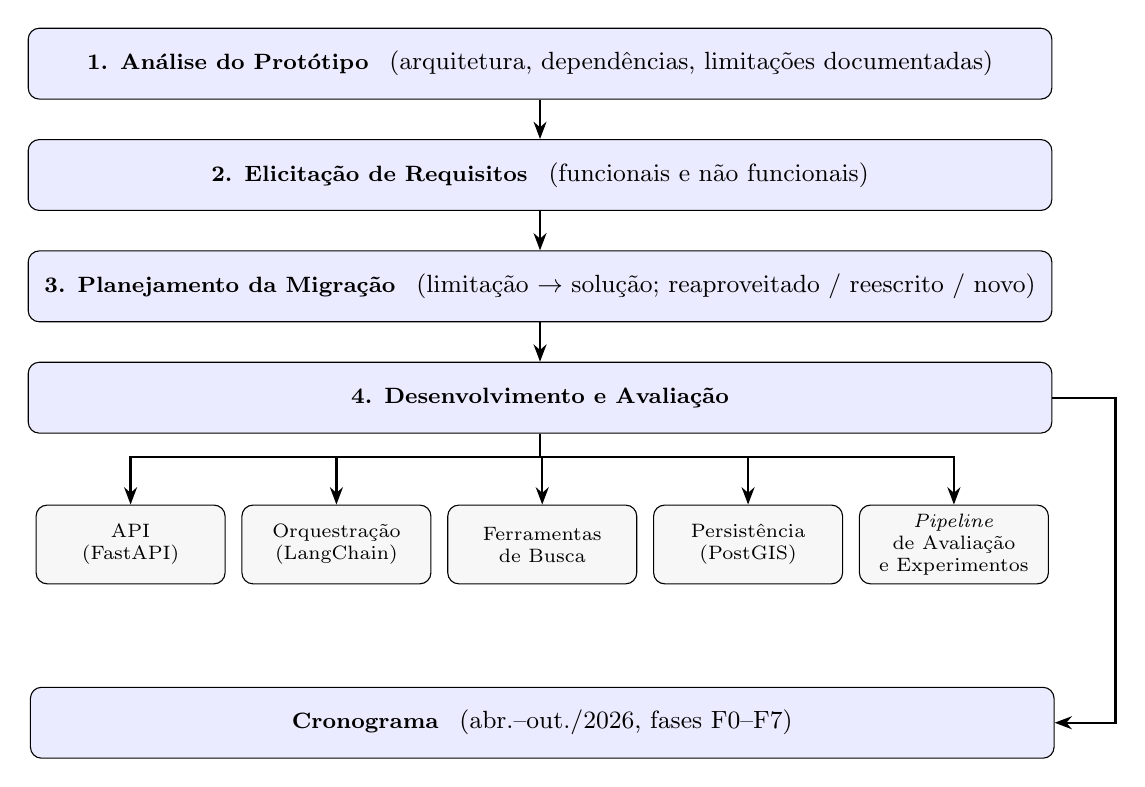
\begin{tikzpicture}[
  font=\footnotesize,
  node distance=0.5cm,
  eapstep/.style={rectangle, draw, rounded corners, minimum width=13cm, minimum height=0.9cm, align=center, fill=blue!8},
  sub/.style={rectangle, draw, rounded corners, minimum width=2.4cm, minimum height=1.0cm, align=center, fill=gray!6, font=\scriptsize, inner sep=2pt},
  arr/.style={-{Stealth[length=2.2mm]}, thick}
]
  \node[eapstep] (a) {\textbf{1. Análise do Protótipo} \;\;\small(arquitetura, dependências, limitações documentadas)};
  \node[eapstep, below=of a] (r) {\textbf{2. Elicitação de Requisitos} \;\;\small(funcionais e não funcionais)};
  \node[eapstep, below=of r] (p) {\textbf{3. Planejamento da Migração} \;\;\small(limitação $\to$ solução; reaproveitado / reescrito / novo)};
  \node[eapstep, below=of p] (d) {\textbf{4. Desenvolvimento e Avaliação}};
  \node[sub, below=0.9cm of d, xshift=-5.2cm] (s1) {API\\(FastAPI)};
  \node[sub, right=0.2cm of s1] (s2) {Orquestração\\(LangChain)};
  \node[sub, right=0.2cm of s2] (s3) {Ferramentas\\de Busca};
  \node[sub, right=0.2cm of s3] (s4) {Persistência\\(PostGIS)};
  \node[sub, right=0.2cm of s4] (s5) {\textit{Pipeline}\\de Avaliação\\e Experimentos};
  \node[eapstep, below=1.3cm of s3] (c) {\textbf{Cronograma} \;\;\small(abr.--out./2026, fases F0--F7)};
  \draw[arr] (a) to (r);
  \draw[arr] (r) to (p);
  \draw[arr] (p) to (d);
  \draw[arr] (d.south) to ++(0,-0.30) -| (s1.north);
  \draw[arr] (d.south) to ++(0,-0.30) -| (s2.north);
  \draw[arr] (d.south) to ++(0,-0.30) -| (s3.north);
  \draw[arr] (d.south) to ++(0,-0.30) -| (s4.north);
  \draw[arr] (d.south) to ++(0,-0.30) -| (s5.north);
  \draw[arr] (d.east) to ++(0.8,0) |- (c.east);
\end{tikzpicture}
\caption{Estrutura Analítica do Projeto (EAP)}
\label{fig:eap}
\fonte{Elaborado pelos autores.}
\end{figure}

% ============================================================
\section{Análise do Protótipo do 1º CGEO}
\label{sec:prototipo}
% ============================================================

\subsection{Arquitetura e Contribuições}

A Divisão de Levantamento ``Gen Augusto Tasso Fragoso'', do 1º CGEO, desenvolveu o protótipo como prova de conceito do uso de LLMs locais na busca sobre o catálogo sob sua guarda \cite{cgeo2025prototipo}. O código é público, e os 22 casos de teste do protótipo formam a camada P do \textit{dataset} de avaliação (Seção~\ref{sec:camadas}). A Figura~\ref{fig:arquitetura_prototipo} mostra as quatro camadas.

\begin{figure}[h]
\centering
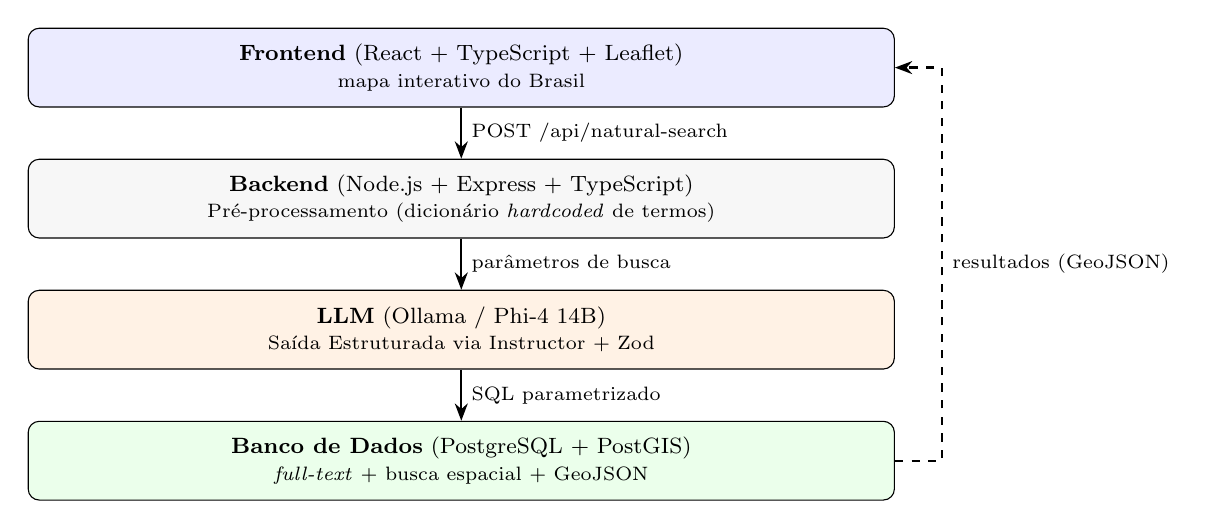
\begin{tikzpicture}[
  font=\footnotesize,
  node distance=0.65cm,
  layer/.style={rectangle, draw, rounded corners, minimum width=11cm, minimum height=1.0cm, align=center, fill=gray!6},
  arr/.style={-{Stealth[length=2.2mm]}, thick}
]
  \node[layer, fill=blue!8] (l1) {\textbf{Frontend} (React + TypeScript + Leaflet) \\ \scriptsize mapa interativo do Brasil};
  \node[layer, below=of l1] (l2) {\textbf{Backend} (Node.js + Express + TypeScript) \\ \scriptsize Pré-processamento (dicionário \textit{hardcoded} de termos)};
  \node[layer, below=of l2, fill=orange!10] (l3) {\textbf{LLM} (Ollama / Phi-4 14B) \\ \scriptsize Saída Estruturada via Instructor + Zod};
  \node[layer, below=of l3, fill=green!8] (l4) {\textbf{Banco de Dados} (PostgreSQL + PostGIS) \\ \scriptsize \textit{full-text} + busca espacial + GeoJSON};
  \draw[arr] (l1) to node[right, font=\scriptsize] {POST /api/natural-search} (l2);
  \draw[arr] (l2) to node[right, font=\scriptsize] {parâmetros de busca} (l3);
  \draw[arr] (l3) to node[right, font=\scriptsize] {SQL parametrizado} (l4);
  \draw[arr, dashed] (l4.east) to ++(0.6,0) |- node[right, font=\scriptsize, pos=0.25] {resultados (GeoJSON)} (l1.east);
\end{tikzpicture}
\caption{Arquitetura do protótipo de busca do 1º CGEO}
\label{fig:arquitetura_prototipo}
\fonte{Adaptado de \citeauthoronline{cgeo2025prototipo} (\citeyear{cgeo2025prototipo}).}
\end{figure}

O \textit{frontend}, em React com Leaflet, mostra os resultados num mapa do Brasil. O \textit{backend}, em Node.js com Express, recebe a consulta pela rota \texttt{POST /api/natural-search}. Antes do LLM, um pré-processador normaliza variações de grafia com um dicionário fixo no código (``25k'' $\rightarrow$ ``1:25.000''). O núcleo é o Phi-4 14B \cite{abdin2024phi4}, executado via Ollama, com Saída Estruturada pela biblioteca Instructor e \textit{schema} em Zod. O \textit{schema} pede um campo \texttt{reasoning}, em que o modelo justifica a extração, e os doze campos de busca (\texttt{keyword}, \texttt{scale}, \texttt{productType}, \texttt{state}, \texttt{city}, \texttt{supplyArea}, \texttt{project}, \texttt{publicationPeriod}, \texttt{creationPeriod}, \texttt{sortField}, \texttt{sortDirection} e \texttt{limit}). O \textit{prompt} traz exemplos resolvidos (\textit{few-shot prompting}). Se o LLM falhar mesmo após três novas tentativas, um \textit{fallback} por expressões regulares tenta extrair do texto parte dos campos (escala, tipo de produto, área de suprimento, projeto, ordenação, limite e períodos). O PostgreSQL/PostGIS combina busca textual com operações espaciais e devolve GeoJSON. O repositório traz o esquema do banco (\texttt{init.sql}, quatro tabelas), mas não os dados do acervo.

O protótipo demonstrou que (i) LLMs locais são tecnicamente viáveis no domínio cartográfico, (ii) o Phi-4 14B extrai parâmetros de busca relevantes de consultas em português, (iii) \textit{few-shot prompting} com Saída Estruturada produz resultados utilizáveis, o que este trabalho mediu na Seção~\ref{sec:abordagens}, e (iv) a integração do LLM com o PostgreSQL/PostGIS para busca espacial funciona em ambiente controlado.

\subsection{Limitações}
\label{sec:limitacoes}

O cliente apontou seis limitações do protótipo, que definem as frentes de aprimoramento:
\begin{enumerate}
  \item \textbf{\textit{Backend} em Node.js.} As bibliotecas de integração com LLMs (LangChain, LlamaIndex, Instructor) têm versões mais completas em Python.
  \item \textbf{Apenas Saída Estruturada.} O modelo devolve sempre a estrutura predefinida e não pode encadear ferramentas nem reagir ao resultado de operações anteriores.
  \item \textbf{Modelo único e defasado.} Com um só modelo, não há como comparar alternativas e escolher a mais adequada, num ecossistema que muda depressa.
  \item \textbf{Dicionário fixo no código.} O pré-processador aplica 159 pares de substituição antes de o texto chegar ao LLM. Variações não previstas no desenvolvimento (``dois cgeo'', ``25 mil'') falham em silêncio. A manutenção é manual, a partir dos erros vistos no \textit{log}. Um termo do dicionário em contexto ambíguo pode ainda deturpar uma consulta legítima.
  \item \textbf{\textit{Fallback} por expressões regulares.} Sua presença indica falhas do LLM que não foram documentadas de forma sistemática, o que dificulta a análise de causa.
  \item \textbf{Ausência de métricas de avaliação.} Os 22 casos de teste são pontuados por pesos atribuídos \textit{ad hoc} aos campos esperados, sem penalizar campos preenchidos indevidamente, e não há protocolo para comparar modelos, \textit{prompts} ou configurações.
\end{enumerate}

% ============================================================
\section{Requisitos}
\label{sec:requisitos}
\label{sec:requisitos-resumo}
% ============================================================

Os requisitos vieram da análise do protótipo e das conversas com o cliente. O Quadro~\ref{quadro:requisitos-resumo} traz cada um, a seção que o atende e como foi verificado. A latência (RNF2) depende do \textit{hardware} e da carga do ambiente de implantação, que estão fora do escopo. Por isso ela é reportada por ambiente (Seção~\ref{sec:ambiente}), sem limiar fixado \textit{a priori}.

\begin{quadro}[htbp!]
\centering
\caption{Requisitos da solução, onde são atendidos e como foram verificados}
\label{quadro:requisitos-resumo}
\footnotesize
\begin{tabular}{|c|>{\raggedright\arraybackslash}p{4.7cm}|>{\raggedright\arraybackslash}p{2.6cm}|>{\raggedright\arraybackslash}p{5.2cm}|}
\hline
\textbf{Requisito} & \textbf{Descrição} & \textbf{Atendido em} & \textbf{Verificação} \\
\hline
RF1 & Receber consulta em linguagem natural por rota REST & Seção~\ref{sec:api} & Demonstrado na API sobre os dados sintéticos; testes automatizados da API \\
\hline
RF2 & Traduzir a consulta nos doze parâmetros do \textit{schema} & Seção~\ref{sec:orquestracao} & Avaliado no Capítulo~\ref{cap:resultados} \\
\hline
RF3 & Executar a busca no PostgreSQL/PostGIS & Seção~\ref{sec:persistencia} & Demonstrado sobre os dados sintéticos; não avaliado \\
\hline
RF4 & Selecionar o modelo por requisição (só em desenvolvimento) & Seção~\ref{sec:api} & Implementado e coberto por teste da API; fora das métricas \\
\hline
RF5 & Registrar, por consulta, os parâmetros, as chamadas, os tempos e os erros, para o cálculo das métricas & Seção~\ref{sec:pipeline-avaliacao} & Registros e manifestos de todas as rodadas \\
\hline
RNF1 & Execução totalmente local & Seções~\ref{sec:orquestracao} e~\ref{sec:selecao-modelos} & Modelos locais; nuvem só como referência \\
\hline
RNF2 & Latência compatível com uso interativo & Seção~\ref{sec:ambiente} & Medida por ambiente, sem limiar fixado \\
\hline
RNF3 & Conformidade com a ET-PCDG e o Perfil MGB na estrutura dos metadados & Seção~\ref{sec:persistencia} & Esquema do protótipo reaproveitado; conformidade não verificada à parte \\
\hline
RNF4 & Reprodutibilidade dos experimentos & Seção~\ref{sec:reprodutibilidade} & Manifestos, \textit{hashes} e repontuação \\
\hline
RNF5 & Manutenibilidade & Seção~\ref{sec:harness} & Testes automatizados e integração contínua \\
\hline
RNF6 & Substituição do modelo por configuração & Seção~\ref{sec:harness} & Modelo e abordagem escolhidos por configuração \\
\hline
\end{tabular}%
\fonte{Elaborado pelos autores.}
\end{quadro}

% ============================================================
\section{Planejamento da Migração}
% ============================================================

A estratégia foi a \textbf{substituição dirigida}. Os componentes responsáveis pelas limitações da Seção~\ref{sec:limitacoes} foram substituídos, e o esquema do banco, os parâmetros de busca e a lógica das consultas espaciais foram aproveitados. O Quadro~\ref{quadro:mapa-limitacoes} liga cada limitação à solução adotada, e o Quadro~\ref{quadro:componentes} classifica cada componente do sistema final.

\begin{quadro}[h]
\centering
\caption{Mapeamento entre limitações do protótipo e soluções adotadas}
\label{quadro:mapa-limitacoes}
\small
\begin{tabular}{|c|>{\raggedright\arraybackslash}p{4.2cm}|>{\raggedright\arraybackslash}p{4.2cm}|>{\raggedright\arraybackslash}p{3.2cm}|}
\hline
\textbf{\#} & \textbf{Limitação} & \textbf{Solução adotada} & \textbf{Componente afetado} \\
\hline
1 & \textit{Backend} em Node.js & Reimplementação em Python com FastAPI & Nova API REST \\
\hline
2 & Apenas Saída Estruturada & \textit{Tool Calling} nativo via LangChain & Serviço de LLM \\
\hline
3 & Modelo único (Phi-4 14B) & Avaliação comparativa de quatro modelos atuais (Qwen 3 4B, Gemma 4 E2B, Gemma 4 E4B, Mistral Nemo 12B) & Configuração e testes \\
\hline
4 & Pré-processamento manual & Normalização delegada ao LLM, orientada pelas descrições do \textit{schema} da ferramenta & Remoção do pré-processador \\
\hline
5 & \textit{Fallback} via regex & Falhas registradas como métrica, sem \textit{fallback} oculto & Serviço de LLM \\
\hline
6 & Ausência de métricas & \textit{Dataset} auditado com gabarito + \textit{pipeline} de avaliação automatizado & Novo módulo de avaliação \\
\hline
\end{tabular}%
\fonte{Elaborado pelos autores.}
\nota{Soluções da v1. A v3 acrescenta, nas linhas 4 e 5, ferramentas auxiliares e o retorno de um validador (Seção~\ref{sec:orquestracao}).}
\end{quadro}

\begin{quadro}[h]
\centering
\caption{Classificação dos componentes do sistema final em relação ao protótipo}
\label{quadro:componentes}
\small
\begin{tabular}{|>{\raggedright\arraybackslash}p{4cm}|c|>{\raggedright\arraybackslash}p{6.5cm}|}
\hline
\textbf{Componente} & \textbf{Categoria} & \textbf{Observação} \\
\hline
Esquema do banco PostgreSQL/PostGIS & Reaproveitado & Mesmo esquema do protótipo (\texttt{init.sql}, quatro tabelas), sem alterações \\
\hline
Conjunto de parâmetros de busca & Reaproveitado & Os mesmos doze campos, compatíveis com a lógica das consultas SQL; enumerados recortados (9 tipos de produto e 9 projetos, contra 30 e 15 no protótipo) e grafados conforme a ET-PCDG \\
\hline
Lógica das consultas SQL & Reaproveitado & Portada de \texttt{search.ts}; direção de ordenação restrita a \texttt{ASC} ou \texttt{DESC}; aceita períodos com um só limite; sem o filtro por retângulo do mapa e a paginação, próprios do \textit{frontend} \\
\hline
\textit{Frontend} React/Leaflet & Fora do escopo & Não é parte deste trabalho \\
\hline
API REST & Reescrito & Node.js/Express $\to$ Python/FastAPI \\
\hline
Serviço de LLM & Reescrito & Saída Estruturada (Instructor/Zod) $\to$ \textit{Tool Calling} (LangChain) \\
\hline
Camada de acesso ao banco & Reescrito & \texttt{pg-promise} $\to$ \texttt{psycopg} \\
\hline
Pré-processamento de termos & Eliminado & Função transferida ao LLM \\
\hline
\textit{Fallback} com regex & Eliminado & Falhas viram métricas \\
\hline
Dados sintéticos do banco & Novo & Apenas para a demonstração ponta a ponta (Seção~\ref{sec:persistencia}) \\
\hline
\textit{Dataset} de avaliação & Novo & 310 consultas com gabarito auditado (Cap.~\ref{cap:metodologia} e Ap.~\ref{apendice:dataset}) \\
\hline
\textit{Pipeline} de avaliação & Novo & Execução, pontuação, conferência e relatórios (Seção~\ref{sec:pipeline-avaliacao}) \\
\hline
Ferramentas auxiliares e validador (v3) & Novo & No pacote, no avaliador e na API, como abordagem padrão (Seção~\ref{sec:v3}) \\
\hline
Registro de abordagens, testes e integração contínua & Novo & Registro único das configurações avaliadas, testes de regressão e guia de extensão (Seção~\ref{sec:harness}) \\
\hline
\end{tabular}%
\fonte{Elaborado pelos autores.}
\end{quadro}

% ============================================================
\section{Arquitetura da Solução v1}
\label{sec:desenvolvimento}
% ============================================================

A Figura~\ref{fig:arquitetura_proposta} mostra as camadas da solução. A v2 e a v3 mudam só a camada de tradução (Seções~\ref{sec:v2} e~\ref{sec:v3}). O padrão da API é hoje o \textit{Tool Calling} v3 com o Gemma 4 E4B (Seção~\ref{sec:harness}).

\begin{figure}[h]
\centering
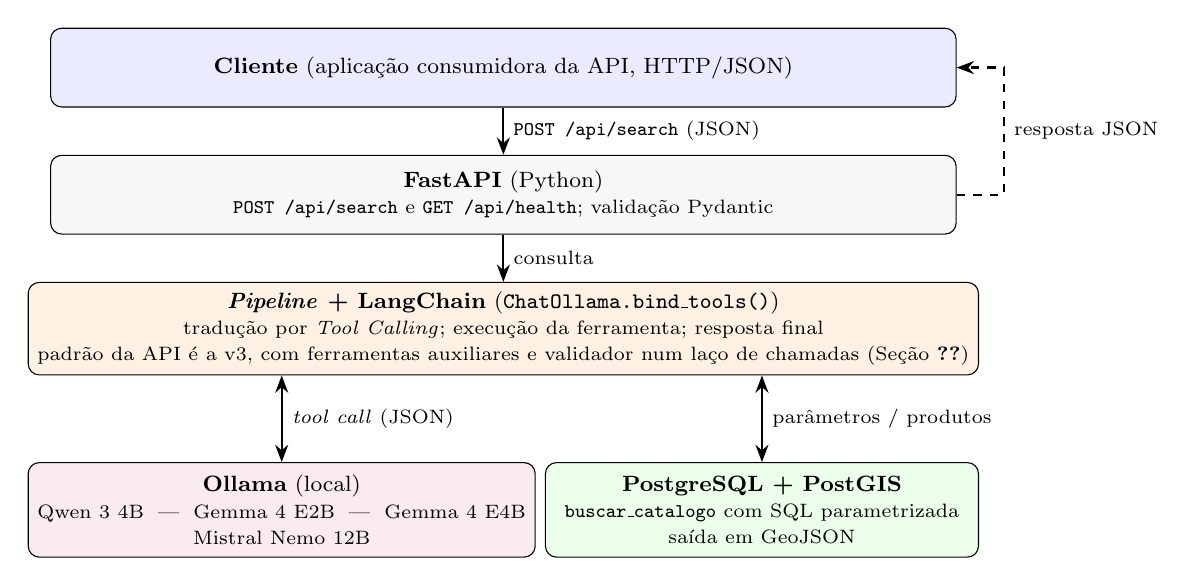
\begin{tikzpicture}[
  font=\footnotesize,
  node distance=0.6cm,
  layer/.style={rectangle, draw, rounded corners, minimum width=11.5cm, minimum height=1.0cm, align=center, fill=gray!6},
  half/.style={rectangle, draw, rounded corners, minimum width=5.5cm, minimum height=1.2cm, align=center, fill=gray!6},
  arr/.style={-{Stealth[length=2.2mm]}, thick},
  darr/.style={{Stealth[length=2.2mm]}-{Stealth[length=2.2mm]}, thick}
]
  \node[layer, fill=blue!8] (l1) {\textbf{Cliente} (aplicação consumidora da API, HTTP/JSON)};
  \node[layer, below=of l1] (l2) {\textbf{FastAPI} (Python) \\ \scriptsize \texttt{POST /api/search} e \texttt{GET /api/health}; validação Pydantic};
  \node[layer, below=of l2, fill=orange!10] (l3) {\textbf{\textit{Pipeline} + LangChain} (\texttt{ChatOllama.bind\_tools()}) \\ \scriptsize tradução por \textit{Tool Calling}; execução da ferramenta; resposta final \\ \scriptsize padrão da API é a v3, com ferramentas auxiliares e validador num laço de chamadas (Seção~\ref{sec:v3})};
  \node[half, below=1.1cm of l3.south west, anchor=north west, fill=purple!8] (l4) {\textbf{Ollama} (local) \\ \scriptsize Qwen 3 4B \;|\; Gemma 4 E2B \;|\; Gemma 4 E4B \\ \scriptsize Mistral Nemo 12B};
  \node[half, below=1.1cm of l3.south east, anchor=north east, fill=green!8] (l5) {\textbf{PostgreSQL + PostGIS} \\ \scriptsize \texttt{buscar\_catalogo} com SQL parametrizada \\ \scriptsize saída em GeoJSON};
  \draw[arr] (l1) to node[right, font=\scriptsize] {\texttt{POST /api/search} (JSON)} (l2);
  \draw[arr] (l2) to node[right, font=\scriptsize] {consulta} (l3);
  \draw[darr] (l4.north) to node[right, font=\scriptsize] {\textit{tool call} (JSON)} (l4.north |- l3.south);
  \draw[darr] (l5.north) to node[right, font=\scriptsize] {parâmetros / produtos} (l5.north |- l3.south);
  \draw[arr, dashed] (l2.east) to ++(0.6,0) |- node[right, font=\scriptsize, pos=0.25] {resposta JSON} (l1.east);
\end{tikzpicture}
\caption{Arquitetura da solução aprimorada de busca}
\label{fig:arquitetura_proposta}
\fonte{Elaborado pelos autores.}
\end{figure}

\subsection{API}
\label{sec:api}

A API REST usa o FastAPI~\cite{fastapi2018}, pela validação das requisições com Pydantic e pela documentação gerada automaticamente. A rota \texttt{POST /api/search} recebe a consulta e devolve os parâmetros extraídos, os produtos em GeoJSON, a resposta ao usuário, as latências e os erros. A rota \texttt{GET /api/health} informa a versão do Ollama, o estado do banco, o modelo e a abordagem no ar. O \textit{pipeline} de avaliação chama diretamente a camada de tradução, sem passar pela API, para que a latência medida seja a da chamada ao modelo.

\paragraph{Seleção de modelo.} A requisição pode escolher o modelo (RF4) só no ambiente de desenvolvimento. Em operação, o modelo é fixado por configuração, porque trocar de modelo entre requisições recarrega pesos na VRAM.

\paragraph{Tratamento de falhas.} Na v1 e na v2, cada falha do LLM é registrada como métrica, sem novas tentativas nem \textit{fallback} (limitação 5). As falhas se dividem em erros de infraestrutura (tempo esgotado, servidor ou modelo indisponível) e erros do modelo (argumentos fora do \textit{schema}, chamada a ferramenta inexistente). Um \textit{fallback} de produção fica como trabalho futuro (Seção~\ref{sec:trabalhos-futuros}).

\subsection{Orquestração e Ferramenta de Busca}
\label{sec:orquestracao}

A orquestração usa o \texttt{ChatOllama} do LangChain~\cite{langchain2022}, com a configuração da Seção~\ref{sec:config-modelos}. Na v1, a tradução é uma única chamada ao modelo, e o ciclo completo (executar a ferramenta e devolver o resultado ao modelo para a resposta final) é escrito no próprio módulo de \textit{pipeline}.

A ferramenta \texttt{buscar\_catalogo} tem os doze parâmetros de busca, cada um com tipo e, quando cabe, a lista fechada de valores válidos (o enumerado). Dez deles trazem na descrição instruções de normalização. O \textit{schema} fica num único módulo, que também serve para validar os argumentos do modelo e os enumerados do \textit{dataset}, e o seu \textit{hash} vai para o manifesto de cada rodada. Sem dicionário nem exemplos resolvidos no \textit{prompt}, o modelo normaliza os termos guiado só pelas descrições, que substituem as 159 entradas do dicionário do protótipo (limitação 4).

\begin{sloppypar}
A v1 expõe só \texttt{buscar\_catalogo}, e a v2 acrescenta \texttt{recusar\_consulta} (Seção~\ref{sec:v2}). A v3 (Seção~\ref{sec:v3}) acrescenta \texttt{identificar\_\allowbreak nome}, \texttt{normalizar\_\allowbreak codigo}, \texttt{normalizar\_\allowbreak escala}, \texttt{resolver\_\allowbreak periodo} e \texttt{pedir\_\allowbreak esclarecimento}. A v3 devolve parte da normalização ao código, em ferramentas que o modelo consulta quando precisa e num validador que confere a saída, e a consulta chega ao modelo sem reescrita prévia.
\end{sloppypar}

\subsection{Persistência}
\label{sec:persistencia}

O banco usa, sem alterações, o esquema do protótipo, em PostgreSQL com PostGIS~\cite{postgis2001}. Como o protótipo não traz os dados do acervo, a demonstração ponta a ponta usa dados sintéticos, gerados por \textit{script} com semente fixa (27 unidades da federação representadas por retângulos numa grade, 14 municípios, cinco áreas de suprimento e 117 produtos). \textbf{Nenhuma métrica deste trabalho depende do banco}, porque a avaliação incide sobre os parâmetros extraídos pelo modelo. O Docker Compose sobe o PostgreSQL 16 com PostGIS 3.4.

A lógica portada do \texttt{search.ts} combina busca textual, códigos MI e INOM, filtros, períodos, interseções espaciais, ordenação e limite, com os ajustes do Quadro~\ref{quadro:componentes}. As consultas são parametrizadas, e o modelo nunca escreve SQL.

Os enumerados do novo \textit{schema} grafam alguns valores de modo diferente do protótipo (acentos, travessões e nomes). Os dados sintéticos seguem a grafia nova, e ligar a API ao banco do acervo exige conferir a grafia guardada nele. A resolução dos campos geográficos em geometrias fica fora do escopo (Seção~\ref{sec:exclusoes-avaliacao}).

\subsection{Consultas sem Resposta no Acervo}
\label{sec:sem-resposta}

O sistema distingue três desfechos, e em nenhum deles inventa um produto:
\begin{enumerate}
  \item \textbf{Consulta fora do domínio do catálogo} (``cartas de Marte''). Não há busca. Na v1, o modelo não chama a ferramenta e responde em uma frase por que o pedido está fora do escopo. No \textit{Tool Calling} v2 e v3, ele chama \texttt{recusar\_consulta}, cujo argumento \texttt{motivo} é a frase dirigida ao usuário (na Saída Estruturada v2 e v3, a recusa é o campo \texttt{fora\_do\_escopo}). Na v3, a primeira recusa de uma consulta que cita um critério do catálogo volta ao modelo para confirmação (Seção~\ref{sec:v3}). A categoria F do \textit{dataset} mede esse comportamento.
  \item \textbf{Busca com produtos.} A lista vem sempre do banco, e o modelo só a resume.
  \item \textbf{Busca legítima sem produto.} A API devolve a lista vazia e uma mensagem fixa com os critérios usados, que sugere retirar ou ampliar algum deles, sem nova chamada ao modelo.
\end{enumerate}

Nos pedidos com valores que a ferramenta não representa (``escala 1:10.000.000'', ``cartas do estado 42''), o texto não determina o comportamento correto. O \textit{dataset} os trata como casos observacionais, fora das métricas principais (Seção~\ref{sec:observacionais}).

% ============================================================
\section{\textit{Pipeline} de Avaliação}
\label{sec:pipeline-avaliacao}
% ============================================================

O \textit{pipeline} de avaliação produz os números do Capítulo~\ref{cap:resultados}. Ele gera, da mesma fonte, o arquivo de consultas avaliado e as listagens do Apêndice~\ref{apendice:dataset}, validados contra o \textit{schema}, e roda as checagens automáticas da auditoria do gabarito (Seção~\ref{sec:auditoria}). Executa as consultas em ordem fixa, de forma sequencial e retomável, guarda a resposta, os tempos e os erros de cada consulta e repetição e grava um manifesto de reprodutibilidade por rodada (RNF4). A pontuação é sempre recalculada contra o gabarito vigente, e uma correção do gabarito não exige nova execução dos modelos. Antes da consolidação, ele confere os \textit{hashes} e a completude das rodadas. Depois gera as tabelas, as figuras e os testes estatísticos, inclusive os dos lotes e do teste A/B. A referência em nuvem roda no mesmo avaliador, pelo Groq (Apêndice~\ref{apx:specs-groq}). Os comandos estão no Apêndice~\ref{apx:comandos}.

\subsection{Registro de Abordagens e Implantação}
\label{sec:harness}

Um módulo único, o registro de abordagens, reúne as nove configurações avaliadas no estudo, da solução v1 às especificações v2 e v3 e ao método do protótipo (Quadro~\ref{quadro:desenho}). Os módulos das versões avaliadas ficam congelados, e um teste de regressão confere que o código atual reproduz os \textit{hashes} de \textit{prompt} e de ferramenta de todas as rodadas válidas.

A API escolhe a abordagem e o modelo por configuração (RNF6). O padrão é o \textit{Tool Calling} v3 com o Gemma 4 E4B (Seção~\ref{sec:recomendacao}), e a v1 continua disponível. O \texttt{/api/health} mostra os \textit{hashes} de \textit{prompt} e de ferramenta e as rodadas feitas com a mesma configuração, o que permite verificar se o que está no ar foi o avaliado. Na API, o pedido de esclarecimento da v3 continua respondido pelo usuário simulado da avaliação (Seção~\ref{sec:v3}), e levá-lo ao usuário real exige conversa em vários turnos (Seção~\ref{sec:trabalhos-futuros}). O índice de folhas do BDGEx, de que as ferramentas da v3 dependem, não está no repositório. Sem ele, a API sobe em modo degradado, com aviso, e o teste de regressão pula os casos da v3 (Apêndice~\ref{apendice:codigo}).

Um \textit{Dockerfile} empacota a API. Os testes automatizados cobrem o \textit{schema}, as consultas SQL, as métricas e a API, sem depender do Ollama nem do banco (RNF5), e a integração contínua os roda a cada mudança (Apêndice~\ref{apx:comandos}). Um guia de extensão exige que cada versão nova seja testada num conjunto ainda não usado, e uma v4 precisaria de um terceiro lote. Os autores implementaram muitas partes do sistema, e o restante do código e dos testes foi escrito com apoio do Claude Code, com os modelos Claude Opus 4.6 e Claude Opus 5.5, a partir da especificação deles (Tabela~\ref{tab:uso-ia}).

% ============================================================
\section{Cronograma}
\label{sec:cronograma}
% ============================================================

O projeto foi executado entre abril e outubro de 2026, em oito fases (Quadro~\ref{quadro:cronograma}). As fases F0, F1 e F5 correspondem aos pacotes de construção da EAP, e as fases F2, F3, F4 e F6 à avaliação, detalhada no Capítulo~\ref{cap:metodologia}. A F6 aparece dividida pelas datas do histórico do repositório.

\begin{quadro}[h]
\centering
\caption{Cronograma de execução do projeto}
\label{quadro:cronograma}
\small
\begin{tabular}{|c|p{6.6cm}|c|p{3.4cm}|}
\hline
\textbf{Fase} & \textbf{Atividade} & \textbf{Período} & \textbf{Marco} \\
\hline
F0 & Análise do protótipo: código-fonte, dependências, esquema do banco e limitações documentadas & abr/2026 & Limitações mapeadas \\
\hline
F1 & Elicitação de requisitos e planejamento da migração (limitação $\to$ solução; componentes reaproveitados, reescritos e novos) & mai/2026 & Requisitos e plano de migração \\
\hline
F2 & Referencial teórico; seleção dos modelos; definição das métricas e do protocolo de avaliação & mai--jun/2026 & Protocolo de avaliação \\
\hline
F3 & Construção do \textit{dataset} de avaliação: camadas P, N e G e respectivo gabarito (Apêndice~\ref{apendice:dataset}) & jun--jul/2026 & 310 consultas anotadas \\
\hline
F4 & Prova de conceito do \textit{Tool Calling} sobre consultas representativas, com modelo local e em nuvem & ago/2026 & Viabilidade do \textit{Tool Calling} demonstrada \\
\hline
F5 & Implementação: API, orquestração, ferramenta \texttt{buscar\_catalogo}, persistência e \textit{pipeline} de avaliação, com testes automatizados & set/2026 & Sistema ponta a ponta \\
\hline
F6a & Rodadas completas das 310 consultas, validação na estação de referência, referência em nuvem e auditoria do \textit{dataset} & 14--26/set/2026 & Resultados da v1 \\
\hline
F6b & Linhas de base com Saída Estruturada e método do protótipo; lote 1 e especificação v2 & 28/set/2026 & Comparação das abordagens \\
\hline
F6c & Rodadas do lote 1; v3 congelada; lote 2 e teste da v3 & 29/set/2026 & Teste da v3 \\
\hline
F6d & Extensão da v3 a outros modelos; registro de abordagens e API com a v3; teste A/B; latência na estação & 29--30/set/2026 & Recomendação \\
\hline
F7 & Redação dos resultados e da conclusão; preparação da defesa & set--out/2026 & Defesa (out/2026) \\
\hline
\end{tabular}%
\fonte{Elaborado pelos autores.}
\end{quadro}

% ----------------------------------------------------------
% Capítulo 5 — Resultados
% Tabelas, figuras e valores citados na prosa (\res{...}) são GERADOS por pfc-relatorio
% (pfc_busca/src/pfc_busca/evaluation/report.py) a partir de results/:
%   rodadas completas:  pfc-relatorio --modelos qwen3:4b-instruct-2507-q4_K_M,gemma4:e4b-it-qat,gemma4:e2b-it-qat,mistral-nemo:12b --comparar-com results/estacao --paper ../paper_revisado
%   estação:            pfc-relatorio --resultados results/estacao --modelos qwen3:4b-instruct-2507-q4_K_M,gemma4:e2b-it-qat --sufixo _estacao --titulo " --- estação de referência (camadas P e N)" --paper ../paper_revisado
%   nuvem:              pfc-relatorio --modelos <modelos do Groq com rodada completa> --sufixo _groq --titulo " --- referência em nuvem (Groq)" --paper ../paper_revisado
%   nuvem, mesmas consultas das rodadas completas:
%                       pfc-relatorio --modelos <idem> --sufixo _groqcomum --titulo " --- referência em nuvem, consultas das rodadas completas" --mesmas-consultas-de results --modelos-referencia <modelos locais> --saida results/consolidado_groqcomum --paper ../paper_revisado
%   reexecução na estação: ver o comentário da seção "Validação na Estação de Referência".
% Nenhum número deste capítulo é digitado à mão. A prosa interpretativa foi escrita sobre os valores
% gerados e deve ser relida sempre que as rodadas forem refeitas.
% ----------------------------------------------------------
\chapter{Resultados}
\label{cap:resultados}

% Guardas: o capítulo compila mesmo antes de os artefatos existirem.
\newcommand{\tabelagerada}[2]{\IfFileExists{tabelas/#1.tex}{\input{tabelas/#1}}{\par\noindent[DRAFT --- tabela \texttt{\detokenize{#1}} gerada por \texttt{pfc-relatorio}; #2]\par}}
\newcommand{\figuragerada}[3]{\IfFileExists{figuras/#1.pdf}{%
\begin{figure}[htbp!]\centering\includegraphics[width=0.92\textwidth]{figuras/#1.pdf}\caption{#2}\label{fig:#1}\fonte{Elaborado pelo autor.}\end{figure}}{\par\noindent[DRAFT --- figura \texttt{\detokenize{#1}}; #3]\par}}

Este capítulo apresenta os resultados da execução do protocolo descrito no Capítulo~\ref{cap:metodologia} sobre o \textit{dataset} do Apêndice~\ref{apendice:dataset}. Todos os valores são produzidos pelo \textit{pipeline} de avaliação (Seção~\ref{sec:pipeline-avaliacao}) a partir dos registros de execução, com a pontuação recalculada contra o gabarito vigente; cada rodada carrega um manifesto com a \textit{tag} e o \textit{digest} do modelo, as versões de \textit{software}, o \textit{hardware}, a data de referência e os \textit{hashes} do \textit{dataset} e da definição da ferramenta.

% ---
\section{Configuração Experimental}
\label{sec:config-experimental}
% ---

Os resultados vêm de três conjuntos de rodadas, descritos na Seção~\ref{sec:ambiente}: as \textbf{rodadas completas} dos quatro modelos locais, com três repetições, executadas com Ollama numa GPU de nuvem NVIDIA T4; a \textbf{validação na estação de referência}, com as 62 consultas das camadas P e N; e a \textbf{referência em nuvem}, com \res{groq}{geral}{nmodelos} modelos de maior porte servidos pelo Groq, com uma repetição. As Tabelas~\ref{tab:ambiente}, \ref{tab:ambiente_estacao} e~\ref{tab:ambiente_groq} transcrevem dos manifestos o ambiente de cada rodada. \res{principal}{geral}{frasecobertura}

\tabelagerada{tab_ambiente}{ambiente das rodadas completas}

Cada modelo foi avaliado com temperatura zero, limite de 1024 \textit{tokens} de saída, sem contexto de conversações anteriores (\textit{zero-shot}), sem exemplos no \textit{prompt} e sem dicionário de normalização, com o mesmo \textit{prompt} de sistema e a mesma definição da ferramenta \texttt{buscar\_catalogo}; o modo de raciocínio foi desativado nos modelos locais que o oferecem (Seção~\ref{sec:config-modelos}). As \textit{tags} exatas são \res{principal}{geral}{tags}. Nas rodadas completas, as métricas principais cobrem \res{principal}{geral}{nprincipais} consultas, pontuadas em cada uma das três repetições --- \res{principal}{qwen}{execucoes} execuções por modelo ---, incluindo as da categoria F, em que a resposta correta é não chamar a ferramenta; as consultas observacionais são reportadas à parte (Seção~\ref{sec:observacionais}). Nenhuma execução das rodadas completas terminou em erro de infraestrutura.

% ---
\section{Comparativo Geral entre Modelos}
\label{sec:comparativo}
% ---

A Tabela~\ref{tab:resultados_comparativo} sumariza as métricas principais por modelo, e a Tabela~\ref{tab:latencia} detalha a distribuição da latência da tradução.

\tabelagerada{tab_comparativo}{comparativo geral}

\tabelagerada{tab_latencia}{latência por modelo}

\paragraph{Qualidade.} Três dos quatro modelos ficaram num mesmo patamar de acurácia: \res{principal}{e4b}{acuracia} para o Gemma 4 E4B, \res{principal}{qwen}{acuracia} para o Qwen 3 4B e \res{principal}{e2b}{acuracia} para o Gemma 4 E2B, com intervalos de confiança que se sobrepõem amplamente. Pelo teste de McNemar (Seção~\ref{sec:estatistica}), nenhuma das diferenças entre esses três é estatisticamente significativa. O Mistral Nemo 12B, o maior dos quatro, ficou muito abaixo, com \res{principal}{mistral}{acuracia} (IC 95\%: \res{principal}{mistral}{ic}), e a diferença para cada um dos outros três é significativa. O tamanho do modelo, portanto, não explica o desempenho na tarefa: a Seção~\ref{sec:analise-erros} mostra que a queda do Mistral Nemo decorre quase inteiramente de um modo de falha no uso da ferramenta.

\paragraph{Precisão e \textit{recall}.} Os três modelos do patamar superior têm F1 ponderado semelhante (\res{principal}{qwen}{f1}, \res{principal}{e4b}{f1} e \res{principal}{e2b}{f1}), mas chegam a ele por caminhos diferentes. O Gemma 4 E4B tem a maior precisão (\res{principal}{e4b}{precisao}) e o menor \textit{recall} (\res{principal}{e4b}{recall}) dos três: quando chama a ferramenta, raramente preenche um campo errado, mas deixa de chamá-la com frequência. O Qwen 3 4B tem o maior \textit{recall} (\res{principal}{qwen}{recall}) e a menor precisão (\res{principal}{qwen}{precisao}), porque acrescenta com mais frequência campos que a consulta não pediu.

\paragraph{Latência.} Na T4, o Gemma 4 E2B foi o mais rápido, com mediana de \res{principal}{e2b}{latmeds}~s e percentil 95 de \res{principal}{e2b}{latpnoventaecinco}~s; o Gemma 4 E4B e o Qwen 3 4B tiveram medianas de \res{principal}{e4b}{latmeds}~s e \res{principal}{qwen}{latmeds}~s; e o Mistral Nemo 12B, \res{principal}{mistral}{latmeds}~s, cerca de \res{principal}{e2b-mistral}{razaolat} vezes a mediana do Gemma 4 E2B. A cauda do Gemma 4 E4B é mais longa que a do Qwen (percentil 95 de \res{principal}{e4b}{latpnoventaecinco}~s, contra \res{principal}{qwen}{latpnoventaecinco}~s), como mostra a Figura~\ref{fig:fig_latencia_boxplot}. Esses tempos valem para uma GPU com VRAM suficiente para cada modelo inteiro; na estação de referência, com 4~GB, a latência é maior e depende da parcela do modelo que cabe na GPU (Seção~\ref{sec:validacao-local}).

\figuragerada{fig_latencia_boxplot}{Distribuição da latência da tradução nas rodadas completas, em escala logarítmica, por modelo}{boxplot de latência}

\paragraph{Estabilidade entre repetições.} Numa mesma sessão da T4, as três repetições produziram exatamente a mesma resposta em \res{principal}{qwen}{estaveis} das \res{principal}{qwen}{nestaveis} consultas para o Qwen 3 4B, em \res{principal}{e2b}{estaveis} para o Gemma 4 E2B, em \res{principal}{mistral}{estaveis} para o Mistral Nemo 12B e em \res{principal}{e4b}{estaveis} para o Gemma 4 E4B. Com temperatura zero e o mesmo ambiente, a variação entre repetições foi, portanto, pequena; a Seção~\ref{sec:validacao-local} mostra que ela é maior entre sessões diferentes na estação de referência.

% ---
\section{Análise por Categoria de Consulta}
\label{sec:por-categoria}
% ---

A Tabela~\ref{tab:resultados_por_categoria} apresenta o F1 ponderado por categoria, e a Figura~\ref{fig:fig_acuracia_por_categoria}, a acurácia por consulta. A categoria F aparece só na figura: como o gabarito dessas consultas não tem campos, a acurácia nela é a taxa de recusa correta.

\tabelagerada{tab_por_categoria}{F1 por categoria}

\figuragerada{fig_acuracia_por_categoria}{Acurácia por consulta, por categoria e por modelo, nas rodadas completas}{acurácia por categoria}

\paragraph{O que é fácil.} As consultas simples, com um único parâmetro, tiveram as maiores acurácias entre as categorias com campos: \res{principal}{e4b}{accS} no Gemma 4 E4B e \res{principal}{qwen}{accS} no Qwen 3 4B e no Gemma 4 E2B. Os quatro modelos recusaram corretamente as consultas fora do domínio --- a acurácia na categoria F foi de \res{principal}{qwen}{accF}, \res{principal}{e4b}{accF}, \res{principal}{e2b}{accF} e \res{principal}{mistral}{accF} para Qwen 3 4B, Gemma 4 E4B, Gemma 4 E2B e Mistral Nemo 12B ---, o que confirma que o \textit{Tool Calling} permite ao modelo decidir não buscar, algo que a Saída Estruturada do protótipo não permitia.

\paragraph{O que é difícil para todos.} As categorias de tempo relativo e de ordenação foram as mais difíceis para os quatro modelos. No tempo relativo, a melhor acurácia foi a do Qwen 3 4B, \res{principal}{qwen}{accT}; na ordenação, nenhum modelo passou de \res{principal}{qwen}{accO}, e o Gemma 4 E2B não acertou nenhuma consulta dessa categoria. As consultas compostas, que exigem vários campos corretos ao mesmo tempo, ficaram em torno de \res{principal}{qwen}{accC} a \res{principal}{e4b}{accC} nos três melhores modelos. Essas quedas simultâneas indicam dificuldades da tarefa, e não de um modelo específico: resolver uma expressão temporal em datas ISO e decidir se, e por qual data, ordenar são as etapas em que a tradução mais depende de raciocínio além do reconhecimento de nomes.

\paragraph{Onde os modelos divergem.} Nas consultas com código MI ou INOM, o Qwen 3 4B foi o mais consistente (\res{principal}{qwen}{accM}, contra \res{principal}{e2b}{accM} do Gemma 4 E2B e \res{principal}{e4b}{accM} do Gemma 4 E4B). Nas consultas ambíguas e informais, o Gemma 4 E4B teve a maior acurácia (\res{principal}{e4b}{accA}).

% ---
\section{Análise por Campo do \textit{Schema}}
\label{sec:por-campo}
% ---

\tabelagerada{tab_por_campo}{F1 por campo}

\figuragerada{fig_f1_por_campo}{F1-\textit{score} por campo do \textit{schema} de busca, por modelo, nas rodadas completas}{F1 por campo}

Os campos de identificação --- \texttt{supplyArea}, \texttt{city}, \texttt{project} e \texttt{keyword} --- tiveram, em geral, os maiores F1 nos três melhores modelos: o Gemma 4 E2B acertou todas as ocorrências de \texttt{supplyArea} (F1 de \res{principal}{e2b}{f1supplyArea}), e o Qwen 3 4B teve o maior F1 em \texttt{keyword} (\res{principal}{qwen}{f1keyword}), coerente com seu desempenho nas consultas com código MI/INOM. São campos em que a tarefa se reduz a reconhecer e normalizar um nome, justamente o que o dicionário fixo do protótipo fazia; aqui, a normalização foi feita pelo próprio modelo, a partir das descrições da ferramenta.

Os campos de período e de ordenação concentraram as perdas. O F1 de \texttt{publicationPeriod} ficou entre \res{principal}{e4b}{f1publicationPeriod} (Gemma 4 E4B) e \res{principal}{e2b}{f1publicationPeriod} (Gemma 4 E2B), e os de \texttt{sortField} e \texttt{sortDirection} não passaram de \res{principal}{qwen}{f1sortField} em nenhum dos quatro modelos. O campo \texttt{creationPeriod} tem poucas ocorrências nas consultas pontuadas, o que torna seu F1 instável.

% ---
\section{Análise de Erros}
\label{sec:analise-erros}
% ---

A classificação dos erros (Seção~\ref{sec:metricas}) mostra um modo de falha dominante diferente em cada modelo. Os exemplos citados são da primeira repetição e estão, com os demais, no arquivo \texttt{results/consolidado/erros\_representativos.md} do repositório.

\paragraph{Mistral Nemo 12B: a chamada descrita em texto.} O Mistral Nemo 12B deixou de chamar a ferramenta em \res{principal}{mistral}{erronaochamou} das \res{principal}{mistral}{execucoes} execuções pontuadas. Em \res{principal}{mistral}{naochamounarrada} delas, a resposta cita a ferramenta \texttt{buscar\_catalogo} e descreve, em texto corrido, a chamada que faria. Para ``preciso da carta MI 2965-2-NE do segundo cgeo'', por exemplo, o modelo respondeu que chamaria a ferramenta com \texttt{keyword} ``2965-2-NE'' e \texttt{supplyArea} ``2° Centro de Geoinformação'', mas não emitiu a chamada estruturada. Em outras \res{principal}{mistral}{naochamouesclarecimento}, pediu mais informações ao usuário. Nesses casos, o modelo identifica a ferramenta e os parâmetros, mas não emite a chamada no canal de \textit{tool calls} da integração com o Ollama; como o protocolo não interpreta texto livre como chamada, cada um deles conta como falha.

\paragraph{Gemma 4 E4B e E2B: o pedido de esclarecimento.} Os dois modelos Gemma deixaram de chamar a ferramenta em \res{principal}{e4b}{erronaochamou} (E4B) e \res{principal}{e2b}{erronaochamou} (E2B) execuções, quase sempre pedindo ao usuário que especificasse melhor a busca --- \res{principal}{e4b}{naochamouesclarecimento} e \res{principal}{e2b}{naochamouesclarecimento} casos, respectivamente. Isso ocorreu sobretudo em consultas amplas, com um único critério: ``cartas topográficas'', ``produtos em escala 1:50.000'', ``modelos digitais de terreno''. O Gemma 4 E2B cometeu ainda um erro próprio, o campo acrescentado mais frequente nas suas respostas: copiar para \texttt{keyword} palavras comuns da consulta, como ``mdt'' em ``mdt do para em 25k'' ou ``mapeamento detalhado'' em ``mapeamento detalhado (25k ou 50k) de brasilia''.

\paragraph{Qwen 3 4B: a recusa indevida e os campos acrescentados.} O Qwen 3 4B chamou a ferramenta com mais regularidade, mas declarou fora do escopo \res{principal}{qwen}{naochamouescopo} execuções de consultas legítimas, como ``primeiro mapeamento feito em cuiaba'' e ``ultima atualizacao do para''. Seu erro mais frequente, porém, foi acrescentar campos não pedidos, sobretudo ordenação e limite (\texttt{sortField}, \texttt{sortDirection} e \texttt{limit} são os campos mais frequentes entre os seus falsos positivos): para ``todas as cartas em escala maior que 100k do rio grande do sul'', emitiu ordenação decrescente por data de publicação e limite de 100 resultados, e omitiu a escala.

\paragraph{Datas relativas.} Os erros em períodos seguem padrões comuns aos modelos: tratar ``esse ano'' como começando na data de referência, e não em 1º de janeiro; reduzir ``2 anos atrás'' a um único dia; e trocar o trimestre-calendário por três meses corridos, ou pelo trimestre errado, em ``trimestre passado'' e ``último trimestre do ano passado''. A Tabela~\ref{tab:resultados_por_campo} mostra o efeito desses erros no F1 dos campos de período.

Os tipos de erro têm, assim, remédios diferentes. A chamada descrita em texto do Mistral Nemo é uma limitação da integração do modelo com o canal de ferramentas. O pedido de esclarecimento dos modelos Gemma e a recusa indevida do Qwen são decisões de chamar ou não, sensíveis à redação do \textit{prompt}. Os erros de período e de ordenação são erros de raciocínio sobre a consulta. Nenhum deles decorre de valores fora do \textit{schema}: não houve, em nenhum modelo, argumento com campo inexistente ou tipo inválido.

\subsection{Casos observacionais}
\label{sec:observacionais}

As quatro consultas observacionais testam o comportamento diante de pedidos que a ferramenta não consegue representar. O Qwen 3 4B foi o único que chamou a ferramenta nas duas consultas com valor impossível, em \res{principal}{qwen}{obschamou} das \res{principal}{qwen}{obsn} execuções observacionais: para ``escala 1:10.000.000'', emitiu a escala 1:10.000, que existe no enumerado mas não corresponde ao pedido; para ``cartas do estado 42'', emitiu \texttt{state} ``Rio Grande do Sul'', um valor sem nenhum apoio no texto. Os demais modelos não chamaram a ferramenta nesses dois casos. Nas consultas de resposta discutível --- ``cartas topo no oceano atlântico'' e ``cartas do futuro (ano 2050)'' ---, os modelos em geral também não chamaram a ferramenta; o Gemma 4 E2B buscou cartas topográficas sem restrição de área na primeira delas.

% ---
\section{Validação na Estação de Referência}
\label{sec:validacao-local}
% ---

% Reexecução (tab_concordancia_reexecucao, numeros_reexecucao):
%   pfc-relatorio --resultados results/estacao --modelos qwen3:4b-instruct-2507-q4_K_M --comparar-com results/_descartados/estacao_14set_vram_disputada --nome-comparacao reexecucao --rotulos-comparacao "24/set,14/set" --legenda-comparacao "Qwen 3 4B executado duas vezes na estação de referência, com os mesmos pesos, prompt, ferramenta e data de referência (camadas P e N)" --so-comparacao --saida results/estacao/consolidado --paper ../paper_revisado
As 62 consultas das camadas P e N foram executadas na estação de referência pelos dois modelos de menor porte, Qwen 3 4B e Gemma 4 E2B, com uma repetição e a mesma data de referência das rodadas completas. As duas rodadas foram feitas em sequência, na mesma sessão. Antes de cada uma, o \textit{pipeline} descarregou do Ollama todos os modelos residentes, de modo que cada modelo foi carregado a frio, com a VRAM que a estação tinha livre (Tabela~\ref{tab:ambiente_estacao}). Com 4~GB de VRAM, nenhum dos dois coube inteiro na GPU: o Ollama alocou na VRAM \res{estacao}{qwen}{nagpu} do Qwen 3 4B carregado, contando pesos e contexto, e \res{estacao}{e2b}{nagpu} do Gemma 4 E2B; o restante executou na CPU.

\tabelagerada{tab_ambiente_estacao}{ambiente da validação na estação}

\tabelagerada{tab_comparativo_estacao}{comparativo na estação}

\tabelagerada{tab_latencia_estacao}{latência na estação}

\paragraph{Qualidade.} Nas \res{estacao}{qwen}{n} consultas pontuadas, os dois modelos tiveram acurácias estatisticamente indistinguíveis: \res{estacao}{qwen}{acuracia} para o Qwen 3 4B (IC 95\%: \res{estacao}{qwen}{ic}) e \res{estacao}{e2b}{acuracia} para o Gemma 4 E2B (IC 95\%: \res{estacao}{e2b}{ic}). Entre as consultas acertadas por apenas um deles, \res{estacao}{qwen-e2b}{soa} foram do Qwen e \res{estacao}{qwen-e2b}{sob} do Gemma, com \textit{p}-valor de \res{estacao}{qwen-e2b}{p} no teste de McNemar exato (Tabela~\ref{tab:mcnemar_estacao}).

\tabelagerada{tab_mcnemar_estacao}{McNemar na estação}

\paragraph{Latência.} A latência, ao contrário, separou nitidamente os dois modelos. O Qwen 3 4B teve mediana de \res{estacao}{qwen}{latmeds}~s e percentil 95 de \res{estacao}{qwen}{latpnoventaecinco}~s; o Gemma 4 E2B, \res{estacao}{e2b}{latmeds}~s e \res{estacao}{e2b}{latpnoventaecinco}~s, cerca de \res{estacao}{qwen-e2b}{razaolat} vezes mais rápido, apesar da menor parcela na GPU. Dois fatores são compatíveis com essa diferença: o Gemma 4 E2B computa com cerca de 2 bilhões de parâmetros efetivos (Seção~\ref{sec:selecao-modelos}), e suas respostas foram mais curtas, com mediana de \res{estacao}{e2b}{toksaida} \textit{tokens} de saída, contra \res{estacao}{qwen}{toksaida} do Qwen 3 4B. Em relação à T4, a latência mediana do Qwen 3 4B subiu de \res{principal}{qwen}{latmeds}~s para \res{estacao}{qwen}{latmeds}~s, e a do Gemma 4 E2B, de \res{principal}{e2b}{latmeds}~s para \res{estacao}{e2b}{latmeds}~s.

\figuragerada{fig_latencia_boxplot_estacao}{Distribuição da latência da tradução na estação de referência, em escala logarítmica}{boxplot de latência na estação}

\paragraph{Comportamento.} Na categoria F, a acurácia foi de \res{estacao}{qwen}{accF} para o Qwen 3 4B e de \res{estacao}{e2b}{accF} para o Gemma 4 E2B: os dois recusaram as consultas fora do domínio das camadas P e N. Os modos de falha foram os mesmos das rodadas completas: o Qwen declarou fora do escopo pedidos como ``atualizações deste mês'', e o Gemma pediu mais critérios em consultas como ``cartas topográficas'' e ``produtos publicados nos últimos 3 meses'', contrariando a instrução do \textit{prompt} de sistema de que um único parâmetro basta para chamar a ferramenta.

\figuragerada{fig_acuracia_por_categoria_estacao}{Acurácia por consulta, por categoria, na estação de referência}{acurácia por categoria na estação}

\paragraph{Comparação com as rodadas completas.} A Tabela~\ref{tab:concordancia-ambientes} compara, para os mesmos modelos e consultas, as respostas da estação com as da primeira repetição das rodadas completas. A resposta foi idêntica em \res{ambientes}{qwen}{identicas} das \res{ambientes}{qwen}{n} consultas para o Qwen 3 4B e em \res{ambientes}{e2b}{identicas} para o Gemma 4 E2B, e a pontuação coincidiu em \res{ambientes}{qwen}{mesmanota} e \res{ambientes}{e2b}{mesmanota}, respectivamente. A acurácia nessas consultas foi de \res{ambientes}{qwen}{acuraciaa} e \res{ambientes}{e2b}{acuraciaa} nas rodadas completas, e de \res{ambientes}{qwen}{acuraciab} e \res{ambientes}{e2b}{acuraciab} na estação. A qualidade da tradução, portanto, praticamente não mudou com o \textit{hardware}; a latência, sim.

\tabelagerada{tab_concordancia_ambientes}{concordância entre a estação e as rodadas completas}

\paragraph{Reexecução na mesma estação.} O Qwen 3 4B já havia executado as mesmas consultas na estação em 14 de setembro de 2026, com os mesmos pesos, \textit{prompt}, ferramenta, data de referência e versão do Ollama. A Tabela~\ref{tab:concordancia-reexecucao} compara as duas execuções: mesmo com temperatura zero, a resposta se repetiu em \res{reexecucao}{qwen}{identicas} das \res{reexecucao}{qwen}{n} consultas, e a pontuação, em \res{reexecucao}{qwen}{mesmanota}. A explicação mais provável são diferenças numéricas de ponto flutuante na inferência, que dependem da divisão do modelo entre GPU e CPU e da ordem das operações e bastam para mudar a escolha de um \textit{token} em respostas isoladas. A variação é maior entre sessões na estação, com parte do modelo na CPU, do que entre as repetições de uma mesma sessão na T4 (Seção~\ref{sec:comparativo}), e é por causa dela que as rodadas completas usam três repetições e que a acurácia é reportada com intervalo de confiança.

\tabelagerada{tab_concordancia_reexecucao}{reexecução do Qwen 3 4B na estação}

% ---
\section{Referência em Nuvem}
\label{sec:referencia-nuvem}
% ---

\res{groq}{geral}{nmodelosmaiusc} modelos de maior porte servidos pelo Groq executaram o mesmo protocolo, com uma repetição: \res{groq}{geral}{tags}. Eles não atendem ao requisito de execução local (RNF1) e servem como referência de quanto modelos maiores, sem restrição de \textit{hardware}, acertam nas mesmas consultas; a latência inclui a rede e não é comparável à dos modelos locais.

\tabelagerada{tab_ambiente_groq}{ambiente da referência em nuvem}

\tabelagerada{tab_comparativo_groq}{comparativo da referência em nuvem}

\tabelagerada{tab_por_categoria_groq}{F1 por categoria na referência em nuvem}

Sobre todas as \res{groq}{gptoss20}{n} consultas das métricas principais, o GPT-OSS 20B acertou \res{groq}{gptoss20}{acuracia} (IC 95\%: \res{groq}{gptoss20}{ic}) e o GPT-OSS 120B, \res{groq}{gptoss120}{acuracia} (IC 95\%: \res{groq}{gptoss120}{ic}). Restrita às mesmas \res{groqcomum}{gptoss20}{n} consultas pontuadas nas rodadas completas dos modelos locais, a acurácia foi de \res{groqcomum}{gptoss20}{acuracia} e \res{groqcomum}{gptoss120}{acuracia}, respectivamente, contra \res{principal}{e4b}{acuracia} do melhor modelo local. A distância é maior justamente nas categorias difíceis para os modelos locais: nas consultas compostas e de tempo relativo desse mesmo conjunto, o GPT-OSS 20B acertou \res{groqcomum}{gptoss20}{accC} e \res{groqcomum}{gptoss20}{accT}, contra no máximo \res{principal}{e4b}{accC} e \res{principal}{qwen}{accT} entre os modelos locais. A ordenação continuou sendo a categoria mais difícil também para eles: sobre todo o \textit{dataset}, o GPT-OSS 20B acertou \res{groq}{gptoss20}{accO} dessas consultas e o GPT-OSS 120B, \res{groq}{gptoss120}{accO}. Como nas rodadas locais, todas as consultas fora do domínio foram recusadas.

A referência mostra que a tarefa, com a mesma ferramenta, o mesmo \textit{prompt} e o mesmo gabarito, é resolvível com alta acurácia por modelos de maior porte. A distância para os modelos locais mede, assim, a limitação dos modelos que cabem em estações modestas, e não um defeito do protocolo ou do gabarito.

% ---
\section{Análise Estatística}
\label{sec:estatistica}
% ---

A Tabela~\ref{tab:mcnemar} traz o teste de McNemar exato entre cada par de modelos das rodadas completas, sobre as mesmas consultas e repetições. Entre os três modelos do patamar superior, nenhuma diferença é significativa: o \textit{p}-valor foi de \res{principal}{qwen-e4b}{p} entre Qwen 3 4B e Gemma 4 E4B, de \res{principal}{qwen-e2b}{p} entre Qwen 3 4B e Gemma 4 E2B e de \res{principal}{e4b-e2b}{p} entre os dois Gemma. Entre o Mistral Nemo 12B e cada um dos outros três, o \textit{p}-valor foi \res{principal}{qwen-mistral}{p}. Como as três repetições de cada consulta entram como pares, e elas são quase sempre idênticas numa mesma sessão, os testes tratam como independentes observações que não o são inteiramente; os \textit{p}-valores devem ser lidos como aproximação, o que não altera as conclusões, dada a distância entre os dois grupos de modelos e a proximidade dentro do grupo superior.

\tabelagerada{tab_mcnemar}{McNemar entre pares de modelos}

% ---
\section{Discussão}
\label{sec:discussao}
% ---

\paragraph{Qualidade e latência.} Os resultados não apontam um modelo dominante em qualidade entre Qwen 3 4B, Gemma 4 E4B e Gemma 4 E2B: as acurácias são estatisticamente indistinguíveis, e cada um tem pontos fortes próprios --- o Qwen nos códigos MI/INOM e no \textit{recall}, o Gemma 4 E4B na precisão e nas consultas informais, o Gemma 4 E2B nos campos de escala, tipo de produto e área de suprimento. A latência os separa com mais clareza: o Gemma 4 E2B foi o mais rápido tanto na T4 quanto na estação de referência, onde sua mediana ficou abaixo de um segundo.

\paragraph{O que o \textit{Tool Calling} entregou.} Em relação à Saída Estruturada do protótipo, três ganhos aparecem diretamente nos dados. O modelo passou a poder recusar: todas as consultas fora do domínio foram recusadas por todos os modelos. A normalização de siglas, grafias sem acento, apelidos de escala e nomes de projeto passou a ser feita pelo modelo, sem dicionário, com F1 elevado nos campos de identificação. E toda falha passou a ser registrada e classificada, o que permitiu identificar o modo de falha de cada modelo --- inclusive o do Mistral Nemo 12B, que um mecanismo de \textit{fallback} teria mascarado.

\paragraph{O que continua difícil.} Datas relativas, ordenação e consultas com muitos campos permanecem difíceis para todos os modelos locais, e a ordenação o é também para os modelos em nuvem. Parte da dificuldade é inerente à tarefa: nem sempre a consulta diz se a ordem é por publicação ou por criação, e o gabarito aceita as duas leituras, mas os modelos ainda assim acrescentam ou omitem campos. Outra parte é sensível ao \textit{prompt}: a recusa indevida e o pedido de esclarecimento em consultas amplas contrariam uma instrução explícita e são candidatos naturais a ajuste de \textit{prompt} ou a exemplos no \textit{prompt}, que este trabalho não usou por desenho.

\paragraph{\textit{Hardware}.} Com 4~GB de VRAM, nenhum modelo coube inteiro na GPU da estação, e a latência depende diretamente da parcela alocada. A qualidade, por outro lado, praticamente não mudou entre a estação e a T4. Para a DSG, isso significa que a escolha do modelo pode ser feita pela qualidade medida em qualquer ambiente, e que o \textit{hardware} de implantação define a latência: uma GPU com 6 a 8~GB de VRAM já comportaria inteiros o Qwen 3 4B e o Gemma 4 E2B.

\subsection{Recomendação de Modelo para Uso Operacional}

Para o uso operacional sobre o acervo da DSG, em estações com GPU modesta, recomenda-se o \textbf{Gemma 4 E2B}: sua acurácia é estatisticamente equivalente à dos melhores modelos avaliados, e ele teve a menor latência nos dois ambientes, inclusive na estação de referência de 4~GB. O \textbf{Qwen 3 4B} é a alternativa quando as consultas com códigos MI/INOM forem predominantes, categoria em que teve o melhor desempenho, ao custo de uma latência maior na estação. O Gemma 4 E4B, de qualidade equivalente, exige mais VRAM que os outros dois e não foi medido na estação de referência. O Mistral Nemo 12B não é recomendado na configuração avaliada, pela falha sistemática no uso do canal de ferramentas.

A recomendação tem três ressalvas. Ela vale para a configuração avaliada --- sem raciocínio, sem exemplos no \textit{prompt} e com as versões registradas nos manifestos ---, e o desempenho com raciocínio ativado não foi medido. A distância para os modelos em nuvem indica margem de melhoria considerável, que pode vir de novos modelos abertos: o \textit{pipeline} permite repetir a comparação com o mesmo critério. E os modos de falha identificados, sobretudo o pedido de esclarecimento em consultas amplas, devem ser observados no uso real antes da implantação em larga escala.

% ----------------------------------------------------------
% Capítulo 6 — Conclusão
% ----------------------------------------------------------
\chapter{Conclusão}
\label{cap:conclusao}

% ---
\section{Síntese do Trabalho}
% ---

Este Projeto Final de Curso aprimorou a camada de tradução linguística da solução de busca em linguagem natural sobre o acervo cartográfico da Diretoria de Serviço Geográfico (DSG), partindo do protótipo desenvolvido pelo 1º Centro de Geoinformação (1º CGEO). O protótipo demonstrou a viabilidade da abordagem, mas apresentava limitações documentadas pelo próprio cliente: \textit{backend} em Node.js, Saída Estruturada via Instructor e Zod, um único modelo (Phi-4 14B), dicionário de normalização fixo no código, \textit{fallback} por expressões regulares e ausência de um protocolo de avaliação.

A partir da análise crítica do protótipo, o trabalho entregou:

\begin{enumerate}
  \item um \textit{backend} em Python, com FastAPI e LangChain, que substitui o do protótipo e preserva o esquema do banco e o conjunto de parâmetros de busca;
  \item a substituição da Saída Estruturada por \textit{Tool Calling} nativo, em que o modelo decide se chama a ferramenta de busca e com quais argumentos, sem dicionário de normalização e sem exemplos resolvidos no \textit{prompt};
  \item um \textit{dataset} de avaliação com 310 consultas, construído em três camadas (protótipo, autores e geração programática), com gabarito definido por um manual de anotação escrito, leituras múltiplas explícitas para as consultas ambíguas e uma auditoria em três etapas --- checagens automáticas, anotação independente às cegas e adjudicação registrada --- que deixou todas as divergências com decisão justificada;
  \item um \textit{pipeline} de avaliação automatizado e reprodutível, que registra manifesto e traços de cada rodada, recalcula a pontuação contra o gabarito vigente e produz acurácia com intervalo de confiança, precisão, \textit{recall} e F1 por campo, latência e testes de significância entre modelos;
  \item a comparação de quatro modelos abertos executáveis localmente --- Qwen 3 4B, Gemma 4 E4B, Gemma 4 E2B e Mistral Nemo 12B ---, complementada por uma referência paralela com \res{groq}{geral}{nmodelos} modelos de maior porte servidos em nuvem;
  \item um lote de validação independente (lote 1), de \res{lotedados}{geral}{aceitas} consultas com gabarito fixado antes da redação e aceitas por anotação às cegas, sobre o qual as duas abordagens foram comparadas com a especificação da solução e com uma segunda especificação (v2), para separar o efeito da abordagem do efeito da especificação;
  \item a v3 do \textit{Tool Calling}, com ferramentas auxiliares determinísticas e validação com retorno, desenvolvida sobre as 310 consultas e os erros de uma amostra do lote 1 e testada, contra um controle de Saída Estruturada com as mesmas descrições e o mesmo validador, num segundo lote, de \res{lote2dados}{geral}{aceitas} consultas que o desenvolvimento não usou, com a configuração congelada e o plano de análise fixados antes da rodada.
\end{enumerate}

% ---
\section{Retomada dos Objetivos}
% ---

O objetivo geral --- aprimorar a camada de tradução linguística por meio do \textit{Tool Calling} nativo, da avaliação comparativa de modelos locais e de métricas quantitativas --- foi atendido pelos entregáveis definidos na Introdução:

\begin{itemize}
  \item \textbf{Nova arquitetura de \textit{backend}}: descrita no Capítulo~\ref{cap:aprimoramento}, com as camadas de API, orquestração, persistência e avaliação, e com a lógica de consulta ao banco portada do protótipo;
  \item \textbf{\textit{Dataset} de avaliação}: 310 consultas com manual de anotação e registro de auditoria (Capítulo~\ref{cap:metodologia} e Apêndice~\ref{apendice:dataset}); a auditoria mostrou, entre o gabarito e uma anotação independente feita às cegas, concordância quase perfeita nos campos e na detecção de ambiguidade e concordância substancial na decisão de chamar ou não a ferramenta, esta por causa de oito consultas fora do domínio que o gabarito tratava como observacionais, erro corrigido na adjudicação; cada divergência recebeu decisão registrada;
  \item \textbf{\textit{Pipeline} de avaliação}: implementado nos comandos \texttt{pfc-dataset}, \texttt{pfc-auditar}, \texttt{pfc-avaliar} e \texttt{pfc-relatorio}, cobertos por testes automatizados (Capítulo~\ref{cap:aprimoramento});
  \item \textbf{Relatório comparativo e recomendação}: apresentados no Capítulo~\ref{cap:resultados}, com a recomendação de modelo e de abordagem na Seção~\ref{sec:discussao};
  \item \textbf{Lotes de validação e v3}: os dois lotes, com gabarito fixado antes da redação (Seções~\ref{sec:lote-validacao} e~\ref{sec:v3}), e a v3 do \textit{Tool Calling} (Seção~\ref{sec:v3}), implementada no pacote, no avaliador e na API do \textit{backend}, em que é a abordagem padrão (Seção~\ref{sec:harness}); a verificação das conclusões no lote 1 está na Seção~\ref{sec:lote-resultados}, e o teste da v3 no lote 2, na Seção~\ref{sec:v3-resultados}.
\end{itemize}

% ---
\section{Principais Resultados}
% ---

Os resultados do Capítulo~\ref{cap:resultados} permitem responder às perguntas que motivaram o trabalho.

\begin{itemize}
  \item \textbf{Qualidade dos modelos locais}: três dos quatro modelos --- Gemma 4 E4B, Gemma 4 E2B e Qwen 3 4B --- tiveram acurácias estatisticamente indistinguíveis, de \res{principal}{e4b}{acuracia}, \res{principal}{e2b}{acuracia} e \res{principal}{qwen}{acuracia}; o Gemma 4 E4B teve a maior acurácia e o maior F1 (\res{principal}{e4b}{f1}), e o Qwen 3 4B, o menor F1 dos três (\res{principal}{qwen}{f1}), por acrescentar campos não pedidos. O Mistral Nemo 12B, o maior dos quatro, ficou em \res{principal}{mistral}{acuracia}, sobretudo porque deixou de emitir a chamada da ferramenta, que em muitos casos descreveu em texto; o porte do modelo, portanto, não determinou o desempenho.
  \item \textbf{Tool Calling e Saída Estruturada}: com os mesmos modelos e consultas, numa só chamada, o \textit{Tool Calling} não melhorou a extração (a v3, adiante, muda esse quadro). A Saída Estruturada foi mais precisa em três dos quatro modelos locais --- \res{abordagens}{e4b}{acuraciase} contra \res{abordagens}{e4b}{acuraciatc} no Gemma 4 E4B ---, porque o \textit{Tool Calling} dá ao modelo a liberdade de não buscar, e os modelos locais a usaram também em consultas legítimas; o \textit{Tool Calling} só a superou no GPT-OSS 20B, e o efeito dependeu do modelo, não do porte. O ganho consistente do \textit{Tool Calling} foi a recusa: três dos quatro modelos locais e dois dos três modelos em nuvem recusaram todas as \res{principal}{geral}{nFextenso} consultas fora do domínio, e o Gemma 4 E2B, \res{principal}{e2b}{accF} delas, enquanto a Saída Estruturada, na forma avaliada nas 310 e pontuada literalmente, leva toda consulta a uma busca.
  \item \textbf{Lote de validação independente}: num segundo conjunto, o lote 1, de \res{lotedados}{geral}{aceitas} consultas com gabarito fixado antes da redação, o Gemma 4 E4B repetiu a comparação com a especificação da solução (v1) e com a especificação v2, que explicita as convenções do manual e dá às duas abordagens uma forma de recusar. Com a v1, as duas empataram (\res{lote}{tc1}{acuracia} com \textit{Tool Calling} e \res{lote}{se1}{acuracia} com Saída Estruturada; \textit{p}-valor de \res{lote}{tc1se1}{p}), mas o empate soma duas diferenças de sinal contrário: nas consultas do domínio, a Saída Estruturada acertou \res{lote}{se1}{accdominio}, e o \textit{Tool Calling}, \res{lote}{tc1}{accdominio}, sobretudo porque deixou de buscar em \res{lote}{tc1}{falsarecusa} delas, quase sempre para pedir esclarecimento; nas \res{lote}{tc1}{nfora} consultas fora do domínio, o \textit{Tool Calling} recusou todas, e a Saída Estruturada, nenhuma. Pela pontuação do protocolo, em que toda resposta da Saída Estruturada é uma busca, o \textit{Tool Calling} v1 só é mais preciso se mais de \res{lote}{tc1se1}{pstar} das consultas estiverem fora do catálogo; se a aplicação tratasse como não busca a resposta sem nenhum campo do \textit{schema}, a Saída Estruturada v1 recusaria \res{lote}{se1vazio}{recusa} delas, e esse ponto subiria para \res{lote}{tc1se1}{pstarvazio}.
  \item \textbf{Especificação v2}: a v2 levou a falsa recusa do \textit{Tool Calling} a \res{lote}{tc2}{falsarecusa}, mas introduziu erros de forma --- a UF em sigla, o prefixo ``MI'' mantido na \textit{keyword}, o limite acrescentado ---, e a acurácia praticamente não mudou (\res{lote}{tc2}{acuracia}; \textit{p}-valor de \res{lote}{tc1tc2}{p}): o que o \textit{Tool Calling} ganhou ao buscar onde a v1 não buscava, perdeu nas consultas em que as duas versões buscaram, nas quais a acurácia caiu de \res{lote}{tc1tc2}{ambosacc1} para \res{lote}{tc1tc2}{ambosacc2}, e nas subespecificadas, em que passou a buscar com filtros indevidos. Nas 310, a v2 piorou as duas abordagens, embora tenha sido desenhada a partir dos erros nesse conjunto. Com a v2, a ferramenta de recusa do \textit{Tool Calling} teve precisão de \res{lote}{tc2}{recusaprec}, contra \res{lote}{se2}{recusaprec} do campo de recusa da Saída Estruturada, que marcou também \res{lote}{se2}{falsarecusa} das consultas do domínio; a Saída Estruturada, por sua vez, extraiu melhor nas consultas em que as duas abordagens buscaram (\res{lote}{tc2se2}{ambosse} contra \res{lote}{tc2se2}{amboscc}).
  \item \textbf{Arquitetura em duas etapas}: as rodadas do lote 1 permitem simular, sem nova execução, uma combinação das duas vantagens, em que o \textit{Tool Calling} v2 decide se busca ou recusa e, quando busca, valem os parâmetros que a Saída Estruturada v1 extraiu da mesma consulta. A combinação acertou \res{lote}{hib}{acuracia} no lote 1 e \res{base}{hib}{acuracia} nas 310, acima das quatro configurações isoladas nos dois conjuntos. No lote 1, a diferença para a melhor delas, a Saída Estruturada v2, foi de \res{lote}{se2hib}{difacc} pontos percentuais (\textit{p}-valor \res{lote}{se2hib}{p}); nas 310, a combinação ficou acima da Saída Estruturada v1 (\textit{p}-valor de \res{base}{se1hib}{p}), numa diferença que vem inteiramente das consultas fora do domínio. Ela reúne a precisão de recusa do \textit{Tool Calling} v2 (\res{lote}{hib}{recusaprec}, com falsa recusa de \res{lote}{hib}{falsarecusa}) e a extração da Saída Estruturada v1 (\res{lote}{hib}{accdominio} das consultas do domínio, contra \res{lote}{se1}{accdominio} dela sozinha), e supera a Saída Estruturada v1 no lote 1 a partir de \res{lote}{se1hib}{pstar} de consultas fora do domínio, o que torna a escolha praticamente independente dessa proporção. O custo são duas chamadas em série quando há busca: latência mediana de \res{lote}{hib}{latmed}~s na T4, contra \res{lote}{se1}{latmed}~s da Saída Estruturada v1. Foi a melhor combinação das configurações v1 e v2 e, no lote 2, uma das referências secundárias da v3, cuja comparação principal foi com um controle de Saída Estruturada com as mesmas descrições e o mesmo validador.
  \item \textbf{Tool Calling v3, no conjunto de teste}: com ferramentas auxiliares que o modelo chama antes da busca (identificação de UF, município e folha, normalização de código e de escala, resolução de datas pela tabela do manual) e com o retorno de um validador que confere os parâmetros antes de executar, o \textit{Tool Calling} acertou \res{lote2}{tc3}{acuracia} das \res{lote2}{conjunto}{n} consultas do lote 2 (IC 95\%: \res{lote2}{tc3}{ic}). Na comparação principal, fixada antes da rodada, o controle --- a Saída Estruturada com as mesmas descrições e o mesmo validador, mas sem as ferramentas auxiliares --- acertou \res{lote2}{se3}{acuracia} (\textit{p}-valor \res{lote2}{tc3se3}{p}), e a arquitetura em duas etapas simulada com as rodadas do mesmo lote, \res{lote2}{hib}{acuracia}. A vantagem sobre o controle vem toda das consultas do domínio, em que o controle declarou fora do escopo \res{lote2}{se3}{falsarecusa} delas, contra \res{lote2}{tc3}{falsarecusa} do \textit{Tool Calling}, e errou mais parâmetros; o controle acertou mais nas consultas fora do domínio, que recusou todas, e nas subespecificadas (\res{lote2}{se3}{accE} contra \res{lote2}{tc3}{accE}). A partir dos \res{lote2}{tc2}{acuracia} da v2, cada peça da v3 acrescentou acurácia, com diferença significativa, e os degraus medem quanto do resultado é do modelo e quanto é do código: com as descrições corrigidas, ainda numa só chamada, o modelo acertou \res{lote2}{tc3d}{acuracia}; as ferramentas auxiliares, com o usuário simulado, levaram a \res{lote2}{tc3a}{acuracia} (\res{lote2}{tc3dtc3a}{difacc} p.p.), e o retorno do validador, a \res{lote2}{tc3}{acuracia} (\res{lote2}{tc3atc3}{difacc} p.p.). A vantagem do \textit{Tool Calling} já estava na primeira decisão --- a primeira busca ou recusa, depois das ferramentas auxiliares e antes do retorno ---, que acertou \res{lote2}{tc3}{primeira}, contra \res{lote2}{se3}{primeira} no controle (numa comparação exploratória, feita depois do teste, \res{lote2}{tc3se3primeira}{soa} consultas acertadas só pelo \textit{Tool Calling} e \res{lote2}{tc3se3primeira}{sob} só pelo controle; \textit{p}-valor \res{lote2}{tc3se3primeira}{p}), e o retorno do validador a reduziu um pouco: acrescentou mais ao controle (\res{lote2}{se3}{ganhoretorno} p.p.) que ao \textit{Tool Calling} (\res{lote2}{tc3}{ganhoretorno} p.p.) e, das consultas que consertou, deu ao modelo o valor a usar em \res{lote2}{tc3}{consertouvalorpct} no \textit{Tool Calling} e em \res{lote2}{se3}{consertouvalorpct} no controle. A recusa teve precisão de \res{lote2}{tc3}{recusaprec}, mas o seu \textit{recall} caiu para \res{lote2}{tc3}{recusa}, contra \res{lote2}{tc2}{recusa} no \textit{Tool Calling} v2, no degrau de uma chamada, no controle e nas duas etapas; o custo foram cerca de duas chamadas ao modelo por consulta (mediana de \res{lote2}{tc3}{latmed}~s na T4). Nas 310 consultas, que orientaram o desenho e dão um resultado de dentro da amostra, a mesma configuração acertou \res{v3base}{tc3}{acuracia}, e o controle, \res{v3base}{se3}{acuracia}; nos dois conjuntos, o \textit{Tool Calling} v3 ficou acima do controle, e os dois acima das duas etapas e das configurações v1 e v2, mas a ordem entre estas mudou de um conjunto para o outro, e os degraus intermediários não foram executados no desenvolvimento.
  \item \textbf{O protótipo e a solução aprimorada}: o método do protótipo (Phi-4 14B, com dicionário e exemplos) acertou \res{abordagens}{prototipo}{acuracia}, acurácia estatisticamente igual à dos três melhores modelos locais com \textit{Tool Calling} numa só chamada, que são menores, mais de quinze vezes mais rápidos, dispensam o dicionário e recusam o que o catálogo não atende; cada falha passou a ser registrada e classificada, sem \textit{fallback} que a mascarasse. Na solução de uma chamada (v1), o ganho em relação ao protótipo veio, portanto, da troca de modelo e da remoção do dicionário e dos exemplos, e não do \textit{Tool Calling}. A v3 devolve ao sistema código de normalização, mas não como um dicionário aplicado à consulta antes do modelo: como ferramentas que o modelo consulta quando precisa e um validador que confere a saída, com cada intervenção registrada no traço da execução.
  \item \textbf{O que continua difícil}: numa só chamada (v1), datas relativas e ordenação estiveram entre as categorias de menor acurácia para os três modelos locais do patamar superior, e as consultas compostas, que exigem vários campos corretos ao mesmo tempo, não passaram de \res{principal}{e4b}{accC} em nenhum deles. Os modos de falha dominantes foram deixar de chamar a ferramenta --- por descrição da chamada em texto, no Mistral Nemo 12B; por recusa indevida, no Qwen 3 4B; e por pedido de esclarecimento, nos modelos Gemma, em consultas amplas e, no Gemma 4 E4B, também em consultas com datas relativas e com vários critérios --- e, sobretudo no Qwen 3 4B, acrescentar ordenação ou limite não pedidos. Com a v3, essas categorias subiram: numa análise por categoria exploratória, no lote 2, o Gemma 4 E4B acertou \res{lote2}{tc3}{accT} das consultas de tempo relativo, \res{lote2}{tc3}{accO} das de ordenação e \res{lote2}{tc3}{accC} das compostas, contra \res{lote2}{tc1}{accT}, \res{lote2}{tc1}{accO} e \res{lote2}{tc1}{accC} com a v1, com a aritmética de datas passada ao código, que usa a mesma tabela do gabarito; o que a v3 ainda erra está na Seção~\ref{sec:v3-resultados}.
  \item \textbf{\textit{Hardware}}: a qualidade praticamente não mudou entre a estação de referência e a GPU de nuvem; a latência, sim. Na estação de 4~GB, o Gemma 4 E2B teve latência mediana de \res{estacao}{e2b}{latmeds}~s, contra \res{estacao}{qwen}{latmeds}~s do Qwen 3 4B, com acurácia estatisticamente indistinguível (\res{estacao}{e2b}{acuracia} e \res{estacao}{qwen}{acuracia}).
  \item \textbf{Referência em nuvem}: nas mesmas consultas, os modelos servidos pelo Groq acertaram \res{groqcomum}{qwen38}{acuracia} (Qwen 3.8 27B), \res{groqcomum}{gptoss120}{acuracia} (GPT-OSS 120B) e \res{groqcomum}{gptoss20}{acuracia} (GPT-OSS 20B), o que mostra que a tarefa, com a mesma ferramenta, o mesmo \textit{prompt} e o mesmo gabarito, é resolvível por modelos de maior porte. O de maior acurácia, o Qwen 3.8 27B, foi avaliado sem raciocínio, como os modelos locais; a distância indica, portanto, sobretudo a margem de melhoria que modelos de maior capacidade podem trazer.
  \item \textbf{Recomendação}: na solução de uma chamada, recomenda-se, em estações com GPU modesta, o Gemma 4 E2B, pela acurácia estatisticamente indistinguível da dos outros dois melhores modelos locais e pela menor latência nos dois ambientes, com atenção à recusa das consultas fora do domínio; em estações com mais VRAM, o Gemma 4 E4B, que teve a maior acurácia e o maior F1; e o Qwen 3 4B quando predominarem consultas com códigos MI/INOM, tempo relativo ou ordenação. A recomendação de modelo se apoia nas 310 consultas, porque os lotes avaliaram só o Gemma 4 E4B. Quanto à abordagem, recomenda-se o \textit{Tool Calling} v3 com o Gemma 4 E4B, medido só com esse modelo e só na T4: no conjunto de teste, ele superou o controle com Saída Estruturada, a arquitetura em duas etapas e todas as configurações v1 e v2. A troca entre capacidade de recusa e acurácia de extração que as configurações de uma chamada impunham não deixou de existir, mas mudou de forma: o \textit{recall} da recusa caiu para \res{lote2}{tc3}{recusa}, e a v3 custa cerca de duas chamadas ao modelo por consulta. Com o Gemma 4 E2B, na estação de referência, a v3 foi medida só nas 62 consultas P e N, de dentro da amostra (\res{ab}{baseestacaoe2bv3}{acctc} delas, contra \res{ab}{baseestacaoe2bv1}{acctc} da solução v1, com mediana de \res{ab}{baseestacaoe2bv3}{latmedtc}~s); ela é a abordagem padrão da API do \textit{backend}, que permite voltar à solução de uma chamada por configuração (Seção~\ref{sec:harness}). Se for preciso manter uma só chamada, o \textit{Tool Calling} com as descrições corrigidas da v3, sem ferramentas auxiliares nem retorno, acertou \res{lote2}{tc3d}{acuracia} com \res{lote2}{tc3d}{chamadas} chamadas por consulta, em média; se a restrição for a latência, a alternativa é a Saída Estruturada v3, com as mesmas descrições e o mesmo validador, que acertou \res{lote2}{se3}{acuracia}, com latência mediana de \res{lote2}{se3}{latmed}~s na T4, e recusa com menos precisão (falsa recusa de \res{lote2}{se3}{falsarecusa}).
\end{itemize}

% ---
\section{Limitações do Trabalho}
% ---

Os resultados devem ser interpretados à luz das seguintes limitações:

\begin{itemize}
  \item \textbf{Regularidade da camada gerada}: 248 das 310 consultas foram geradas por modelos de frase. A geração garante cobertura sistemática das combinações dos catálogos do domínio, mas essas consultas são linguisticamente mais regulares que as de usuários reais, o que pode favorecer os modelos; por isso os resultados são reportados também por camada (Tabela~\ref{tab:resultados_por_origem}). A camada G responde por \res{principal}{qwen}{nconsultasG} das \res{principal}{geral}{nprincipais} consultas pontuadas, e a acurácia nela superou a das camadas P e N nos três modelos locais do patamar superior --- no Gemma 4 E4B, \res{principal}{e4b}{accorigemG}, contra \res{principal}{e4b}{accorigemN} na camada N e \res{principal}{e4b}{accorigemP} na P --- e nos três modelos em nuvem; as métricas agregadas podem, por isso, superestimar o desempenho em consultas reais. O lote 1, redigido em oito registros de linguagem, confirma a ressalva para o \textit{Tool Calling} v1, cuja falsa recusa passou de \res{base}{tc1}{falsarecusa} nas 310 para \res{lote}{tc1}{falsarecusa} no lote 1 e cuja acurácia nas consultas simples caiu de \res{base}{tc1}{accS} para \res{lote}{tc1}{accS}, mas não para a Saída Estruturada v1, que acertou \res{base}{se1}{accdominio} das consultas do domínio nas 310 e \res{lote}{se1}{accdominio} no lote 1: a superestimação depende da abordagem.
  \item \textbf{Consultas não coletadas de usuários}: nenhuma consulta do \textit{dataset} foi coletada do uso real do catálogo; as camadas P e N foram redigidas pela equipe do protótipo e pelos autores. Os dois lotes também são sintéticos: foram redigidos e anotados por agentes de linguagem de uma mesma família de modelos, e, no lote 1, uma amostra dos erros foi auditada por um único juiz, dessa mesma família; não houve juiz humano. A proporção real de consultas fora do domínio no BDGEx é desconhecida, e dela depende qual das duas abordagens v1 é mais precisa; a vantagem da arquitetura em duas etapas simulada, ao contrário, quase não depende dela, e a da v3 sobre o controle, que vem das consultas do domínio, só se inverteria se a maior parte das consultas estivesse fora dele.
  \item \textbf{Alcance da auditoria}: a anotação independente às cegas foi feita por um modelo de linguagem de propósito geral, e a conferência humana, feita por um dos autores, cobriu uma amostra de 40 consultas; isso verifica a consistência do gabarito com o manual, mas não substitui uma anotação dupla e completa por especialistas do domínio.
  \item \textbf{Ambientes de execução}: as rodadas completas foram executadas em GPU de nuvem, e a estação de referência executou as camadas P e N. A latência depende fortemente do \textit{hardware} e é reportada por ambiente; valores obtidos em outras GPUs, com outra quantidade de VRAM, podem diferir.
  \item \textbf{Linhas de base}: a Saída Estruturada e o método do protótipo foram executados com uma repetição, contra três das rodadas com \textit{Tool Calling} dos modelos locais; o método do protótipo foi reproduzido a partir do código original, com temperatura zero e sem a validação de locais no banco.
  \item \textbf{Alcance dos lotes}: os dois lotes avaliaram um único modelo, o Gemma 4 E4B, numa única GPU, a T4, com uma repetição por configuração, sem medir a variação entre execuções; a recomendação de modelo continua apoiada apenas nas 310 consultas, e a v3 não foi avaliada com outros modelos, entre eles o Gemma 4 E2B, recomendado para as estações com GPU modesta na solução de uma chamada.
  \item \textbf{O código do domínio na v3}: as ferramentas auxiliares e o validador da v3 codificam o manual que define o gabarito --- para datas, usam a mesma tabela que resolve as regras de tempo ---, e o lote 2 sorteou nomes e códigos das mesmas listas que as ferramentas consultam (a lista de municípios do IBGE e o índice do BDGEx). O resultado mede, portanto, o modelo junto com esse código, e o alcance do código em consultas reais, que depende de ele reconhecer nomes e expressões fora dessas listas, não foi medido. Os degraus dizem quanto é de cada um; a decomposição separa só o retorno do validador, porque a primeira decisão, que acertou \res{lote2}{tc3}{primeira}, já vem depois das ferramentas auxiliares, e o que o modelo faz só com a especificação é o degrau de uma chamada (\res{lote2}{tc3d}{acuracia}). Fazem parte do sistema medido também a leitura das chamadas escritas como texto e o pedido ``Responda chamando uma ferramenta'', que o laço envia uma vez quando o modelo responde só com texto. Em \res{lote2}{tc3}{chamadastexto} consultas (\res{lote2}{tc3}{chamadastextopct}), o modelo escreveu ao menos uma chamada no texto da resposta, em vez de usar o canal nativo, e a v3 a interpretou; \res{lote2}{tc3}{chamadastextocertas} delas (\res{lote2}{tc3}{chamadastextocertaspct}) terminaram certas, e, na v1 e na v2, a mesma resposta contaria como não busca. Não se sabe quanto a v3 acertaria sem essa leitura, porque o diálogo seria outro; por isso, ela precisa ir para a produção junto com a v3. O usuário simulado responde sempre que não tem outros detalhes; um usuário real poderia acrescentar critérios, e o efeito do esclarecimento pode ser outro. A v3 foi desenvolvida sobre as 310 consultas e o lote 1, em ciclos sobre os erros de uma amostra deste, e os seus números de desenvolvimento são de dentro da amostra; o lote 2, construído com a mesma receita, mede a generalização para consultas novas, não para outra distribuição de consultas. A análise dos erros e por categoria no lote 2 é exploratória, feita depois do teste, e não mudou a v3. O código precisa ser mantido junto com o catálogo, e a latência da v3 na estação de referência foi medida só nas 62 consultas P e N, com a GPU compartilhada com outros programas.
  \item \textbf{Simulações e atribuições \textit{post hoc}}: a arquitetura em duas etapas e a regra que trata como não busca a resposta sem nenhum campo do \textit{schema} são simulações feitas sobre as rodadas existentes, e não \textit{pipelines} executados; a regra do objeto vazio foi definida depois de ver os dados, e a latência da combinação é a soma das duas chamadas, sem medir \textit{cache} nem sobreposição. As causas atribuídas aos erros de forma da v2 (a lista de siglas sem direção, a instrução de copiar o código exatamente como aparece, a menção do termo proibido e o exemplo de limite) não foram testadas por ablação, e a comparação entre as duas v2 não controla o texto que enquadra a recusa, que difere entre elas. As consequências desses erros na SQL foram simuladas sobre os nomes das UFs e dos municípios, sem o acervo.
  \item \textbf{Critérios de pontuação e de contagem}: na categoria E, a pontuação aceita qualquer não busca, inclusive a recusa, o que favorece o \textit{Tool Calling} v1 e a Saída Estruturada v2, que recusou todas as consultas subespecificadas do lote 1; contadas essas recusas como erro, a Saída Estruturada v2 ficaria em \res{lote}{se2}{accEerro}. No lote 2, o mesmo critério favorece o controle da v3, que não buscou em \res{lote2}{se3}{enao} das subespecificadas, contra \res{lote2}{tc3}{enao} do \textit{Tool Calling} v3, e não explica, portanto, a vantagem da v3. Várias contagens de diagnóstico, como a dos pedidos de esclarecimento e a dos gabaritos discutíveis, dependem do critério adotado, e as análises por registro de linguagem, leitura múltipla e subtipo são \textit{post hoc}, com subgrupos pequenos.
  \item \textbf{Configuração dos modelos}: os modelos locais e o Qwen 3.8 27B foram avaliados sem modo de raciocínio, e os dois GPT-OSS, que não permitem desligá-lo, com o menor esforço de raciocínio que aceitam; todos com temperatura zero e sem exemplos no \textit{prompt}. O desempenho dos modelos locais com raciocínio ativado, e o de todos com \textit{few-shot} ou com \textit{prompts} ajustados a cada modelo, não foi medido.
  \res{principal}{geral}{itemlimitacao}
  \item \textbf{Referência em nuvem}: os modelos do Groq executaram uma repetição, sob os limites de taxa do plano gratuito, e servem apenas como referência de modelos de maior porte; não atendem ao requisito de execução local, e sua latência inclui a rede.
  \item \textbf{Versões dos modelos}: os resultados valem para as versões registradas nos manifestos; o ecossistema de LLMs abertos evolui rapidamente, e o \textit{pipeline} foi construído para que a avaliação possa ser refeita com novos modelos.
\end{itemize}

% ---
\section{Trabalhos Futuros}
% ---

Os resultados e a experiência adquirida apontam as seguintes direções. As duas primeiras, assim como as de interface e implantação, ajuste fino e estudo com usuários, decorrem das exclusões de escopo declaradas no Capítulo~\ref{cap:metodologia}.

\begin{enumerate}
  \item \textbf{Avaliação da recuperação em nível de produto}: medir a fidelidade do conjunto de produtos retornado pela busca (precisão, \textit{recall} e F1 sobre os códigos das folhas), o que exige um gabarito de quais folhas cada consulta deveria devolver.
  \item \textbf{Resolução avançada de nomes geográficos}: resolver os campos \texttt{state} e \texttt{city} em geometrias, para operações espaciais (\texttt{ST\_Intersects}, \texttt{ST\_Within}) contra as \textit{bounding boxes} das folhas, com integração à malha do IBGE e a serviços de geocodificação.
  \item \textbf{\textit{Fallback} para produção}: nas configurações v1 e v2, falhas do modelo são registradas como métrica, sem recuperação por regras determinísticas --- decisão adequada à avaliação; a v3 já recupera parte delas por código, com o retorno do validador, cujas intervenções ficam registradas no traço da execução. Em produção, convém ainda um caminho alternativo, como encaminhar a consulta bruta à busca textual do PostgreSQL.
  \item \textbf{Lacunas do validador da v3}: a leitura exploratória dos erros que restaram no lote 2 mostra o que o validador não confere --- a \textit{keyword} preenchida com região, nome de projeto ou escala --- e o que a tabela do manual não cobre, como algumas expressões de tempo, além das consultas fora do domínio em que o modelo buscou, \res{lote2}{tc3}{contestadasFerrada} delas porque a recusa contestada devolveu ao modelo uma recusa correta. Acrescentar essas regras e rever a contestação é trabalho da mesma natureza, mas o efeito precisa ser medido num conjunto novo, porque o lote 2 já foi usado para identificá-las.
  \item \textbf{A v3 em produção}: a v3 já é a abordagem padrão da API do \textit{backend} (Seção~\ref{sec:harness}), mas sobre a semente sintética; falta executá-la com o banco do acervo --- as rodadas do lote 2 avaliaram os parâmetros, sem executar a SQL ---; medir a sua latência na estação de referência, com, em média, \res{lote2}{tc3}{chamadas} chamadas ao modelo por consulta; levar ao usuário real o pedido de esclarecimento, que aqui e na API tem uma resposta fixa, e avaliá-lo com usuários; e verificar com outros modelos, em especial o Gemma 4 E2B, se a vantagem sobre o controle se mantém.
  \item \textbf{Modos de raciocínio e \textit{prompts}}: avaliar os modelos com raciocínio ativado e com exemplos no \textit{prompt}, medindo o ganho de qualidade contra o custo de latência.
  \item \textbf{Modelos abertos de maior porte em GPU local}: avaliar localmente, numa GPU com 16~GB ou mais de VRAM, modelos de pesos abertos de maior porte, como o GPT-OSS 20B e o Qwen 3.8 27B, que na referência em nuvem acertaram \res{groqcomum}{gptoss20}{acuracia} e \res{groqcomum}{qwen38}{acuracia}, para verificar se a margem observada na nuvem se mantém em execução local, dentro do requisito RNF1.
  \item \textbf{\textit{Dataset} com consultas reais}: ampliar o \textit{dataset} com consultas coletadas de usuários do catálogo, anotadas por especialistas do domínio segundo o manual de anotação, com medida de concordância entre anotadores humanos.
  \item \textbf{Interface e implantação}: desenvolver a interface gráfica, com mapa interativo, e integrar o \textit{pipeline} ao sistema de produção da DSG, com autenticação, controle de acesso e monitoramento.
  \item \textbf{Ajuste fino}: treinar por ajuste fino um modelo de menor porte para o domínio das consultas cartográficas brasileiras, o que pode reduzir o requisito de \textit{hardware}.
  \item \textbf{Estudo com usuários}: avaliar a solução com usuários reais do catálogo, medindo impacto na produtividade e na satisfação.
  \item \textbf{Conversação em múltiplos turnos}: permitir que o usuário refine a busca a partir dos resultados, mantendo o contexto das consultas anteriores.
\end{enumerate}

% ---
\section{Considerações Finais}
% ---

O trabalho mostra que a busca em linguagem natural sobre o acervo cartográfico da DSG pode ser construída com modelos de linguagem abertos, executados localmente e integrados por \textit{Tool Calling}, sem dependência de serviços de nuvem e com o controle sobre os dados que o contexto da DSG e de suas organizações subordinadas exige. Mostra também que o \textit{Tool Calling} não é, por si, garantia de melhor extração: numa só chamada, com os modelos locais avaliados, seu mérito estava na decisão explícita de buscar ou recusar, com precisão de recusa de \res{lote}{tc2}{recusaprec} no lote 1, contra \res{lote}{se2}{recusaprec} do campo de recusa da Saída Estruturada. Usado como mecanismo --- ferramentas auxiliares chamadas no meio da resposta e o retorno de um validador ---, ele superou, num conjunto de teste independente, com o Gemma 4 E4B e em consultas sintéticas, a Saída Estruturada que recebeu as mesmas descrições e o mesmo validador, mas não as ferramentas auxiliares (\res{lote2}{tc3}{acuracia} contra \res{lote2}{se3}{acuracia}); a diferença mede o mecanismo junto com essas ferramentas, que também são código do domínio. A escolha entre as abordagens, ou a forma de combiná-las, deve ser feita com medidas, como as deste trabalho, e não por suposição: o resultado da mesma comparação mudou com a proporção de consultas fora do domínio de cada conjunto, uma especificação desenhada a partir dos erros das 310 piorou nesse mesmo conjunto, e o resultado de teste da v3 vem de um conjunto que o seu desenvolvimento não usou.

Os resultados convergem para uma conclusão que atravessa o trabalho: o diferencial estruturante da solução não é o modelo de linguagem, mas o conhecimento especializado do engenheiro cartógrafo. O modelo contribui com a compreensão da linguagem livre do usuário; a estrutura do domínio vem do especialista. Foi esse conhecimento que definiu o que conta como resposta certa --- o manual de anotação, com as convenções de nomenclatura do INOM e do MI, as escalas do Sistema Cartográfico Nacional, os tipos de produto, os Centros de Geoinformação e as regras de tempo ---, que construiu e auditou os conjuntos de avaliação e que, na v3, virou código: o índice de folhas do acervo, a lista de municípios do IBGE, a normalização de códigos e de escalas, a tabela de datas e o validador que confere cada parâmetro antes da busca. Com o mesmo modelo, esse código levou a acurácia no conjunto de teste de \res{lote2}{tc3d}{acuracia}, só com as descrições corrigidas, a \res{lote2}{tc3}{acuracia}. A experiência da v2 mostra também a forma que esse conhecimento deve ter: escrito como instruções no \textit{prompt} de um modelo pequeno, ele consertou alguns erros e criou outros; escrito como código verificável, testado contra o gabarito e medido num conjunto que o desenvolvimento não viu, ele se somou ao modelo. A ferramenta de IA, sozinha, não substitui a Cartografia; é o engenheiro cartógrafo quem lhe dá a estrutura que a torna útil ao acervo.

Para o cliente, o resultado mais duradouro não é a classificação dos modelos avaliados, que envelhece com o ecossistema, mas o instrumento de avaliação: um \textit{dataset} auditável, com gabarito justificado por regras escritas e divergências adjudicadas, e um \textit{pipeline} reprodutível que permite comparar qualquer novo modelo, \textit{prompt} ou configuração com o mesmo critério.


% ==========================================================
% ELEMENTOS PÓS-TEXTUAIS
% ==========================================================
\postextual

\bibliography{refs}

\begin{apendicesenv}
    \partapendices
    % ----------------------------------------------------------
% Apêndice A — Dataset de Avaliação
% As listagens (apendice_dataset_P/N/gerado.tex) e as tabelas em tabelas/
% são geradas por `pfc-dataset --apendice` e `pfc-auditar --paper`: não editar à mão.
% ----------------------------------------------------------
\chapter{Dataset de Avaliação}
\label{apendice:dataset}

Este apêndice documenta o \textit{dataset} de avaliação da Seção~\ref{sec:dataset}, com o manual de anotação que define o gabarito, as 310 consultas com as leituras aceitas, o mapeamento das consultas aos requisitos, o registro da auditoria e as tabelas de estrutura, composição e concordância dos conjuntos. O arquivo \texttt{data/dataset.json} do repositório (Apêndice~\ref{apendice:codigo}) guarda as mesmas informações em formato legível por máquina. As listagens deste apêndice são geradas das mesmas fontes que produzem esse arquivo (\texttt{manual\_cases.py} e o gerador da camada G), sem transcrição manual.

\paragraph{Como ler as entradas.} Cada consulta traz o identificador, as categorias (Seção~\ref{sec:dataset}), o texto exatamente como é enviado ao modelo e as \textbf{leituras aceitas} do gabarito, na forma canônica da ferramenta. A notação segue o princípio P3 do manual (Seção~\ref{apx:manual}). Nela, ``\texttt{A} ou \texttt{B}'' indica valor alternativo, e ``(opcional)'' indica campo que pode faltar sem erro, mas que, se presente, precisa ter o valor indicado. A forma ``aceita-se também \texttt{city} no lugar de \texttt{state}'' indica leitura estrutural alternativa. As expressões de tempo relativo aparecem pelo nome da regra (``ano corrente'', ``semana passada'') e são resolvidas na data de referência da execução, segundo o Quadro~\ref{quadro:tempo-relativo}. Na camada P, uma nota registra a linha de origem no arquivo do protótipo. Nas camadas P e N, a nota registra também, quando há, a justificativa das leituras alternativas.

\paragraph{Escopo do gabarito.} O gabarito descreve os \textbf{parâmetros} que a consulta deve produzir. A recuperação de produtos fica fora do escopo do trabalho (Seção~\ref{sec:exclusoes-avaliacao}).

% \dtcase / \dtcasenota: bloco inline (não é float) para cada entrada do dataset.
% Não usa \begin{quadro}[htbp!] porque isso exigiria o pacote `float`, que
% conflita com o \newfloat do memoir/abntex2.
\newcommand{\dtcase}[4]{%
  \par\medskip\noindent
  {\small
  \begin{tabular}{|p{2.3cm}|p{12cm}|}
  \hline
  \textbf{ID} & \texttt{#1} \\ \hline
  \textbf{Categorias} & #2 \\ \hline
  \textbf{Consulta} & \textit{``#3''} \\ \hline
  \textbf{Leituras aceitas} & \begin{minipage}[t]{12cm}\vspace{0.05cm}\texttt{#4}\vspace{0.1cm}\end{minipage} \\ \hline
  \end{tabular}}
  \par\medskip
}
\newcommand{\dtcasenota}[5]{%
  \par\medskip\noindent
  {\small
  \begin{tabular}{|p{2.3cm}|p{12cm}|}
  \hline
  \textbf{ID} & \texttt{#1} \\ \hline
  \textbf{Categorias} & #2 \\ \hline
  \textbf{Consulta} & \textit{``#3''} \\ \hline
  \textbf{Leituras aceitas} & \begin{minipage}[t]{12cm}\vspace{0.05cm}\texttt{#4}\vspace{0.1cm}\end{minipage} \\ \hline
  \textbf{Nota} & #5 \\ \hline
  \end{tabular}}
  \par\medskip
}

% ----------------------------------------------------------
% Manual de anotação do dataset (incluído no Apêndice A)
% Fonte: pfc_busca/docs/manual_de_anotacao.md
% ----------------------------------------------------------
\section{Manual de anotação}
\label{apx:manual}

O gabarito de cada consulta foi construído segundo as regras abaixo. Elas são a referência para a redação e a revisão das consultas, para a auditoria automática e para a anotação independente descritas na Seção~\ref{apx:auditoria}; qualquer anotação que as contrarie é considerada erro do gabarito, e não do modelo.

\subsection*{Princípios}

\begin{description}
  \item[P1 --- Evidência explícita.] O gabarito contém somente parâmetros para os quais existe um trecho da consulta que os justifica. Nada é inferido além do que o texto diz (``cartas de Manaus'' não implica \texttt{state = "Amazonas"}).
  \item[P2 --- Forma canônica.] Todo valor é escrito na forma canônica da ferramenta \texttt{buscar\_catalogo}: enumerados exatamente como no \textit{schema}; estados e municípios por extenso, com acentos; datas em ISO 8601.
  \item[P3 --- Leituras múltiplas explícitas.] Quando a consulta admite mais de uma leitura razoável e nem o texto nem a descrição da ferramenta desempatam, o gabarito lista todas as leituras aceitas, sendo a primeira a preferencial. Há três mecanismos: \emph{valor alternativo} (o campo aceita mais de um valor), \emph{campo opcional} (pode faltar; se aparecer, precisa ter o valor indicado) e \emph{leitura estrutural alternativa} (o mesmo trecho pode ocupar campos diferentes, como estado ou município).
  \item[P4 --- Fora do domínio.] Consultas sem intenção de busca no acervo cartográfico brasileiro têm como gabarito ``não chamar a ferramenta''.
  \item[P5 --- Consistência.] A mesma expressão recebe a mesma anotação em todo o \textit{dataset}.
  \item[P6 --- Casos observacionais.] Consultas cujo comportamento correto não é determinável a partir do texto (valor impossível de representar, comportamento esperado discutível) são executadas e reportadas, mas ficam fora das métricas principais. Consultas fora do domínio (P4) não são observacionais, pois o comportamento correto é determinado.
\end{description}

\subsection*{Regras por campo}

\begin{description}
  \item[\texttt{keyword}] Código MI com seus sufixos, sem o prefixo ``MI''; código INOM na grafia com hífens (grafias compactadas, como ``sf22yd'', são normalizadas); nome próprio de carta quando precedido de ``carta'' ou ``folha''. Se o nome da carta coincide com um município, aceita-se também \texttt{city}. Havendo dois códigos, aceita-se qualquer um deles, pois o \textit{schema} comporta um só.
  \item[\texttt{scale}] Escala explícita em qualquer grafia (``1:25.000'', ``1:25000'', ``25k'', ``25 mil''). As convenções informadas na descrição da ferramenta valem como regra (``detalhada'' $\to$ 1:25.000; ``pequena escala'' $\to$ 1:250.000). Expressões qualitativas não informadas ao modelo aceitam o conjunto de escalas que as satisfazem: ``grande escala'' $\to$ 1:25.000 ou maior; ``média escala'' $\to$ 1:50.000 ou 1:100.000; ``maior que 100k'' $\to$ 1:50.000 ou maior. Duas escalas explícitas: aceita-se qualquer uma.
  \item[\texttt{productType}] Sinônimos informados na ferramenta (``topo'' e ``topográfica''; ``orto'' e ``ortoimg''; ``mdt'') e demais tipos pelo nome. ``Cartas'', ``mapas'', ``produtos'' e ``folhas'' sozinhos não definem tipo.
  \item[\texttt{state}, \texttt{city}] Siglas e grafias sem acento são normalizadas. ``Rio de Janeiro'', ``São Paulo'' e ``rio'' sem qualificador admitem as leituras estado ou município; siglas são sempre estado. Regiões (``sul'', ``Nordeste'', ``Amazônia Legal'') não são estados e não são anotadas, pois o \textit{schema} não tem campo de região.
  \item[\texttt{supplyArea}] Qualquer menção ao Centro de Geoinformação (``1º CGEO'', ``1o cgeo'', ``primeiro cgeo'', ``dois cgeo'').
  \item[\texttt{project}] Pelo nome ou pelos apelidos informados na ferramenta, com ou sem acento. A menção explícita a um projeto por um termo que o identifica sem ambiguidade no enumerado também vale como nome (``projeto rondonia'' e ``BCD de Rondônia'', sigla de Base Cartográfica Digital, para \texttt{Base Cartográfica Digital de Rondônia}). Expressão que designa o projeto só pelo termo distintivo do nome, sem a palavra ``projeto'', sem sigla do nome e sem apelido informado (``cartografia sistemática'' para \texttt{Mapeamento Sistemático}), torna o campo opcional: a consulta sustenta a leitura, mas a ferramenta não a informa.
  \item[Períodos] Verbo de publicação (``publicad-'') decide \texttt{publicationPeriod}; verbo de criação (``criad-'', ``feit-'', ``elaborad-'', ``produzid-'') decide \texttt{creationPeriod}; sem verbo que desempate, a leitura preferencial é \texttt{publicationPeriod} e \texttt{creationPeriod} é leitura estrutural alternativa, com o mesmo intervalo. O intervalo é resolvido com a data de referência da execução --- a mesma informada ao modelo --- segundo o Quadro~\ref{quadro:tempo-relativo}.
  \item[Ordenação] ``Mais recente(s)'', ``último(s)'' $\to$ \texttt{DESC}; ``mais antiga(s)'', ``primeiro(s)'', ``ordem cronológica'' $\to$ \texttt{ASC}. Pista de criação ligada à ordenação (``primeiro mapeamento feito'', ``última atualização'', ``criadas mais recentemente'') $\to$ \texttt{creationDate}; pista de publicação (``últimas publicações'', ``última carta publicada'') $\to$ \texttt{publicationDate}; sem pista, aceita-se qualquer dos dois campos. Número explícito $\to$ \texttt{limit}; singular sem número (``a carta mais recente'') $\to$ \texttt{limit = 1} opcional; plural sem número $\to$ sem \texttt{limit}. Ordenação nunca é anotada por padrão.
\end{description}

\begin{quadro}[htbp!]
\centering
\caption{Leituras aceitas para as expressões de tempo relativo (D = data de referência da execução)}
\label{quadro:tempo-relativo}
\small
\begin{tabular}{|p{4.6cm}|p{9.4cm}|}
\hline
\textbf{Expressão} & \textbf{Leituras aceitas (a primeira é a preferencial)} \\
\hline
esse ano / este ano / deste ano & ano inteiro; 1º de janeiro até D \\ \hline
ano passado & ano anterior inteiro \\ \hline
2 anos atrás & o ano de dois anos antes, inteiro; D menos 2 anos até D \\ \hline
mês passado & mês anterior inteiro \\ \hline
este mês / deste mês & dia 1 até D; mês inteiro \\ \hline
semana passada & D$-$7 até D$-$1; D$-$7 até D; semana-calendário anterior (segunda a domingo) \\ \hline
esta semana / nesta semana & segunda-feira até D; segunda a domingo \\ \hline
hoje & D a D \\ \hline
últimos 3 (6) meses & D$-$90 (180) dias até D; mesmo dia, 3 (6) meses antes, até D \\ \hline
últimos 5 anos & D menos 5 anos até D; 1º de janeiro do ano$-$5 até D \\ \hline
desde AAAA & AAAA-01-01 até D; AAAA-01-01 sem limite final \\ \hline
depois de AAAA & início em AAAA-01-01 ou (AAAA+1)-01-01; fim em D ou sem limite final \\ \hline
antes de AAAA & sem limite inicial até (AAAA$-$1)-12-31 \\ \hline
primeiro trimestre (deste ano) & janeiro a março do ano de D \\ \hline
segundo semestre do ano passado & julho a dezembro do ano anterior \\ \hline
último trimestre do ano passado & outubro a dezembro do ano anterior \\ \hline
trimestre passado & trimestre-calendário anterior ao de D \\ \hline
\end{tabular}
\fonte{Elaborado pelos autores. Implementação: \texttt{relative\_time.py} do repositório.}
\end{quadro}

\subsection*{Consultas fora do domínio}

A ferramenta não deve ser chamada quando a consulta trata de outro assunto (clima, preço, ficção), pede território fora do Brasil ou fora da Terra, ou não tem intenção de busca. Essas consultas formam a categoria F (fora do domínio) e entram nas métricas principais: a resposta é correta quando a ferramenta não é chamada. Consultas com valor impossível de representar (``escala 1:10.000.000'', ``estado 42'') ou cujo comportamento esperado é discutível (``cartas do futuro'', ``cartas topo no oceano atlântico'') são observacionais.

\subsection*{Rastreabilidade}

Cada caso registra a origem. Na camada P, a fonte é o arquivo de testes do protótipo (\texttt{backend/evaluation/test-cases.ts}), com a linha da consulta; a anotação original da equipe do 1º CGEO é mantida como leitura preferencial, e as leituras alternativas acrescentadas seguem este manual. Na camada N, a consulta foi redigida pelos autores, e a justificativa de cada leitura alternativa fica registrada em nota. Na camada G, a consulta foi gerada pelo \textit{script} gerador (semente 42), que registra a função geradora e o modelo de frase; o gabarito é conhecido por construção.

\subsection*{Procedimento de auditoria}

\begin{enumerate}
  \item \textbf{Checagens automáticas} (\texttt{pfc-auditar}): consultas duplicadas ou contraditórias; validade de enumerados e campos; resolução de todas as expressões de tempo em datas diversas; e um anotador baseado em regras, independente do gabarito, que localiza na consulta o trecho que justifica cada campo e aponta campo anotado sem evidência, evidência sem campo anotado e valor divergente.
  \item \textbf{Anotação independente às cegas}: cada consulta é anotada novamente, sem acesso ao gabarito, a partir apenas deste manual e da definição da ferramenta. A concordância é medida em rigor crescente: decisão (chamar, não chamar ou observacional, com kappa de Cohen); leituras compatíveis nos dois sentidos; leitura preferencial idêntica; presença e valor de cada campo; e detecção de ambiguidade, também com kappa de Cohen.
  \item \textbf{Adjudicação}: cada consulta com divergência em qualquer das medidas recebe uma decisão registrada --- gabarito mantido, corrigido ou ampliado com leitura alternativa ---, com justificativa por referência a este manual e com o gabarito anterior à decisão, a partir do qual a concordância anterior à adjudicação é recalculada.
  \item O processo se repete até não restar divergência sem decisão.
  \item \textbf{Revisão humana de amostra}: uma amostra estratificada por origem (40 consultas, semente 42) é conferida por uma pessoa, que marca se concorda com as leituras aceitas.
\end{enumerate}


\section{Consultas do protótipo (P01--P22)}
\label{apx:dataset-p}

As 22 consultas do arquivo de testes do protótipo do 1º CGEO (\texttt{backend/\allowbreak evaluation/\allowbreak test-cases.ts}) aparecem na ordem do arquivo. A anotação original da equipe do 1º CGEO é a leitura preferencial, e as leituras alternativas acrescentadas seguem o manual. No arquivo original, os períodos relativos estavam fixados em datas calculadas para o início de 2025 (por exemplo, 2024-10-01 a 2024-12-31 para o ``último trimestre do ano passado'' de P15). Aqui, eles são expressos pelas regras nomeadas do Quadro~\ref{quadro:tempo-relativo}.

% Nas listagens, a aspa reta é literal: sem isto, o atalho " do babel (brazil) engole o espaço seguinte.
\shorthandoff{"}
% AUTO-GERADO por pfc-dataset --apendice a partir de manual_cases.py — não editar à mão

\dtcasenota{P01}{M · C}{preciso da carta MI 2965-2-NE do segundo cgeo}{keyword: "2965-2-NE"\newline supplyArea: "2$^\circ$ Centro de Geoinformação"}{origem: test-cases.ts do protótipo, linha 6}
\dtcasenota{P02}{M · C}{folha MI 2866-3 em escala 50k}{keyword: "2866-3"\newline scale: "1:50.000"}{origem: test-cases.ts do protótipo, linha 16}
\dtcasenota{P03}{M · C · A}{MI 2901 do projeto olimpiadas}{keyword: "2901"\newline project: "Olimpíadas Rio 2016"}{origem: test-cases.ts do protótipo, linha 26}
\dtcasenota{P04}{M · C · A}{carta 530 em pequena escala}{keyword: "530"\newline scale: "1:250.000"}{origem: test-cases.ts do protótipo, linha 36}
\dtcasenota{P05}{M · C · T}{buscar folha SF-22-Y-D-II-4 do RS publicada esse ano}{keyword: "SF-22-Y-D-II-4"\newline state: "Rio Grande do Sul"\newline publicationPeriod: ano corrente}{origem: test-cases.ts do protótipo, linha 48}
\dtcasenota{P06}{M · C · A}{carta SF-22-Y-D do tipo ortoimg}{keyword: "SF-22-Y-D"\newline productType: "SCN Carta Ortoimagem"}{origem: test-cases.ts do protótipo, linha 62}
\dtcasenota{P07}{M · C · A}{inom SF-22-Y-D-II-4-SE criado pelo primeiro cgeo}{keyword: "SF-22-Y-D-II-4-SE"\newline supplyArea: "1$^\circ$ Centro de Geoinformação"}{origem: test-cases.ts do protótipo, linha 72}
\dtcasenota{P08}{C}{carta topográfica Passo da Seringueira em 1:25.000}{keyword: "Passo da Seringueira"\newline scale: "1:25.000"\newline productType: "SCN Carta Topográfica Matricial"}{origem: test-cases.ts do protótipo, linha 84}
\dtcasenota{P09}{C}{folha Porto Velho publicada em 2024}{keyword: "Porto Velho"\newline publicationPeriod: 2024-01-01 a 2024-12-31\newline aceita-se também city no lugar de keyword}{origem: test-cases.ts do protótipo, linha 95; nome de carta coincide com município: aceita-se também city}
\dtcasenota{P10}{C · A}{carta Vale do Guaporé do projeto rondonia}{keyword: "Vale do Guaporé"\newline project: "Base Cartográfica Digital de Rondônia"}{origem: test-cases.ts do protótipo, linha 108}
\dtcasenota{P11}{M · C · A}{MI 2965-2-NE e SF-22-Y-D do terceiro cgeo em grande escala}{keyword: "2965-2-NE" ou "SF-22-Y-D"\newline supplyArea: "3$^\circ$ Centro de Geoinformação"\newline scale: "1:25.000" ou "1:10.000" ou "1:5.000" ou "1:2.000" ou "1:1.000"}{origem: test-cases.ts do protótipo, linha 120; dois códigos (o schema comporta um): aceita-se qualquer um; 'grande escala' aceita as escalas grandes}
\dtcasenota{P12}{M · C · T · A}{cartas do tipo topo com MI 530 ou SF-22 publicadas esse ano}{keyword: "530" ou "SF-22"\newline productType: "SCN Carta Topográfica Matricial"\newline publicationPeriod: ano corrente}{origem: test-cases.ts do protótipo, linha 131; dois códigos: aceita-se qualquer um}
\dtcasenota{P13}{C · A}{todas as cartas em escala maior que 100k do rio grande do sul}{state: "Rio Grande do Sul"\newline scale: "1:25.000" ou "1:50.000" ou "1:10.000" ou "1:5.000" ou "1:2.000" ou "1:1.000"}{origem: test-cases.ts do protótipo, linha 147; 'maior que 100k' aceita qualquer escala maior que 1:100.000}
\dtcasenota{P14}{C · A}{mapeamento detalhado (25k ou 50k) de brasilia}{scale: "1:25.000" ou "1:50.000"\newline city: "Brasília"}{origem: test-cases.ts do protótipo, linha 156; duas escalas explícitas: aceita-se qualquer uma}
\dtcasenota{P15}{T · C · A}{cartas criadas no último trimestre do ano passado do segundo cgeo}{supplyArea: "2$^\circ$ Centro de Geoinformação"\newline creationPeriod: 4º trimestre do ano anterior}{origem: test-cases.ts do protótipo, linha 167}
\dtcasenota{P16}{T · C · A}{produtos da semana passada do terceiro cgeo}{supplyArea: "3$^\circ$ Centro de Geoinformação"\newline publicationPeriod: semana passada\newline aceita-se também creationPeriod no lugar de publicationPeriod}{origem: test-cases.ts do protótipo, linha 179; sem verbo que decida publicação ou criação}
\dtcasenota{P17}{C · A}{cartas do mapeamento sistematico em goias}{project: "Mapeamento Sistemático"\newline state: "Goiás"}{origem: test-cases.ts do protótipo, linha 193}
\dtcasenota{P18}{C · A}{produtos da copa das confederacoes em fortaleza}{project: "Copa das Confederações"\newline city: "Fortaleza"}{origem: test-cases.ts do protótipo, linha 202}
\dtcasenota{P19}{O · C · A}{primeiro mapeamento feito em cuiaba}{city: "Cuiabá"\newline sortField: "creationDate"\newline sortDirection: "ASC"\newline limit: 1 (opcional)}{origem: test-cases.ts do protótipo, linha 213; singular sem número: limit 1 opcional}
\dtcasenota{P20}{O · C · A}{ultima atualizacao do para}{state: "Pará"\newline sortField: "creationDate"\newline sortDirection: "DESC"\newline limit: 1 (opcional)}{origem: test-cases.ts do protótipo, linha 223; singular sem número: limit 1 opcional}
\dtcasenota{P21}{O · T · C · A}{preciso das 5 cartas mais antigas do tipo ortoimg em escala detalhada do terceiro cgeo em pernambuco publicadas depois de 2020}{limit: 5\newline productType: "SCN Carta Ortoimagem"\newline scale: "1:25.000"\newline supplyArea: "3$^\circ$ Centro de Geoinformação"\newline state: "Pernambuco"\newline publicationPeriod: depois de 2020\newline sortField: "creationDate" ou "publicationDate"\newline sortDirection: "ASC"}{origem: test-cases.ts do protótipo, linha 235; 'mais antigas' sem pista ligada à ordenação: aceita-se publicationDate além do creationDate original}
\dtcasenota{P22}{M · O · T · C}{MI 2901 ou SF-22 do quarto cgeo no sudeste em pequena escala criado entre 2022 e 2023 ordem cronologica}{keyword: "2901" ou "SF-22"\newline supplyArea: "4$^\circ$ Centro de Geoinformação"\newline scale: "1:250.000"\newline creationPeriod: 2022-01-01 a 2023-12-31\newline sortField: "creationDate" ou "publicationDate"\newline sortDirection: "ASC"}{origem: test-cases.ts do protótipo, linha 253; dois códigos; 'sudeste' é região (nada a anotar); ordem cronológica sem pista ligada}


\section{Consultas redigidas pelos autores (N01--N40)}
\label{apx:dataset-n}

Os autores redigiram estas consultas para preencher lacunas de distribuição, em especial a categoria Simples, ausente na camada P. Elas exercitam também as ambiguidades previstas no manual (estado ou capital, ordenação sem pista, regiões e grafias informais de escala, como ``25k'' e ``cem k'') e a fronteira do domínio. N36 e N37 estão fora do domínio (categoria F), e N38 a N40 são observacionais.

% AUTO-GERADO por pfc-dataset --apendice a partir de manual_cases.py — não editar à mão

\dtcasenota{N01}{S}{cartas de São Paulo}{state: "São Paulo"\newline aceita-se também city no lugar de state}{'São Paulo' sem qualificador: estado ou capital}
\dtcase{N02}{S}{produtos em escala 1:50.000}{scale: "1:50.000"}
\dtcase{N03}{S}{ortoimagens}{productType: "SCN Carta Ortoimagem"}
\dtcase{N04}{S · A}{mapas do rj}{state: "Rio de Janeiro"}
\dtcase{N05}{S · A}{carta 25k}{scale: "1:25.000"}
\dtcase{N06}{S}{folha SF-22-Y-D}{keyword: "SF-22-Y-D"}
\dtcase{N07}{S · A}{modelos digitais de terreno}{productType: "MDT — RAM"}
\dtcase{N08}{S · A}{cartas topográficas}{productType: "SCN Carta Topográfica Matricial"}
\dtcase{N09}{S}{produtos do Amazonas}{state: "Amazonas"}
\dtcase{N10}{S · A}{mi 2901}{keyword: "2901"}
\dtcase{N11}{C}{cartas do 1º CGEO em Minas Gerais}{supplyArea: "1$^\circ$ Centro de Geoinformação"\newline state: "Minas Gerais"}
\dtcase{N12}{C}{ortoimagens de Manaus em 1:50.000}{productType: "SCN Carta Ortoimagem"\newline city: "Manaus"\newline scale: "1:50.000"}
\dtcase{N13}{C · A}{mdt do para em 25k}{productType: "MDT — RAM"\newline state: "Pará"\newline scale: "1:25.000"}
\dtcase{N14}{M · C}{folha 2965-2 do Rio Grande do Sul}{keyword: "2965-2"\newline state: "Rio Grande do Sul"}
\dtcase{N15}{M · C}{INOM SG-22-X-A}{keyword: "SG-22-X-A"}
\dtcase{N16}{M · C · T}{carta MI 3010 publicada em 2023}{keyword: "3010"\newline publicationPeriod: 2023-01-01 a 2023-12-31}
\dtcase{N17}{T · A}{produtos publicados nos últimos 3 meses}{publicationPeriod: últimos 3 meses}
\dtcasenota{N18}{T · C}{cartas do ano passado em Roraima}{state: "Roraima"\newline publicationPeriod: ano anterior, inteiro\newline aceita-se também creationPeriod no lugar de publicationPeriod}{sem verbo que decida publicação ou criação}
\dtcasenota{N19}{T · A}{atualizações deste mês}{publicationPeriod: mês corrente\newline aceita-se também creationPeriod no lugar de publicationPeriod}{sem verbo que decida publicação ou criação}
\dtcasenota{N20}{T · C · A}{cartas dos últimos 5 anos em escala 100k}{scale: "1:100.000"\newline publicationPeriod: últimos 5 anos\newline aceita-se também creationPeriod no lugar de publicationPeriod}{sem verbo que decida publicação ou criação}
\dtcasenota{N21}{T · A}{qualquer coisa de hoje}{publicationPeriod: dia da execução\newline aceita-se também creationPeriod no lugar de publicationPeriod}{sem verbo que decida publicação ou criação}
\dtcasenota{N22}{T · C · A}{ortoimagens de 2 anos atrás}{productType: "SCN Carta Ortoimagem"\newline publicationPeriod: ano de dois anos antes\newline aceita-se também creationPeriod no lugar de publicationPeriod}{sem verbo que decida publicação ou criação}
\dtcasenota{N23}{T · C · A}{produtos do trimestre passado do 4º CGEO}{supplyArea: "4$^\circ$ Centro de Geoinformação"\newline publicationPeriod: trimestre anterior\newline aceita-se também creationPeriod no lugar de publicationPeriod}{sem verbo que decida publicação ou criação}
\dtcasenota{N24}{O · C}{3 cartas mais recentes de Curitiba}{city: "Curitiba"\newline limit: 3\newline sortField: "publicationDate" ou "creationDate"\newline sortDirection: "DESC"}{'mais recentes' sem pista: aceita-se publicationDate ou creationDate}
\dtcasenota{N25}{O · C}{10 primeiras ortoimagens do Nordeste}{productType: "SCN Carta Ortoimagem"\newline limit: 10\newline sortField: "publicationDate" ou "creationDate"\newline sortDirection: "ASC"}{'Nordeste' é região (nada a anotar); 'primeiras' sem pista}
\dtcasenota{N26}{O · C · A}{mais antigas em rondonia}{state: "Rondônia"\newline sortField: "publicationDate" ou "creationDate"\newline sortDirection: "ASC"}{'mais antigas' sem pista}
\dtcase{N27}{O · C}{últimas 5 publicações}{limit: 5\newline sortField: "publicationDate"\newline sortDirection: "DESC"}
\dtcasenota{N28}{O · M · C}{carta MI 2901 mais recente}{keyword: "2901"\newline sortField: "publicationDate" ou "creationDate"\newline sortDirection: "DESC"\newline limit: 1 (opcional)}{singular sem número: limit 1 opcional; 'mais recente' sem pista}
\dtcasenota{N29}{O · C · T}{três produtos mais antigos deste ano}{limit: 3\newline publicationPeriod: ano corrente\newline sortField: "publicationDate" ou "creationDate"\newline sortDirection: "ASC"\newline aceita-se também creationPeriod no lugar de publicationPeriod}{sem verbo que decida o período; 'mais antigos' sem pista}
\dtcase{N30}{A · C}{cartas topo do primeiro cgeo}{productType: "SCN Carta Topográfica Matricial"\newline supplyArea: "1$^\circ$ Centro de Geoinformação"}
\dtcase{N31}{A · S}{orto banda p}{productType: "SCN Carta Ortoimagem Banda P Pol HH"}
\dtcasenota{N32}{A · C}{mapas do rio em cem k}{state: "Rio de Janeiro"\newline scale: "1:100.000"\newline aceita-se também city no lugar de state}{'rio' é ambíguo entre o estado e a capital}
\dtcasenota{N33}{A · C}{cartografia sistematica sp}{project: "Mapeamento Sistemático" (opcional)\newline state: "São Paulo"}{'cartografia sistemática' designa o programa pelo termo distintivo do nome, sem ser nome nem apelido informado na ferramenta: project é opcional (regra de project; adjudicação)}
\dtcasenota{N34}{A · C}{ortos da amazonia legal}{productType: "SCN Carta Ortoimagem"}{'Amazônia Legal' é região (nove estados), não estado: nada a anotar para ela}
\dtcase{N35}{A · M · C}{sf22yd do dois cgeo}{keyword: "SF-22-Y-D"\newline supplyArea: "2$^\circ$ Centro de Geoinformação"}
\dtcase{N36}{F}{cartas fora do brasil}{não chamar a ferramenta (fora do território brasileiro, P4)}
\dtcase{N37}{F}{quero um mapa bonito}{não chamar a ferramenta (sem critério de busca, P4)}
\dtcase{N38}{S · A}{escala 1:10.000.000}{não chamar a ferramenta (observacional, P6: escala fora do enumerado da ferramenta)}
\dtcasenota{N39}{C · A}{cartas topo no oceano atlântico}{productType: "SCN Carta Topográfica Matricial"\newline caso observacional (P6): executado e reportado, fora das métricas principais}{área não terrestre: comportamento esperado discutível}
\dtcasenota{N40}{C · T}{cartas do futuro (ano 2050)}{publicationPeriod: 2050-01-01 a 2050-12-31\newline aceita-se também creationPeriod no lugar de publicationPeriod\newline caso observacional (P6): executado e reportado, fora das métricas principais}{data futura: comportamento esperado discutível}


\section{Geração programática da camada G}
\label{sec:dataset-gerado}

O \textit{script} \texttt{scripts/\allowbreak generate\_dataset\_paper.py} do repositório (Apêndice~\ref{apendice:codigo}) produz as 248 consultas da camada G a partir de catálogos fechados do domínio. São as 27 unidades da federação (com preposição, grafias usuais e, exceto para Sergipe, sigla), 12 municípios de referência sem homônimo entre as UFs, as 8 escalas do SCN (com apelidos como ``25k'', ``25 mil'' e as convenções ``detalhada'' e ``pequena escala''), os 9 tipos de produto e os 9 projetos institucionais aceitos pela ferramenta, os 5 CGEOs, 12 códigos MI e 10 códigos INOM, 15 expressões de tempo (14 relativas e o intervalo absoluto ``entre 2022 e 2023'') e os padrões de ordenação. Oito funções geradoras, uma por família, combinam esses catálogos em modelos de frase do português corrente.

Três propriedades tornam a camada auditável. A geração é \textbf{determinística}, porque um único gerador pseudoaleatório, com semente 42, é consumido em ordem fixa, e a mesma versão do \textit{script} produz sempre as mesmas consultas. O gabarito é conhecido \textbf{por construção}, porque a frase é montada a partir dos parâmetros que deve produzir, e cada consulta registra no \textit{dataset} a função geradora e o modelo de frase que a originaram. \textbf{Nenhuma consulta se repete} depois da normalização de caixa, acentos e pontuação, dentro da camada e em relação às camadas P e N. Valem as convenções do manual, como as leituras estado ou município para ``São Paulo'' e ``Rio de Janeiro'' por extenso e os dois campos de período nas frases sem verbo de publicação ou criação.

As seções seguintes listam as 248 consultas por família. Os identificadores seguem o padrão \texttt{G\{família\}\{sequência\}}, em que a família é S (simples), C (compostas), M (código MI/INOM), T (tempo relativo), O (ordenação), A (informais), P (amplas, com muitos produtos) ou F (fronteira do domínio).

% ─── AUTO-GERADO por generate_dataset.py (semente 42): 248 consultas ───

\section{Consultas simples geradas por \textit{templates} (G-S)}

Total desta fam\'ilia: \textbf{61 consultas}, listadas integralmente abaixo (a fun\c{c}\~ao geradora e o modelo de frase de cada consulta constam de \texttt{dataset.json}).

{\footnotesize
\begin{longtable}{|p{1.1cm}|p{1.3cm}|p{5.4cm}|p{6.3cm}|}
\hline
\textbf{ID} & \textbf{Cat.} & \textbf{Consulta} & \textbf{Leituras aceitas} \\ \hline
\endhead
GS001 & S & cartas do Acre & state: "Acre" \\ \hline
GS002 & S · A & cartas de AL & state: "Alagoas" \\ \hline
GS003 & S · A & cartas do AP & state: "Amapá" \\ \hline
GS004 & S & cartas do Amazonas & state: "Amazonas" \\ \hline
GS005 & S · A & cartas da bahia & state: "Bahia" \\ \hline
GS006 & S · A & cartas do CE & state: "Ceará" \\ \hline
GS007 & S · A & cartas do DF & state: "Distrito Federal" \\ \hline
GS008 & S · A & cartas do ES & state: "Espírito Santo" \\ \hline
GS009 & S & cartas de Goiás & state: "Goiás" \\ \hline
GS010 & S · A & cartas do MA & state: "Maranhão" \\ \hline
GS011 & S & cartas de Mato Grosso & state: "Mato Grosso" \\ \hline
GS012 & S & cartas de Mato Grosso do Sul & state: "Mato Grosso do Sul" \\ \hline
GS013 & S · A & cartas de MG & state: "Minas Gerais" \\ \hline
GS014 & S & cartas do Pará & state: "Pará" \\ \hline
GS015 & S · A & cartas da paraíba & state: "Paraíba" \\ \hline
GS016 & S · A & produtos na escala 1:1000 & scale: "1:1.000" \\ \hline
GS017 & S · A & produtos na escala 1:2000 & scale: "1:2.000" \\ \hline
GS018 & S · A & produtos na escala 1:5000 & scale: "1:5.000" \\ \hline
GS019 & S · A & produtos na escala 1:10000 & scale: "1:10.000" \\ \hline
GS020 & S · A & produtos na escala 1:25000 & scale: "1:25.000" \\ \hline
GS021 & S · A & produtos na escala de 50 mil & scale: "1:50.000" \\ \hline
GS022 & S · A & produtos na escala de 100 mil & scale: "1:100.000" \\ \hline
GS023 & S · A & produtos em 250k & scale: "1:250.000" \\ \hline
GS024 & S · A & cartas topográficas disponíveis & productType: "SCN Carta Topográfica Matricial" \\ \hline
GS025 & S · A & cartas vetoriais disponíveis & productType: "SCN Carta Topográfica Vetorial" \\ \hline
GS026 & S · A & ortoimagens disponíveis & productType: "SCN Carta Ortoimagem" \\ \hline
GS027 & S · A & ortoimagens banda P HH disponíveis & productType: "SCN Carta Ortoimagem Banda P Pol HH" \\ \hline
GS028 & S · A & ortoimagens banda X HH disponíveis & productType: "SCN Carta Ortoimagem Banda X Pol HH" \\ \hline
GS029 & S · A & MDTs disponíveis & productType: "MDT — RAM" \\ \hline
GS030 & S · A & MDSs disponíveis & productType: "MDS — RAM" \\ \hline
GS031 & S · A & cartas CIRC disponíveis & productType: "CIRC" \\ \hline
GS032 & S · A & mapas temáticos disponíveis & productType: "Cartas Temáticas Não SCN" \\ \hline
GS033 & S · A & produtos do primeiro cgeo & supplyArea: "1$^\circ$ Centro de Geoinformação" \\ \hline
GS034 & S · A & produtos do 2o cgeo & supplyArea: "2$^\circ$ Centro de Geoinformação" \\ \hline
GS035 & S · A & produtos do 3o cgeo & supplyArea: "3$^\circ$ Centro de Geoinformação" \\ \hline
GS036 & S · A & produtos do quarto cgeo & supplyArea: "4$^\circ$ Centro de Geoinformação" \\ \hline
GS037 & S · A & produtos do 5º CGEO & supplyArea: "5$^\circ$ Centro de Geoinformação" \\ \hline
GS038 & S & cartas de Brasília & city: "Brasília" \\ \hline
GS039 & S & cartas de Manaus & city: "Manaus" \\ \hline
GS040 & S & cartas de Porto Velho & city: "Porto Velho" \\ \hline
GS041 & S & cartas de Cuiabá & city: "Cuiabá" \\ \hline
GS042 & S & cartas de Fortaleza & city: "Fortaleza" \\ \hline
GS043 & S & cartas de Salvador & city: "Salvador" \\ \hline
GS044 & S & cartas de Belo Horizonte & city: "Belo Horizonte" \\ \hline
GS045 & S & cartas de Curitiba & city: "Curitiba" \\ \hline
GS046 & S & cartas de Porto Alegre & city: "Porto Alegre" \\ \hline
GS047 & S & cartas de Recife & city: "Recife" \\ \hline
GS048 & S · M & carta MI 2965-2-NE & keyword: "2965-2-NE" \\ \hline
GS049 & S · M & carta MI 2866-3 & keyword: "2866-3" \\ \hline
GS050 & S · M & carta MI 2901 & keyword: "2901" \\ \hline
GS051 & S · M & carta MI 530 & keyword: "530" \\ \hline
GS052 & S · M & carta MI 3010 & keyword: "3010" \\ \hline
GS053 & S · M & carta MI 2965 & keyword: "2965" \\ \hline
GS054 & S · M & carta MI 2866-2-SO & keyword: "2866-2-SO" \\ \hline
GS055 & S · M & carta MI 2901-4-NE & keyword: "2901-4-NE" \\ \hline
GS056 & S · M & folha INOM SF-22-Y-D & keyword: "SF-22-Y-D" \\ \hline
GS057 & S · M & folha INOM SF-22-Y-D-II & keyword: "SF-22-Y-D-II" \\ \hline
GS058 & S · M & folha INOM SF-22-Y-D-II-4 & keyword: "SF-22-Y-D-II-4" \\ \hline
GS059 & S · M & folha INOM SF-22-Y-D-II-4-SE & keyword: "SF-22-Y-D-II-4-SE" \\ \hline
GS060 & S · M & folha INOM SG-22-X-A & keyword: "SG-22-X-A" \\ \hline
GS061 & S · M & folha INOM SF-23-V-C & keyword: "SF-23-V-C" \\ \hline
\end{longtable}
\addtocounter{table}{-1}
}

\section{Consultas compostas geradas por \textit{templates} (G-C)}

Total desta fam\'ilia: \textbf{55 consultas}, listadas integralmente abaixo (a fun\c{c}\~ao geradora e o modelo de frase de cada consulta constam de \texttt{dataset.json}).

{\footnotesize
\begin{longtable}{|p{1.1cm}|p{1.3cm}|p{5.4cm}|p{6.3cm}|}
\hline
\textbf{ID} & \textbf{Cat.} & \textbf{Consulta} & \textbf{Leituras aceitas} \\ \hline
\endhead
GC001 & C · A & cartas do amapá na escala 1:2.000 & state: "Amapá"; scale: "1:2.000" \\ \hline
GC002 & C · A & cartas de Mato Grosso do Sul em 25k & state: "Mato Grosso do Sul"; scale: "1:25.000" \\ \hline
GC003 & C · A & cartas de santa catarina na escala 1:2.000 & state: "Santa Catarina"; scale: "1:2.000" \\ \hline
GC004 & C · A & cartas do Amapá na escala de 25 mil & state: "Amapá"; scale: "1:25.000" \\ \hline
GC005 & C · A & cartas do RJ na escala 1:2000 & state: "Rio de Janeiro"; scale: "1:2.000" \\ \hline
GC006 & C · A & cartas de RO em 25k & state: "Rondônia"; scale: "1:25.000" \\ \hline
GC007 & C · A & cartas do ES na escala 1:100000 & state: "Espírito Santo"; scale: "1:100.000" \\ \hline
GC008 & C · A & cartas da Paraíba em 50k & state: "Paraíba"; scale: "1:50.000" \\ \hline
GC009 & C · A & cartas de mato grosso do sul na escala de 10 mil & state: "Mato Grosso do Sul"; scale: "1:10.000" \\ \hline
GC010 & C · A & cartas de Goiás na escala 1:2000 & state: "Goiás"; scale: "1:2.000" \\ \hline
GC011 & C · A & cartas do Piauí na escala 1:10000 & state: "Piauí"; scale: "1:10.000" \\ \hline
GC012 & C · A & cartas da paraíba na escala 1:25000 & state: "Paraíba"; scale: "1:25.000" \\ \hline
GC013 & C · A & cartas de rondônia na escala 1:1000 & state: "Rondônia"; scale: "1:1.000" \\ \hline
GC014 & C · A & cartas do TO na escala 1:50000 & state: "Tocantins"; scale: "1:50.000" \\ \hline
GC015 & C · A & cartas de GO na escala de 10 mil & state: "Goiás"; scale: "1:10.000" \\ \hline
GC016 & C · A & cartas de roraima na escala de 10 mil & state: "Roraima"; scale: "1:10.000" \\ \hline
GC017 & C · A & cartas do paraná na escala 1:250000 & state: "Paraná"; scale: "1:250.000" \\ \hline
GC018 & C · A & cartas do Piauí em escala detalhada & state: "Piauí"; scale: "1:25.000" \\ \hline
GC019 & C · A & cartas do rio de janeiro em 50k & state: "Rio de Janeiro"; scale: "1:50.000"; aceita-se também city no lugar de state \\ \hline
GC020 & C · A & cartas da Bahia em 250k & state: "Bahia"; scale: "1:250.000" \\ \hline
GC021 & C · A & cartas de SP na escala 1:2000 & state: "São Paulo"; scale: "1:2.000" \\ \hline
GC022 & C · A & cartas do RS na escala de 100 mil & state: "Rio Grande do Sul"; scale: "1:100.000" \\ \hline
GC023 & C · A & cartas do amapá na escala de 100 mil & state: "Amapá"; scale: "1:100.000" \\ \hline
GC024 & C · A & cartas da Paraíba em 25k & state: "Paraíba"; scale: "1:25.000" \\ \hline
GC025 & C & cartas de Rondônia na escala 1:2.000 & state: "Rondônia"; scale: "1:2.000" \\ \hline
GC026 & C · A & cartas de São Paulo em 50k & state: "São Paulo"; scale: "1:50.000"; aceita-se também city no lugar de state \\ \hline
GC027 & C · A & cartas do maranhão na escala 1:5.000 & state: "Maranhão"; scale: "1:5.000" \\ \hline
GC028 & C · A & cartas do Acre na escala 1:25000 & state: "Acre"; scale: "1:25.000" \\ \hline
GC029 & C · A & cartas de PE na escala 1:25000 & state: "Pernambuco"; scale: "1:25.000" \\ \hline
GC030 & C · A & cartas da bahia na escala 1:5000 & state: "Bahia"; scale: "1:5.000" \\ \hline
GC031 & C · A & mapas de Recife na escala 1:50000 & city: "Recife"; scale: "1:50.000" \\ \hline
GC032 & C & mapas de Brasília na escala 1:2.000 & city: "Brasília"; scale: "1:2.000" \\ \hline
GC033 & C · A & mapas de Fortaleza na escala 1:10000 & city: "Fortaleza"; scale: "1:10.000" \\ \hline
GC034 & C · A & mapas de Cuiabá na escala 1:2000 & city: "Cuiabá"; scale: "1:2.000" \\ \hline
GC035 & C · A & mapas de Belém em 250k & city: "Belém"; scale: "1:250.000" \\ \hline
GC036 & C · A & mapas de Porto Alegre na escala 1:5000 & city: "Porto Alegre"; scale: "1:5.000" \\ \hline
GC037 & C · A & mapas de Goiânia na escala 1:250000 & city: "Goiânia"; scale: "1:250.000" \\ \hline
GC038 & C · A & mapas de Fortaleza em 100k & city: "Fortaleza"; scale: "1:100.000" \\ \hline
GC039 & C · A & cartas temáticas de São Paulo & productType: "Cartas Temáticas Não SCN"; state: "São Paulo"; aceita-se também city no lugar de state \\ \hline
GC040 & C · A & ortoimagens banda X HH de minas & productType: "SCN Carta Ortoimagem Banda X Pol HH"; state: "Minas Gerais" \\ \hline
GC041 & C · A & cartas temáticas da PB & productType: "Cartas Temáticas Não SCN"; state: "Paraíba" \\ \hline
GC042 & C · A & ortoimagens banda P HH do amapá & productType: "SCN Carta Ortoimagem Banda P Pol HH"; state: "Amapá" \\ \hline
GC043 & C · A & cartas temáticas do Espírito Santo & productType: "Cartas Temáticas Não SCN"; state: "Espírito Santo" \\ \hline
GC044 & C · A & cartas topográficas do Amapá & productType: "SCN Carta Topográfica Matricial"; state: "Amapá" \\ \hline
GC045 & C · A & produtos do projeto copa das confederacoes no AP & project: "Copa das Confederações"; state: "Amapá" \\ \hline
GC046 & C · A & produtos do projeto olimpiadas em PE & project: "Olimpíadas Rio 2016"; state: "Pernambuco" \\ \hline
GC047 & C & produtos do projeto NGA-BECA no Distrito Federal & project: "NGA-BECA"; state: "Distrito Federal" \\ \hline
GC048 & C · A & produtos do projeto beca no espírito santo & project: "NGA-BECA"; state: "Espírito Santo" \\ \hline
GC049 & C · A & produtos do projeto copa das confederacoes no AM & project: "Copa das Confederações"; state: "Amazonas" \\ \hline
GC050 & C · A & produtos do projeto BCD de Rondônia no pará & project: "Base Cartográfica Digital de Rondônia"; state: "Pará" \\ \hline
GC051 & C · A & cartas do 1º CGEO na escala 1:2.000 & supplyArea: "1$^\circ$ Centro de Geoinformação"; scale: "1:2.000" \\ \hline
GC052 & C · A & cartas do 3o cgeo na escala 1:2000 & supplyArea: "3$^\circ$ Centro de Geoinformação"; scale: "1:2.000" \\ \hline
GC053 & C · A & cartas do 2o cgeo em pequena escala & supplyArea: "2$^\circ$ Centro de Geoinformação"; scale: "1:250.000" \\ \hline
GC054 & C · A & cartas do 2 CGEO na escala 1:25000 & supplyArea: "2$^\circ$ Centro de Geoinformação"; scale: "1:25.000" \\ \hline
GC055 & C · A & cartas do 1º CGEO em 250k & supplyArea: "1$^\circ$ Centro de Geoinformação"; scale: "1:250.000" \\ \hline
\end{longtable}
\addtocounter{table}{-1}
}

\section{Consultas com c\'odigo MI/INOM geradas por \textit{templates} (G-M)}

Total desta fam\'ilia: \textbf{28 consultas}, listadas integralmente abaixo (a fun\c{c}\~ao geradora e o modelo de frase de cada consulta constam de \texttt{dataset.json}).

{\footnotesize
\begin{longtable}{|p{1.1cm}|p{1.3cm}|p{5.4cm}|p{6.3cm}|}
\hline
\textbf{ID} & \textbf{Cat.} & \textbf{Consulta} & \textbf{Leituras aceitas} \\ \hline
\endhead
GM001 & C · M & folha MI 2965-2-NE do Rio Grande do Sul & keyword: "2965-2-NE"; state: "Rio Grande do Sul" \\ \hline
GM002 & C · M · A & folha MI 2866-3 do TO & keyword: "2866-3"; state: "Tocantins" \\ \hline
GM003 & C · M · A & folha MI 2901 do AP & keyword: "2901"; state: "Amapá" \\ \hline
GM004 & C · M · A & folha MI 530 do ceará & keyword: "530"; state: "Ceará" \\ \hline
GM005 & C · M · A & folha MI 3010 do paraná & keyword: "3010"; state: "Paraná" \\ \hline
GM006 & C · M · A & folha MI 2965 do distrito federal & keyword: "2965"; state: "Distrito Federal" \\ \hline
GM007 & C · M · A & folha MI 2866-2-SO de AL & keyword: "2866-2-SO"; state: "Alagoas" \\ \hline
GM008 & C · M · A & folha MI 2901-4-NE de MG & keyword: "2901-4-NE"; state: "Minas Gerais" \\ \hline
GM009 & C · M · A & folha MI 531-1-NE de minas & keyword: "531-1-NE"; state: "Minas Gerais" \\ \hline
GM010 & C · M & folha MI 2965-3 de Sergipe & keyword: "2965-3"; state: "Sergipe" \\ \hline
GM011 & C · M · A & folha MI 2866-3-NO do maranhão & keyword: "2866-3-NO"; state: "Maranhão" \\ \hline
GM012 & C · M & folha MI 3010-2-SE de Roraima & keyword: "3010-2-SE"; state: "Roraima" \\ \hline
GM013 & C · M · A & INOM SF-22-Y-D do tipo temática & keyword: "SF-22-Y-D"; productType: "Cartas Temáticas Não SCN" \\ \hline
GM014 & C · M · A & INOM SF-22-Y-D-II do tipo ortoimagem & keyword: "SF-22-Y-D-II"; productType: "SCN Carta Ortoimagem" \\ \hline
GM015 & C · M · A & INOM SF-22-Y-D-II-4 do tipo banda X HH & keyword: "SF-22-Y-D-II-4"; productType: "SCN Carta Ortoimagem Banda X Pol HH" \\ \hline
GM016 & C · M · A & INOM SF-22-Y-D-II-4-SE do tipo topográfica & keyword: "SF-22-Y-D-II-4-SE"; productType: "SCN Carta Topográfica Matricial" \\ \hline
GM017 & C · M · A & INOM SG-22-X-A do tipo MDT & keyword: "SG-22-X-A"; productType: "MDT — RAM" \\ \hline
GM018 & C · M · A & INOM SF-23-V-C do tipo topo & keyword: "SF-23-V-C"; productType: "SCN Carta Topográfica Matricial" \\ \hline
GM019 & C · M · A & INOM SG-21-Z-B do tipo temática & keyword: "SG-21-Z-B"; productType: "Cartas Temáticas Não SCN" \\ \hline
GM020 & C · M · A & INOM SH-22-W-A-III-1-NE do tipo topográfica & keyword: "SH-22-W-A-III-1-NE"; productType: "SCN Carta Topográfica Matricial" \\ \hline
GM021 & C · M · A & INOM SG-22-Z-D-II-3 do tipo ortoimagem & keyword: "SG-22-Z-D-II-3"; productType: "SCN Carta Ortoimagem" \\ \hline
GM022 & C · M · A & INOM SF-24-Y-A do tipo vetorial & keyword: "SF-24-Y-A"; productType: "SCN Carta Topográfica Vetorial" \\ \hline
GM023 & C · M · A & MI 2866-2-SO produzido pelo 1 CGEO & keyword: "2866-2-SO"; supplyArea: "1$^\circ$ Centro de Geoinformação" \\ \hline
GM024 & C · M · A & MI 2866-3 produzido pelo quinto cgeo & keyword: "2866-3"; supplyArea: "5$^\circ$ Centro de Geoinformação" \\ \hline
GM025 & C · M · A & MI 2965-3 produzido pelo 3o cgeo & keyword: "2965-3"; supplyArea: "3$^\circ$ Centro de Geoinformação" \\ \hline
GM026 & C · M · A & MI 530 produzido pelo 3o cgeo & keyword: "530"; supplyArea: "3$^\circ$ Centro de Geoinformação" \\ \hline
GM027 & C · M · A & MI 2965-2-NE produzido pelo 3 CGEO & keyword: "2965-2-NE"; supplyArea: "3$^\circ$ Centro de Geoinformação" \\ \hline
GM028 & C · M · A & MI 3010 produzido pelo segundo cgeo & keyword: "3010"; supplyArea: "2$^\circ$ Centro de Geoinformação" \\ \hline
\end{longtable}
\addtocounter{table}{-1}
}

\section{Consultas com tempo relativo geradas por \textit{templates} (G-T)}

Total desta fam\'ilia: \textbf{41 consultas}, listadas integralmente abaixo (a fun\c{c}\~ao geradora e o modelo de frase de cada consulta constam de \texttt{dataset.json}).

{\footnotesize
\begin{longtable}{|p{1.1cm}|p{1.3cm}|p{5.4cm}|p{6.3cm}|}
\hline
\textbf{ID} & \textbf{Cat.} & \textbf{Consulta} & \textbf{Leituras aceitas} \\ \hline
\endhead
GT001 & T & cartas publicadas esse ano & publicationPeriod: ano corrente \\ \hline
GT002 & T & cartas publicadas no ano passado & publicationPeriod: ano anterior, inteiro \\ \hline
GT003 & T & cartas publicadas no mês passado & publicationPeriod: mês anterior, inteiro \\ \hline
GT004 & T & cartas publicadas na semana passada & publicationPeriod: semana passada \\ \hline
GT005 & T & cartas publicadas nos últimos 3 meses & publicationPeriod: últimos 3 meses \\ \hline
GT006 & T & cartas publicadas nos últimos 6 meses & publicationPeriod: últimos 6 meses \\ \hline
GT007 & T & cartas publicadas nos últimos 5 anos & publicationPeriod: últimos 5 anos \\ \hline
GT008 & T & cartas publicadas desde 2020 & publicationPeriod: desde 2020 \\ \hline
GT009 & T & cartas publicadas depois de 2022 & publicationPeriod: depois de 2022 \\ \hline
GT010 & T & cartas publicadas antes de 2020 & publicationPeriod: antes de 2020 \\ \hline
GT011 & T & cartas publicadas entre 2022 e 2023 & publicationPeriod: 2022-01-01 a 2023-12-31 \\ \hline
GT012 & T & cartas publicadas no primeiro trimestre deste ano & publicationPeriod: 1º trimestre do ano corrente \\ \hline
GT013 & T & cartas publicadas no segundo semestre do ano passado & publicationPeriod: 2º semestre do ano anterior \\ \hline
GT014 & T & cartas publicadas nesta semana & publicationPeriod: semana corrente \\ \hline
GT015 & T & cartas publicadas hoje & publicationPeriod: dia da execução \\ \hline
GT016 & C · T · A & cartas de pernambuco publicadas desde 2020 & state: "Pernambuco"; publicationPeriod: desde 2020 \\ \hline
GT017 & C · T · A & cartas da bahia publicadas nos últimos 6 meses & state: "Bahia"; publicationPeriod: últimos 6 meses \\ \hline
GT018 & C · T · A & cartas do AP produzidas no segundo semestre do ano passado & state: "Amapá"; creationPeriod: 2º semestre do ano anterior \\ \hline
GT019 & C · T · A & cartas do MA publicadas no ano passado & state: "Maranhão"; publicationPeriod: ano anterior, inteiro \\ \hline
GT020 & C · T & cartas da Paraíba publicadas esse ano & state: "Paraíba"; publicationPeriod: ano corrente \\ \hline
GT021 & C · T · A & cartas de roraima elaboradas hoje & state: "Roraima"; creationPeriod: dia da execução \\ \hline
GT022 & C · T · A & cartas de sergipe publicadas no primeiro trimestre deste ano & state: "Sergipe"; publicationPeriod: 1º trimestre do ano corrente \\ \hline
GT023 & C · T & cartas de Rondônia publicadas depois de 2022 & state: "Rondônia"; publicationPeriod: depois de 2022 \\ \hline
GT024 & C · T & cartas do Maranhão criadas nos últimos 3 meses & state: "Maranhão"; creationPeriod: últimos 3 meses \\ \hline
GT025 & C · T · A & cartas da bahia publicadas antes de 2020 & state: "Bahia"; publicationPeriod: antes de 2020 \\ \hline
GT026 & C · T · A & produtos do 3o cgeo publicados no ano passado & supplyArea: "3$^\circ$ Centro de Geoinformação"; publicationPeriod: ano anterior, inteiro \\ \hline
GT027 & C · T · A & produtos do 3 CGEO publicados hoje & supplyArea: "3$^\circ$ Centro de Geoinformação"; publicationPeriod: dia da execução \\ \hline
GT028 & C · T · A & produtos do 3º CGEO criados no primeiro trimestre deste ano & supplyArea: "3$^\circ$ Centro de Geoinformação"; creationPeriod: 1º trimestre do ano corrente \\ \hline
GT029 & C · T · A & produtos do quarto cgeo publicados depois de 2022 & supplyArea: "4$^\circ$ Centro de Geoinformação"; publicationPeriod: depois de 2022 \\ \hline
GT030 & C · T · A & produtos do 1º CGEO publicados no mês passado & supplyArea: "1$^\circ$ Centro de Geoinformação"; publicationPeriod: mês anterior, inteiro \\ \hline
GT031 & C · T · A & produtos do terceiro cgeo criados nos últimos 3 meses & supplyArea: "3$^\circ$ Centro de Geoinformação"; creationPeriod: últimos 3 meses \\ \hline
GT032 & C · T · A & produtos do 2 CGEO publicados antes de 2020 & supplyArea: "2$^\circ$ Centro de Geoinformação"; publicationPeriod: antes de 2020 \\ \hline
GT033 & C · T · A & produtos do 5 CGEO publicados na semana passada & supplyArea: "5$^\circ$ Centro de Geoinformação"; publicationPeriod: semana passada \\ \hline
GT034 & C · T & cartas na escala 1:5.000 publicadas depois de 2022 & scale: "1:5.000"; publicationPeriod: depois de 2022 \\ \hline
GT035 & C · T · A & cartas na escala 1:5000 publicadas esse ano & scale: "1:5.000"; publicationPeriod: ano corrente \\ \hline
GT036 & C · T · A & cartas na escala de 25 mil criadas no ano passado & scale: "1:25.000"; creationPeriod: ano anterior, inteiro \\ \hline
GT037 & C · T · A & cartas em 50k publicadas no segundo semestre do ano passado & scale: "1:50.000"; publicationPeriod: 2º semestre do ano anterior \\ \hline
GT038 & C · T · A & cartas na escala de 10 mil publicadas no mês passado & scale: "1:10.000"; publicationPeriod: mês anterior, inteiro \\ \hline
GT039 & C · T & cartas na escala 1:2.000 elaboradas hoje & scale: "1:2.000"; creationPeriod: dia da execução \\ \hline
GT040 & C · T · A & cartas na escala de 100 mil publicadas nesta semana & scale: "1:100.000"; publicationPeriod: semana corrente \\ \hline
GT041 & C · T · A & cartas na escala 1:5000 publicadas nos últimos 6 meses & scale: "1:5.000"; publicationPeriod: últimos 6 meses \\ \hline
\end{longtable}
\addtocounter{table}{-1}
}

\section{Consultas com ordena\c{c}\~ao geradas por \textit{templates} (G-O)}

Total desta fam\'ilia: \textbf{19 consultas}, listadas integralmente abaixo (a fun\c{c}\~ao geradora e o modelo de frase de cada consulta constam de \texttt{dataset.json}).

{\footnotesize
\begin{longtable}{|p{1.1cm}|p{1.3cm}|p{5.4cm}|p{6.3cm}|}
\hline
\textbf{ID} & \textbf{Cat.} & \textbf{Consulta} & \textbf{Leituras aceitas} \\ \hline
\endhead
GO001 & C · O · A & a carta mais recente do CE & state: "Ceará"; sortField: "publicationDate" ou "creationDate"; sortDirection: "DESC"; limit: 1 (opcional) \\ \hline
GO002 & C · O · A & a carta mais antiga do PA & state: "Pará"; sortField: "publicationDate" ou "creationDate"; sortDirection: "ASC"; limit: 1 (opcional) \\ \hline
GO003 & C · O & as cartas mais recentes do Ceará & state: "Ceará"; sortField: "publicationDate" ou "creationDate"; sortDirection: "DESC" \\ \hline
GO004 & C · O · A & as cartas mais antigas de mato grosso & state: "Mato Grosso"; sortField: "publicationDate" ou "creationDate"; sortDirection: "ASC" \\ \hline
GO005 & C · O · A & a primeira carta produzida de sergipe & state: "Sergipe"; sortField: "creationDate"; sortDirection: "ASC"; limit: 1 (opcional) \\ \hline
GO006 & C · O · A & a última carta publicada de GO & state: "Goiás"; sortField: "publicationDate"; sortDirection: "DESC"; limit: 1 (opcional) \\ \hline
GO007 & C · O · A & as 3 cartas mais antigas de sergipe & state: "Sergipe"; sortField: "publicationDate" ou "creationDate"; sortDirection: "ASC"; limit: 3 \\ \hline
GO008 & C · O · A & as 5 publicações mais recentes de MG & state: "Minas Gerais"; sortField: "publicationDate"; sortDirection: "DESC"; limit: 5 \\ \hline
GO009 & C · O · A & as 10 cartas criadas mais recentemente do PR & state: "Paraná"; sortField: "creationDate"; sortDirection: "DESC"; limit: 10 \\ \hline
GO010 & C · O · A & cartas do distrito federal em ordem cronológica de publicação & state: "Distrito Federal"; sortField: "publicationDate"; sortDirection: "ASC" \\ \hline
GO011 & C · O & as cartas temáticas mais recentes & productType: "Cartas Temáticas Não SCN"; sortField: "publicationDate" ou "creationDate"; sortDirection: "DESC" \\ \hline
GO012 & C · O & as 3 cartas CIRC mais antigas & productType: "CIRC"; sortField: "publicationDate" ou "creationDate"; sortDirection: "ASC"; limit: 3 \\ \hline
GO013 & C · O & a última ortoimagem publicada & productType: "SCN Carta Ortoimagem"; sortField: "publicationDate"; sortDirection: "DESC"; limit: 1 (opcional) \\ \hline
GO014 & C · O & a primeira carta topográfica vetorial elaborada & productType: "SCN Carta Topográfica Vetorial"; sortField: "creationDate"; sortDirection: "ASC"; limit: 1 (opcional) \\ \hline
GO015 & C · O & cartas topográficas da mais nova para a mais antiga & productType: "SCN Carta Topográfica Matricial"; sortField: "publicationDate" ou "creationDate"; sortDirection: "DESC" \\ \hline
GO016 & C · T · O & as cartas mais recentes publicadas entre 2022 e 2023 & publicationPeriod: 2022-01-01 a 2023-12-31; sortField: "publicationDate" ou "creationDate"; sortDirection: "DESC" \\ \hline
GO017 & C · T · O & a primeira carta criada na semana passada & creationPeriod: semana passada; sortField: "creationDate"; sortDirection: "ASC"; limit: 1 (opcional) \\ \hline
GO018 & C · T · O & as 5 cartas mais antigas publicadas nos últimos 5 anos & publicationPeriod: últimos 5 anos; sortField: "publicationDate" ou "creationDate"; sortDirection: "ASC"; limit: 5 \\ \hline
GO019 & C · T · O & a última carta publicada nos últimos 6 meses & publicationPeriod: últimos 6 meses; sortField: "publicationDate"; sortDirection: "DESC"; limit: 1 (opcional) \\ \hline
\end{longtable}
\addtocounter{table}{-1}
}

\section{Consultas amb\'iguas/informais adicionais (G-A)}

Total desta fam\'ilia: \textbf{24 consultas}, listadas integralmente abaixo (a fun\c{c}\~ao geradora e o modelo de frase de cada consulta constam de \texttt{dataset.json}).

{\footnotesize
\begin{longtable}{|p{1.1cm}|p{1.3cm}|p{5.4cm}|p{6.3cm}|}
\hline
\textbf{ID} & \textbf{Cat.} & \textbf{Consulta} & \textbf{Leituras aceitas} \\ \hline
\endhead
GA001 & S · A & mapas de pe & state: "Pernambuco" \\ \hline
GA002 & S · A & mapas do pr & state: "Paraná" \\ \hline
GA003 & S · A & mapas de sc & state: "Santa Catarina" \\ \hline
GA004 & S · A & mapas de go & state: "Goiás" \\ \hline
GA005 & S · A & mapas do ce & state: "Ceará" \\ \hline
GA006 & S · A & mapas do pa & state: "Pará" \\ \hline
GA007 & S · A & mapas de goias & state: "Goiás" \\ \hline
GA008 & S · A & mapas de rondonia & state: "Rondônia" \\ \hline
GA009 & S · A & mapas do piaui & state: "Piauí" \\ \hline
GA010 & S · A & mapas do amapa & state: "Amapá" \\ \hline
GA011 & S · A & mapas do maranhao & state: "Maranhão" \\ \hline
GA012 & S · A & mapas da paraiba & state: "Paraíba" \\ \hline
GA013 & S · A & mapas de cuiaba & city: "Cuiabá" \\ \hline
GA014 & S · A & mapas de goiania & city: "Goiânia" \\ \hline
GA015 & S · A & mapas de belem & city: "Belém" \\ \hline
GA016 & S · A & mapas de brasilia & city: "Brasília" \\ \hline
GA017 & C · A & cartas do rio em 50k & state: "Rio de Janeiro"; scale: "1:50.000"; aceita-se também city no lugar de state \\ \hline
GA018 & C · A & mapas detalhados do Amazonas & scale: "1:25.000"; state: "Amazonas" \\ \hline
GA019 & S · A & cartas em pequena escala do sul & scale: "1:250.000" \\ \hline
GA020 & S · A & produtos em média escala & scale: "1:50.000" ou "1:100.000" \\ \hline
GA021 & C · A & cartas de Goiás em 25k & state: "Goiás"; scale: "1:25.000" \\ \hline
GA022 & C · A & cartas do Tocantins em 50k & state: "Tocantins"; scale: "1:50.000" \\ \hline
GA023 & C · A & cartas de Mato Grosso do Sul em 100k & state: "Mato Grosso do Sul"; scale: "1:100.000" \\ \hline
GA024 & C · A & cartas de Pernambuco em 250k & state: "Pernambuco"; scale: "1:250.000" \\ \hline
\end{longtable}
\addtocounter{table}{-1}
}

\section{Consultas amplas, com muitos produtos (G-P)}

Total desta fam\'ilia: \textbf{13 consultas}, listadas integralmente abaixo (a fun\c{c}\~ao geradora e o modelo de frase de cada consulta constam de \texttt{dataset.json}).

{\footnotesize
\begin{longtable}{|p{1.1cm}|p{1.3cm}|p{5.4cm}|p{6.3cm}|}
\hline
\textbf{ID} & \textbf{Cat.} & \textbf{Consulta} & \textbf{Leituras aceitas} \\ \hline
\endhead
GP001 & S & todas as cartas de Rondônia & state: "Rondônia" \\ \hline
GP002 & S & todas as cartas do Tocantins & state: "Tocantins" \\ \hline
GP003 & S & todas as cartas do Piauí & state: "Piauí" \\ \hline
GP004 & S & todas as cartas de Mato Grosso & state: "Mato Grosso" \\ \hline
GP005 & S & todas as cartas do Acre & state: "Acre" \\ \hline
GP006 & S & todos os produtos do 1$^\circ$ Centro de Geoinformação & supplyArea: "1$^\circ$ Centro de Geoinformação" \\ \hline
GP007 & S & todos os produtos do 2$^\circ$ Centro de Geoinformação & supplyArea: "2$^\circ$ Centro de Geoinformação" \\ \hline
GP008 & S & todos os produtos do 3$^\circ$ Centro de Geoinformação & supplyArea: "3$^\circ$ Centro de Geoinformação" \\ \hline
GP009 & S & todos os produtos do 4$^\circ$ Centro de Geoinformação & supplyArea: "4$^\circ$ Centro de Geoinformação" \\ \hline
GP010 & S & todos os produtos do 5$^\circ$ Centro de Geoinformação & supplyArea: "5$^\circ$ Centro de Geoinformação" \\ \hline
GP011 & C & cartas na escala 1:2.000 do Rio Grande do Norte & scale: "1:2.000"; state: "Rio Grande do Norte" \\ \hline
GP012 & C & cartas na escala 1:5.000 de Alagoas & scale: "1:5.000"; state: "Alagoas" \\ \hline
GP013 & C & cartas na escala 1:250.000 do Rio Grande do Sul & scale: "1:250.000"; state: "Rio Grande do Sul" \\ \hline
\end{longtable}
\addtocounter{table}{-1}
}

\section{Consultas de fronteira do dom\'inio (G-F)}

Total desta fam\'ilia: \textbf{7 consultas}, listadas integralmente abaixo (a fun\c{c}\~ao geradora e o modelo de frase de cada consulta constam de \texttt{dataset.json}).

{\footnotesize
\begin{longtable}{|p{1.1cm}|p{1.3cm}|p{5.4cm}|p{6.3cm}|}
\hline
\textbf{ID} & \textbf{Cat.} & \textbf{Consulta} & \textbf{Leituras aceitas} \\ \hline
\endhead
GF001 & F & me ajuda & não chamar a ferramenta (sem intenção de busca) \\ \hline
GF002 & F & cartas de Marte & não chamar a ferramenta (fora da Terra) \\ \hline
GF003 & F & cartas da Argentina & não chamar a ferramenta (fora do território brasileiro) \\ \hline
GF004 & F & qual a previsão do tempo para amanhã em Manaus? & não chamar a ferramenta (outro assunto) \\ \hline
GF005 & F & quanto custa uma carta topográfica? & não chamar a ferramenta (pergunta de preço, não de busca) \\ \hline
GF006 & F & mapa do tesouro pirata & não chamar a ferramenta (ficção) \\ \hline
GF007 & S & cartas do estado 42 & não chamar a ferramenta (observacional, P6: valor impossível de representar) \\ \hline
\end{longtable}
\addtocounter{table}{-1}
}


\shorthandon{"}

\section{Requisitos exercitados pelas consultas}
\label{apx:dataset-requisitos}

O Quadro~\ref{quadro:requisitos-por-consulta} relaciona os grupos de consultas aos requisitos da Seção~\ref{sec:requisitos}. Todas as consultas exercitam a tradução (RF2) e o registro dos traços de execução (RF5), pois cada rodada do \textit{pipeline} de avaliação grava um registro por consulta. A troca do modelo entre rodadas, por parâmetro do \textit{pipeline}, exercita a substituição do modelo por configuração (RNF6). A rota REST (RF1), a busca no banco (RF3) e a seleção do modelo por requisição (RF4) ficam fora das métricas, que avaliam a tradução (Quadro~\ref{quadro:requisitos-resumo}).

\begin{quadro}[htbp!]
\centering
\caption{Grupos de consultas do \textit{dataset} e aspectos da tradução que exercitam}
\label{quadro:requisitos-por-consulta}
\small
\begin{tabular}{|p{3.9cm}|p{7.9cm}|c|}
\hline
\textbf{Grupo de consultas} & \textbf{O que exige do modelo} & \textbf{Requisitos} \\
\hline
Todas (310) & Preencher os campos da ferramenta sustentados pela consulta, na forma canônica, sem acrescentar campos & RF2, RF5, RNF6 \\
\hline
Com código MI/INOM (M) & Preservar o código em \texttt{keyword}, normalizando grafias compactadas do INOM & RF2 \\
\hline
Com tempo relativo (T) & Resolver a expressão em datas ISO a partir da data de referência informada e escolher entre período de publicação e de criação & RF2 \\
\hline
Com ordenação (O) & Preencher \texttt{sortField}, \texttt{sortDirection} e, quando pedido, \texttt{limit}, sem ordenar quando a consulta não pede & RF2 \\
\hline
Ambíguas/informais (A) & Normalizar siglas, grafias sem acento, apelidos e expressões qualitativas sem dicionário de normalização & RF2 \\
\hline
Fora do domínio (F) & Reconhecer que o catálogo não atende ao pedido e não chamar a ferramenta & RF2 \\
\hline
Observacionais (4) & Comportamento diante de valores impossíveis ou de pedidos de resposta discutível (reportado, não pontuado) & RF2, RF5 \\
\hline
\end{tabular}
\fonte{Elaborado pelos autores. As contagens por categoria estão na Tabela~\ref{tab:dataset-categorias}.}
\end{quadro}

\section{Auditoria do \textit{dataset}}
\label{apx:auditoria}

A auditoria segue o procedimento do manual de anotação (Seção~\ref{apx:manual}, subseção ``Procedimento de auditoria'') e é reproduzível a partir do repositório. Os artefatos ficam em \texttt{data/auditoria/}. Eles guardam o resultado das checagens automáticas e das medidas de concordância, uma linha por consulta com as evidências e as divergências, a anotação às cegas com a justificativa de cada consulta, as decisões de adjudicação com o gabarito anterior a cada uma e a amostra estratificada de 40 consultas (semente 42) conferida por um dos autores. O comando \texttt{pfc-auditar} (Seção~\ref{apx:comandos}) refaz a auditoria e regenera as Tabelas~\ref{tab:auditoria} e~\ref{tab:auditoria-campos} e o Quadro~\ref{quadro:adjudicacao}.

A Tabela~\ref{tab:auditoria-campos} detalha, por campo, a concordância entre a leitura preferencial do gabarito e a da anotação independente. O Quadro~\ref{quadro:adjudicacao} lista todas as decisões de adjudicação. Quatro consultas tiveram leitura preferencial divergente (Tabela~\ref{tab:auditoria}). Em P13, P21 e P22, a divergência decorre da regra que mantém, na camada P, a anotação original da equipe do 1º CGEO como preferencial. Em N33, o gabarito inclui na leitura preferencial o campo opcional \texttt{project}, que o anotador deixou de fora. Nas quatro, a leitura do anotador está entre as leituras aceitas.

\begin{table}[htbp!]
\centering
\caption{Concordância por campo entre o gabarito e a anotação independente (leitura preferencial, após a adjudicação)}
\label{tab:auditoria-campos}
\small
\begin{tabular}{|l|c|c|c|c|c|}
\hline
\textbf{Campo} & \textbf{Gabarito} & \textbf{Anotador} & \textbf{Ambos} & \textbf{Kappa} & \textbf{Valor igual} \\
\hline
\texttt{keyword} & 62 & 62 & 62 & 1,000 & 62/62 \\
\texttt{scale} & 84 & 84 & 84 & 1,000 & 83/84 \\
\texttt{productType} & 44 & 44 & 44 & 1,000 & 44/44 \\
\texttt{state} & 130 & 130 & 130 & 1,000 & 130/130 \\
\texttt{city} & 27 & 27 & 27 & 1,000 & 27/27 \\
\texttt{supplyArea} & 40 & 40 & 40 & 1,000 & 40/40 \\
\texttt{project} & 11 & 10 & 10 & 0,951 & 10/10 \\
\texttt{publicationPeriod} & 51 & 51 & 51 & 1,000 & 51/51 \\
\texttt{creationPeriod} & 10 & 10 & 10 & 1,000 & 10/10 \\
\texttt{sortField} & 29 & 29 & 29 & 1,000 & 27/29 \\
\texttt{sortDirection} & 29 & 29 & 29 & 1,000 & 29/29 \\
\texttt{limit} & 21 & 21 & 21 & 1,000 & 21/21 \\
\hline
\end{tabular}
\fonte{Elaborada pelos autores. Gabarito, Anotador e Ambos: consultas em que o campo está na leitura preferencial de cada um. Kappa de Cohen sobre a presença do campo. Valor igual: entre as consultas em que ambos o anotam; períodos comparados pelos limites, textos livres após normalização.}
\end{table}


\begin{quadro}[htbp!]
\centering
\caption{Decisões de adjudicação da auditoria do \textit{dataset}}
\label{quadro:adjudicacao}
\footnotesize
\begin{tabular}{|p{2.3cm}|p{4.9cm}|p{1.5cm}|p{5.3cm}|}
\hline
\textbf{Consultas} & \textbf{Divergência} & \textbf{Decisão} & \textbf{Justificativa} \\
\hline
N36, N37, GF001, GF002, GF003, GF004, GF005, GF006\newline{\scriptsize\itshape anotação independente} & o gabarito classificava a consulta como observacional; o anotador a tratou como fora do domínio, com gabarito determinado 'não chamar' & corrigido & P4 e §3 do manual: consulta sem intenção de busca no acervo brasileiro tem comportamento correto determinado (não chamar); P6 reserva 'observacional' às consultas cujo comportamento correto não é determinável. A consulta passa às métricas principais, na categoria F (fora do domínio). \\ \hline
N33\newline{\scriptsize\itshape anotação independente} & o gabarito exigia project = Mapeamento Sistemático; o anotador anotou só state = São Paulo e listou project como leitura alternativa, pois 'cartografia sistemática' não é nome nem apelido informado na ferramenta & ampliado & As duas leituras são razoáveis (P3): a expressão designa o programa pelo termo distintivo do nome, mas não consta da descrição da ferramenta. project passa a campo opcional; a regra de project do manual passa a registrar o caso. \\ \hline
GF007\newline{\scriptsize\itshape anotação independente} & ambos classificam a consulta como observacional; o gabarito indica 'não chamar' e o anotador, 'chamar sem parâmetros' & mantido & Consulta observacional (P6, valor impossível de representar): o comportamento é reportado, mas não pontuado, de modo que a divergência não afeta nenhuma métrica. Mantém-se a indicação 'não chamar', coerente com N38 (escala 1:10.000.000). \\ \hline
P14\newline{\scriptsize\itshape consistência} & 'detalhado' é anotado como 1:25.000 em todo o dataset, mas P14 aceita 1:25.000 ou 1:50.000 & mantido & As escalas explícitas '(25k ou 50k)' prevalecem sobre o qualificativo 'detalhado' (regra de scale: duas escalas explícitas, aceita-se qualquer uma). \\ \hline
P13\newline{\scriptsize\itshape anotação independente (medida estrita)} & leitura preferencial diferente dentro do conjunto aceito: scale 1:25.000 no gabarito, 1:50.000 no anotador (ambas aceitas por 'maior que 100k') & mantido & Na camada P, a anotação original da equipe do 1º CGEO é mantida como leitura preferencial (manual, §4); a escolha da preferencial não afeta a pontuação. \\ \hline
P21, P22\newline{\scriptsize\itshape anotação independente (medida estrita)} & leitura preferencial diferente dentro do conjunto aceito: sortField creationDate no gabarito, publicationDate no anotador (ambos aceitos, sem pista ligada à ordenação) & mantido & Na camada P, a anotação original da equipe do 1º CGEO é mantida como leitura preferencial (manual, §4); a escolha da preferencial não afeta a pontuação. \\ \hline
GO016\newline{\scriptsize\itshape anotação independente (medida estrita)} & o gabarito aceita sortField publicationDate ou creationDate; o anotador aceitou só publicationDate & mantido & Em 'as cartas mais recentes publicadas entre 2022 e 2023', o verbo qualifica o filtro de período, não a ordenação; sem pista ligada à ordenação, aceitam-se os dois campos (regra de ordenação). É o mesmo raciocínio do anotador em P22. \\ \hline
\end{tabular}
\fonte{Elaborado pelo autor a partir de \texttt{data/auditoria/adjudicacao.json}.}
\end{quadro}


\clearpage
\section{Estrutura, composição e concordância dos conjuntos}
\label{apx:dataset-tabelas}

Esta seção reúne as tabelas que descrevem as 310 consultas e os dois lotes (Seção~\ref{sec:dataset}). Além dos campos da Tabela~\ref{tab:estrutura-dataset}, cada entrada traz os campos \texttt{origem} (P, N ou G), \texttt{familia} (P, N, GS \ldots GF) e \texttt{trocas}, com as leituras estruturais alternativas que o campo \texttt{alternativas} expande. Os valores alternativos e os campos opcionais ficam marcados no próprio \texttt{esperado}.

\begin{table}[htbp!]
\centering
\caption{Estrutura de cada entrada do \textit{dataset} de avaliação}
\label{tab:estrutura-dataset}
\small
\begin{tabular}{|l|p{10.5cm}|}
\hline
\textbf{Campo} & \textbf{Descrição} \\
\hline
\texttt{id} & Identificador (P01--P22, N01--N40, GS001 \ldots GF007) \\ \hline
\texttt{fonte} & Rastreabilidade: arquivo e linha de origem (camada P), autores (camada N) ou função geradora, modelo de frase e semente (camada G) \\ \hline
\texttt{categorias} & Uma ou mais das categorias S, C, M, T, O, A; ou F (fora do domínio), que não se combina com as demais \\ \hline
\texttt{consulta} & Texto em linguagem natural \\ \hline
\texttt{esperado} & Leitura preferencial do gabarito: parâmetros de busca na forma canônica, com períodos relativos expressos por regras nomeadas \\ \hline
\texttt{alternativas} & Demais leituras aceitas, quando a consulta admite mais de uma (Seção~\ref{sec:manual-anotacao}) \\ \hline
\texttt{espera\_tool\_call} & Falso quando o comportamento correto é não chamar a ferramenta \\ \hline
\texttt{observacional} & Verdadeiro quando o caso fica fora das métricas principais \\ \hline
\texttt{notas} & Justificativa das leituras alternativas e observações do anotador \\ \hline
\end{tabular}%
\fonte{Elaborada pelos autores.}
\end{table}

\begin{table}[htbp!]
\centering
\caption{Consultas por categoria e por camada (métricas principais; uma consulta pode ter mais de uma categoria)}
\label{tab:dataset-categorias}
\small
\begin{tabular}{|l|c|c|c|c|}
\hline
\textbf{Categoria} & \textbf{P} & \textbf{N} & \textbf{G} & \textbf{Total} \\
\hline
Simples (S) & 0 & 11 & 89 & 100 \\
Compostas (C) & 22 & 21 & 137 & 180 \\
Código MI/INOM (M) & 10 & 5 & 42 & 57 \\
Tempo relativo (T) & 6 & 9 & 45 & 60 \\
Ordenação (O) & 4 & 6 & 19 & 29 \\
Ambíguas/informais (A) & 16 & 19 & 162 & 197 \\
Fora do domínio (F) & 0 & 2 & 6 & 8 \\
\hline
\end{tabular}
\fonte{Elaborada pelo autor.}
\end{table}


\begin{table}[htbp!]
\centering
\caption{Frequência de cada campo na leitura preferencial do gabarito (métricas principais)}
\label{tab:dataset-campos}
\small
\begin{tabular}{|l|c||l|c|}
\hline
\textbf{Campo} & \textbf{Ocorr.} & \textbf{Campo} & \textbf{Ocorr.} \\
\hline
\texttt{keyword} & 62 & \texttt{project} & 11 \\
\texttt{scale} & 84 & \texttt{publicationPeriod} & 51 \\
\texttt{productType} & 44 & \texttt{creationPeriod} & 10 \\
\texttt{state} & 130 & \texttt{sortField} & 29 \\
\texttt{city} & 27 & \texttt{sortDirection} & 29 \\
\texttt{supplyArea} & 40 & \texttt{limit} & 21 \\
\hline
\end{tabular}
\fonte{Elaborada pelos autores.}
\end{table}


O lote 1 (validação) e o lote 2 (teste) foram construídos com a mesma receita (Seção~\ref{sec:lote-validacao}). As Tabelas~\ref{tab:lote_composicao} e~\ref{tab:lote2_composicao} dão a composição de cada lote, e as Tabelas~\ref{tab:lote_concordancia} e~\ref{tab:lote2_concordancia}, a concordância da anotação às cegas.

\begin{table}[htbp!]
\centering
\caption{Lote de validação: do alvo ao lote final, por família}
\label{tab:lote_composicao}
\footnotesize
\begin{tabular}{|l|l|c|c|c|c|}
\hline
\textbf{Família} & \textbf{Testa} & \textbf{Alvos} & \textbf{Checagens} & \textbf{Anotação às cegas} & \textbf{Lote final} \\
\hline
VS & Simples (um critério) & 280 & $-$3 & 0 & 277 \\
VC & Compostas & 360 & 0 & $-$1 & 359 \\
VM & Códigos MI/INOM & 160 & 0 & 0 & 160 \\
VT & Tempo & 260 & $-$1 & 0 & 259 \\
VO & Ordenação & 200 & $-$1 & 0 & 199 \\
VA & Leituras múltiplas & 200 & $-$7 & 0 & 193 \\
VE & Subespecificadas & 150 & $-$4 & 0 & 146 \\
VF & Fora do domínio & 340 & $-$4 & 0 & 336 \\
\hline
\textbf{Total} & & 1.950 & $-$20 & $-$1 & \textbf{1.929} \\
\hline
\end{tabular}
\fonte{Elaborada pelos autores. Checagens: descartadas nas checagens automáticas e na deduplicação. Anotação às cegas: descartadas por incompatibilidade entre o gabarito por construção e a anotação A.}
\end{table}


\begin{table}[htbp!]
\centering
\caption{Concordância na anotação às cegas do lote de validação}
\label{tab:lote_concordancia}
\footnotesize
\begin{tabular}{|l|c|c|}
\hline
\textbf{Medida} & \textbf{Construção $\times$ A} (n=1.950) & \textbf{A $\times$ B} (n=390) \\
\hline
Decisão (buscar / buscar ou esclarecer / não buscar), kappa & 1,000 & 1,000 \\
Leituras compatíveis nos dois sentidos & 99,8\% & 100,0\% \\
Leitura preferencial idêntica & 99,8\% & 100,0\% \\
Presença dos campos, kappa & 0,999 & 1,000 \\
Valor igual quando ambos preenchem & 100,0\% & 100,0\% \\
Detecção de leituras múltiplas, kappa & 0,967 & 1,000 \\
\hline
\end{tabular}
\fonte{Elaborada pelos autores. Medidas de \texttt{audit.concordancia}, as mesmas da auditoria das 310 consultas, sobre todas as consultas redigidas (antes do filtro). A: anotação de todas as consultas; B: segunda anotação independente de uma amostra aleatória de 20\%.}
\end{table}


\begin{table}[htbp!]
\centering
\caption{Do alvo ao lote final, por família, no lote 2 (teste)}
\label{tab:lote2_composicao}
\footnotesize
\begin{tabular}{|l|l|c|c|c|c|}
\hline
\textbf{Família} & \textbf{Testa} & \textbf{Alvos} & \textbf{Checagens} & \textbf{Anotação às cegas} & \textbf{Lote final} \\
\hline
VS & Simples (um critério) & 140 & $-$5 & $-$1 & 134 \\
VC & Compostas & 180 & 0 & $-$3 & 177 \\
VM & Códigos MI/INOM & 80 & $-$1 & 0 & 79 \\
VT & Tempo & 130 & 0 & 0 & 130 \\
VO & Ordenação & 100 & $-$1 & 0 & 99 \\
VA & Leituras múltiplas & 100 & $-$2 & 0 & 98 \\
VE & Subespecificadas & 75 & $-$10 & 0 & 65 \\
VF & Fora do domínio & 170 & $-$7 & 0 & 163 \\
\hline
\textbf{Total} & & 975 & $-$26 & $-$4 & \textbf{945} \\
\hline
\end{tabular}
\fonte{Elaborada pelos autores. Checagens: descartadas nas checagens automáticas e na deduplicação. Anotação às cegas: descartadas por incompatibilidade entre o gabarito por construção e a anotação A.}
\end{table}


\begin{table}[htbp!]
\centering
\caption{Concordância na anotação às cegas do lote 2 (teste)}
\label{tab:lote2_concordancia}
\footnotesize
\ajustartabela{%
\begin{tabular}{|l|c|c|}
\hline
\textbf{Medida} & \textbf{Construção $\times$ A} (n=975) & \textbf{A $\times$ B} (n=195) \\
\hline
Decisão (buscar / buscar ou esclarecer / não buscar), kappa & 1,000 & 1,000 \\
Leituras compatíveis nos dois sentidos & 99,6\% & 100,0\% \\
Leitura preferencial idêntica & 99,5\% & 100,0\% \\
Presença dos campos, kappa & 0,998 & 1,000 \\
Valor igual quando ambos preenchem & 100,0\% & 100,0\% \\
Detecção de leituras múltiplas, kappa & 0,961 & 1,000 \\
\hline
\end{tabular}}
\fonte{Elaborada pelos autores. Medidas de \texttt{audit.concordancia}, as mesmas da auditoria das 310 consultas, sobre todas as consultas redigidas (antes do filtro). A: anotação de todas as consultas; B: segunda anotação independente de uma amostra aleatória de 20\%.}
\end{table}


% ----------------------------------------------------------
% Apêndice B — Especificação dos Ambientes de Execução
% ----------------------------------------------------------
\chapter{Especificação dos Ambientes de Execução}
\label{apx:specs}

\begin{sloppypar}
Este apêndice documenta o \textit{hardware} e o \textit{software} dos ambientes de execução da Seção~\ref{sec:ambiente}. Em todos eles, cada rodada grava um manifesto (\texttt{results/<modelo>/manifesto.json}; Seção~\ref{sec:reprodutibilidade}).
\end{sloppypar}

\section{Estação de referência}
\label{apx:specs-estacao}

A estação de referência tem a seguinte configuração:
\begin{itemize}
  \item \textbf{CPU}. Intel Core i7-12700H (12.ª geração, 14 núcleos / 20 \textit{threads}, base 2,3~GHz).
  \item \textbf{RAM}. 32~GB DDR4 a 3200~MHz.
  \item \textbf{GPU dedicada}. NVIDIA GeForce RTX 3050 Laptop GPU com 4~GB de VRAM.
  \item \textbf{Disco}. SSD NVMe de 512~GB.
  \item \textbf{Sistema operacional}. Microsoft Windows 11 Pro (versão 10.0.26200, 64 bits).
  \item \textbf{Software}. Python 3.14.4; Ollama 0.34.0; LangChain 1.x (\texttt{langchain-core} 1.6.4, \texttt{langchain-ollama} 1.1.0, cliente \texttt{ollama} 0.6.2); PostgreSQL 16.4 com PostGIS 3.4 em contêiner Docker, usado apenas na demonstração ponta a ponta.
\end{itemize}

Os dados foram coletados no próprio equipamento, em setembro de 2026, pelos comandos PowerShell da Seção~\ref{apx:specs-comandos}, com o mesmo \textit{driver} NVIDIA das rodadas da estação. A Seção~\ref{apx:specs-resultado} transcreve a saída de forma condensada. A imagem Docker do banco da demonstração, \texttt{postgis/postgis:16-3.4}, está definida no \texttt{docker-compose.yml} do repositório. O \texttt{psql} listado é o cliente instalado na estação.

\subsection{Comandos PowerShell de coleta}
\label{apx:specs-comandos}

{\footnotesize
\begin{verbatim}
# CPU
Get-CimInstance Win32_Processor | Select-Object Name, NumberOfCores,
  NumberOfLogicalProcessors, MaxClockSpeed

# Memoria RAM (total em GB e detalhes por pente)
(Get-CimInstance Win32_PhysicalMemory |
  Measure-Object -Property Capacity -Sum).Sum / 1GB
Get-CimInstance Win32_PhysicalMemory | Select-Object Manufacturer,
  Capacity, Speed, ConfiguredClockSpeed, MemoryType, DeviceLocator

# GPU (geral)
Get-CimInstance Win32_VideoController | Select-Object Name,
  AdapterRAM, DriverVersion, VideoProcessor

# VRAM real (se GPU NVIDIA)
nvidia-smi --query-gpu=name,memory.total,driver_version --format=csv

# Sistema operacional
Get-CimInstance Win32_OperatingSystem | Select-Object Caption,
  Version, BuildNumber, OSArchitecture

# Disco principal
Get-PhysicalDisk | Select-Object FriendlyName, MediaType, Size, BusType

# Versoes de software
python --version
ollama --version
psql --version
docker --version
\end{verbatim}
}

\subsection{Saída coletada}
\label{apx:specs-resultado}

{\scriptsize
\begin{verbatim}
# CPU
Name                                 NumberOfCores  NumberOfLogicalProcessors  MaxClockSpeed
12th Gen Intel(R) Core(TM) i7-12700H            14                         20           2300

# RAM
RAM total (GB): 32
Pente 1: Kingston, 16 GB DDR4, 3200 MHz (Controller0-ChannelA-DIMM0)
Pente 2: Kingston, 16 GB DDR4, 3200 MHz (Controller1-ChannelA-DIMM0)

# GPU
Name: NVIDIA GeForce RTX 3050 Laptop GPU
  AdapterRAM 4 293 918 720; DriverVersion 32.0.16.1664
  VideoProcessor NVIDIA GeForce RTX 3050 Laptop GPU
Name: Intel(R) Iris(R) Xe Graphics
  AdapterRAM 2 147 479 552; DriverVersion 32.0.101.6790
  VideoProcessor Intel(R) Iris(R) Xe Graphics Family

# nvidia-smi
NVIDIA GeForce RTX 3050 Laptop GPU, 4096 MiB, 616.64

# Sistema operacional
Microsoft Windows 11 Pro, versao 10.0.26200, Build 26200, 64 bits

# Disco principal
INTEL SSDPEKNU512GZ, SSD NVMe, 512 GB

# Software
Python 3.14.4
ollama version is 0.34.0
psql (PostgreSQL) 18.3
Docker version 29.6.1, build 8900f1d
\end{verbatim}
}

A Tabela~\ref{tab:ambiente_estacao} transcreve dos manifestos o ambiente das duas rodadas de validação na estação, com o Qwen 3 4B e o Gemma 4 E2B (Seção~\ref{sec:validacao-local}). As rodadas feitas depois na estação, para o teste A/B, têm as condições de \textit{hardware} nos próprios manifestos, resumidas em \texttt{results/\allowbreak ab/\allowbreak ab.md}.

\tabelagerada{tab_ambiente_estacao}{ambiente da validação na estação}

\section{Rodadas completas em GPU de nuvem}
\label{apx:specs-colab}

As rodadas completas dos quatro modelos locais foram feitas numa máquina virtual do Google Colab com GPU NVIDIA T4 (16~GB nominais de VRAM, dos quais o \texttt{nvidia-smi} informa 15.360~MiB; Tabela~\ref{tab:ambiente}), pelo caderno \texttt{notebooks/avaliacao\_colab.ipynb} do repositório. O caderno instala o Ollama pelo instalador oficial e baixa os modelos pelas \textit{tags} \texttt{qwen3:4b-instruct-\allowbreak 2507-q4\_K\_M}, \texttt{gemma4:\allowbreak e4b-it-qat}, \texttt{gemma4:\allowbreak e2b-it-qat} e \texttt{mistral-nemo:12b}. As \textit{tags} do Qwen 3 4B, do Gemma 4 E4B e do Gemma 4 E2B são as mesmas usadas na estação de referência, com o mesmo \textit{digest} registrado nos manifestos. O caderno recebe o pacote do projeto (\texttt{pfc\_busca\_colab.zip}, gerado por \texttt{scripts/\allowbreak empacotar\_colab.py}), confere o \textit{hash} SHA-256 do conjunto de consultas gravado no próprio caderno e recusa-se a rodar com outro pacote. Depois, executa \texttt{pfc-avaliar} com três repetições por modelo, data de referência fixa (14 de setembro de 2026) e sem execução de SQL, pois a busca no banco não entra nas métricas.

No mesmo ambiente, o caderno \texttt{notebooks/linha\_de\_base\_colab.ipynb} executou, com uma repetição e a mesma data de referência, a Saída Estruturada v1 nos quatro modelos locais e o método do protótipo no \texttt{phi4:14b}. Os lotes 1 (validação) e 2 (teste) também rodaram nesse ambiente, com o Gemma 4 E4B e uma repetição. O caderno \texttt{notebooks/\allowbreak lote\_validacao\_colab.ipynb} executou as configurações v1 e v2 no lote 1 e as duas v2 nas 310. O \texttt{notebooks/\allowbreak lote2\_v3\_colab.ipynb} conferiu o \textit{hash} da v3 congelada antes de rodar e executou as configurações do plano de análise no lote 2 e a v3 e o controle nas 310. O \texttt{notebooks/\allowbreak lote2\_v3\_modelos\_colab.ipynb} executou a extensão ao Gemma 4 E2B e ao Qwen 3 4B no lote 2. Nenhum serviço de LLM em nuvem é usado nesse ambiente. O Ollama executa dentro da máquina virtual, com os pesos baixados nela, e só a GPU vem da nuvem.

\tabelagerada{tab_ambiente}{ambiente das rodadas completas}

\section{Referência em nuvem (Groq)}
\label{apx:specs-groq}

A referência em nuvem usa a API do Groq, compatível com a da OpenAI, pela classe \texttt{ChatOpenAI} do pacote \texttt{langchain-openai} (versão 1.6.6), com \texttt{langchain-core} 1.6.4, a partir da estação de referência. O \textit{prompt} de sistema, a definição da ferramenta, a temperatura (zero) e o limite de 1024 \textit{tokens} de saída são os mesmos das rodadas locais. O esforço de raciocínio foi fixado no menor valor aceito por cada modelo, \res{groq}{geral}{esforcos}. O valor \texttt{none} desliga o raciocínio. Cada modelo executou as \res{groq}{geral}{nexecutadas} consultas uma vez, com data de referência de 24 de setembro de 2026 e intervalo mínimo de 11~s entre chamadas.

Quando o provedor sinaliza o esgotamento do limite de taxa do plano gratuito, a execução aguarda o tempo indicado e retoma a mesma consulta, sem contá-la como erro. As falhas transitórias de conexão ou do servidor são repetidas até três vezes antes de contarem como erro de infraestrutura, e só a latência da tentativa respondida é registrada. O servidor valida os argumentos contra o \textit{schema}, e uma chamada de ferramenta rejeitada por argumentos inválidos conta como erro do modelo. Quando os argumentos podem ser recuperados da mensagem de rejeição, eles são avaliados campo a campo, como na execução local. A linha de base com Saída Estruturada usa o mesmo cliente, sem ferramenta, com o modo JSON do provedor (\texttt{response\_format} do tipo \texttt{json\_object}), a mesma data de referência e o mesmo esforço de raciocínio de cada modelo.

% ----------------------------------------------------------
% Apêndice C — Repositório de Código e Reprodução
% ----------------------------------------------------------
\chapter{Repositório de Código e Reprodução dos Experimentos}
\label{apendice:codigo}

O código-fonte, o \textit{dataset}, o manual de anotação, os registros de auditoria, os registros de execução de todas as rodadas e as fontes deste texto estão no repositório público do projeto, \url{https://github.com/vhenequim/bdgex-busca-tool-calling}. O código, o \textit{dataset} e os artefatos de avaliação estão sob a licença MIT. As partes derivadas do protótipo do 1º CGEO mantêm a licença MIT original, como registra o arquivo \texttt{THIRD\_PARTY\_NOTICES.md}. O texto deste trabalho segue os termos de uso do IME impressos no verso da folha de rosto. A estrutura principal do repositório aparece abaixo.

{\footnotesize
\begin{verbatim}
bdgex-busca-tool-calling/
  pyproject.toml         dependencias e comandos pfc e pfc-*
  src/pfc_busca/
    abordagens.py        registro unico das abordagens (familia, versao,
                         prefixo, tradutor e hashes do manifesto)
    cli.py               comando pfc (avaliar, relatorio, conferir, lote,
                         lote2, ab, abordagens, api, entre outros)
    schema.py            definicao da ferramenta buscar_catalogo (12 campos)
    prompts.py           prompt de sistema (com a data de referencia)
    agent.py             traducao via ChatOllama.bind_tools() (modelos locais)
    agent_groq.py        traducao via ChatOpenAI (referencia em nuvem)
    agent_estruturado.py linhas de base com Saida Estruturada e metodo
                         do prototipo
    prototipo_termos.py  dicionario do prototipo (so na linha de base)
    v2.py                especificacao v2 (descricoes e recusar_consulta)
    v3.py                v3 (laco de chamadas, retorno, recusa contestada
                         e controle com Saida Estruturada)
    ferramentas.py       ferramentas auxiliares e validador da v3
    dados/               municipios do IBGE e indice de folhas do BDGEx
                         (o indice nao e versionado)
    tools.py, db.py      busca no PostgreSQL/PostGIS (psycopg)
    pipeline.py          ciclo completo (traducao, busca e resposta)
    api.py               rotas POST /api/search e GET /api/health (FastAPI)
    evaluation/
      manual_cases.py    camadas P e N, com rastreabilidade e notas
      gabarito.py        leituras multiplas (valor alternativo, opcional, trocas)
      relative_time.py   regras de tempo relativo (leituras aceitas)
      dataset_builder.py pfc-dataset, constroi e valida data/dataset.json
      audit.py           pfc-auditar, auditoria do dataset
      run_evaluation.py  pfc-avaliar, execucao, manifesto, repontuacao
      metrics.py         acuracia, P/R/F1 por campo, latencia
      report.py          pfc-relatorio, tabelas, figuras, Wilson, McNemar
      conferencia.py     pfc-conferir, conferencia das rodadas
      comparacao.py      Tool Calling x Saida Estruturada (tabela e macros)
      lote.py            analise do lote 1 (tabelas e macros)
      lote2.py           analise do lote 2 (plano de analise da v3)
      ab.py              pfc ab, teste A/B, Modo A (TC) x Modo B (SE)
  scripts/generate_dataset_paper.py   gerador da camada G (semente 42)
  scripts/gerar_tabelas_texto.py      tabelas e macros (Ap. A, auditoria, 310)
  scripts/empacotar_colab.py          pacote dos cadernos, com os hashes
  scripts/lote_validacao/             coleta, alvos, redacao, anotacao e montagem
  scripts/v3/                         ciclos, autoteste do validador, decomposicao
  docs/manual_de_anotacao.md          manual de anotacao
  docs/lote_validacao.md              metodologia dos lotes
  docs/v3.md, docs/v3_desenvolvimento.md   desenho, plano e ciclos da v3
  docs/como_estender.md               guia para acrescentar uma versao
  data/dataset.json                   dataset (310 consultas)
  data/lote_validacao.json            lote 1
  data/lote_validacao_2.json          lote 2 (teste da v3)
  data/auditoria/                     artefatos da auditoria
  db/                                 esquema do prototipo e dados sinteticos
  results/                            registros e manifestos das rodadas
  results/ab/                         teste A/B (ab.md e ab.json)
  notebooks/avaliacao_colab.ipynb     rodadas completas em GPU de nuvem
  notebooks/linha_de_base_colab.ipynb linhas de base em GPU de nuvem
  notebooks/lote_validacao_colab.ipynb   rodadas do lote 1 (v1 e v2)
  notebooks/lote2_v3_colab.ipynb      rodadas do lote 2 (confere o hash da v3)
  notebooks/lote2_v3_modelos_colab.ipynb   lote 2 com Gemma 4 E2B e Qwen 3 4B
  experimentos/orientacoes/           variante descartada da v3
  tests/                              testes automatizados (pytest)
  Dockerfile, docker-compose.yml      imagem da API; servicos postgis e api
  .github/workflows/testes.yml        integracao continua (ruff, pytest, imagem)
  texto/                              fontes LaTeX e PDF deste trabalho
\end{verbatim}
}

Os passos abaixo, com os comandos descritos na Seção~\ref{apx:comandos}, reproduzem os resultados num ambiente com Python 3.12 ou superior, o Ollama e, para o banco da demonstração, o Docker.

{\footnotesize
\begin{verbatim}
git clone https://github.com/vhenequim/bdgex-busca-tool-calling.git pfc_busca
cd pfc_busca
pip install -e ".[dev]"     # pacote, comandos pfc e pfc-*, pytest e ruff
pytest -q tests/            # sem Ollama, sem Groq e sem banco
pfc dataset                 # reconstroi data/dataset.json (mesmo hash)
pfc auditar --anotacao-independente data/auditoria/anotacao_independente.json
ollama pull qwen3:4b-instruct-2507-q4_K_M
pfc avaliar --modelo qwen3:4b-instruct-2507-q4_K_M --repeticoes 3 \
            --hoje 2026-09-14 --sem-sql
pfc conferir                # rodadas das 310, da estacao e do lote 1
pfc conferir results/lote2/*-* results/v2_310/* results/v3_310/*
# tabelas e macros do texto, relidas de results/ (sem nova rodada)
python scripts/gerar_tabelas_texto.py --texto texto
pfc lote  --paper texto                             # lote 1 e v2
pfc lote2 --paper texto                             # lote 2 e v3
pfc lote2 --modelo gemma4:e2b-it-qat --paper texto  # extensao da v3
pfc lote2 --modelo qwen3:4b-instruct-2507-q4_K_M --paper texto
pfc ab --estrito --paper texto                      # teste A/B
python scripts/v3/validador_no_gabarito.py --tex    # autoteste do validador
# API com a abordagem recomendada, sobre os dados sinteticos
docker compose up -d postgis
pfc api
\end{verbatim}
}

Os comandos de análise releem os registros de execução e reaplicam o gabarito vigente, lido de \texttt{data/dataset.json} ou do arquivo do lote. Assim, as tabelas e os valores dos Capítulos~\ref{cap:resultados} e~\ref{cap:conclusao} podem ser regenerados sem nova execução dos modelos. Num clone, o autoteste do validador grava as suas macros só em \texttt{data/\allowbreak v3/\allowbreak numeros\_v3.tex}, que deve ser copiado à mão para \texttt{texto/\allowbreak tabelas/}.

O índice de folhas do BDGEx que as ferramentas da v3 consultam é gerado por \texttt{scripts/v3/gerar\_dados\_ferramentas.py} a partir da coleta do catálogo. Nem o índice nem a coleta são versionados, porque a política do BDGEx não trata de redistribuição. O índice entra no \textit{hash} da configuração da v3 gravado em cada manifesto. Uma coleta de outra data, com o catálogo já alterado, gera outro índice e outro \textit{hash}, e a v3 deixa de coincidir com a configuração avaliada. O \texttt{pfc conferir} acusa a diferença, e o \texttt{/api/health} não encontra nenhuma rodada avaliada com o mesmo \textit{hash}. Sem o índice, a API sobe em modo degradado, com aviso no \textit{log}, no \texttt{/api/health} e em cada resposta, e as ferramentas deixam de reconhecer nomes de folha e de conferir códigos no acervo. A reprodução exata da v3 exige o índice da coleta de 28/09/2026, cujas páginas têm o \textit{hash} SHA-256 registrado em \texttt{data/\allowbreak lote\_validacao/\allowbreak bdgex\_resumo.json}. A repontuação a partir dos registros não depende dele.

O repositório guarda também os relatórios que detalham o Capítulo~\ref{cap:resultados}. O \texttt{results/\allowbreak consolidado/\allowbreak erros\_representativos.md} traz até quatro erros sorteados de cada tipo por modelo, nas rodadas completas. O \texttt{results/\allowbreak ab/\allowbreak ab.md} lista, para cada par do teste A/B, as pastas das duas rodadas, as consultas e repetições e as condições de \textit{hardware} que decidem se a latência é comparável. O \texttt{results/\allowbreak lote2/\allowbreak consolidado/\allowbreak lote2.md} traz as medidas do plano do lote 2 que não estão nas tabelas, como os efeitos de forma. A pasta \texttt{results/\allowbreak \_descartados/\allowbreak estacao\_14set\_vram\_disputada/} guarda a rodada do Qwen 3 4B feita na estação em 14 de setembro de 2026 e depois substituída, que a Tabela~\ref{tab:concordancia-reexecucao} compara com a rodada final. O manifesto dessa rodada, anterior ao registro da VRAM livre, não informa a parcela do modelo na GPU, que pode ter sido outra na rodada de 24 de setembro.

Os artefatos do lote 1 (validação; Seções~\ref{sec:lote-validacao} e~\ref{sec:lote-resultados}) ficam em \texttt{data/\allowbreak lote\_validacao/}, com a metodologia em \texttt{docs/lote\_validacao.md}. Eles incluem os alvos, a redação e a anotação, as consultas descartadas com o motivo e a auditoria dos erros. O \texttt{pfc lote} calcula também, sem chamada nova ao modelo, as configurações simuladas da Tabela~\ref{tab:lote_duas_etapas}. Os artefatos do lote 2 (teste; Seção~\ref{sec:lote-validacao}) ficam em \texttt{data/\allowbreak lote\_validacao\_2/}, e as rodadas e o relatório do teste da v3, em \texttt{results/lote2/}. Os ciclos de desenvolvimento da v3 estão em \texttt{docs/v3\_desenvolvimento.md} e \texttt{results/dev\_v3/}.

\section{Comandos do \textit{pipeline} de avaliação}
\label{apx:comandos}

Esta seção completa as Seções~\ref{sec:pipeline-avaliacao} e~\ref{sec:harness}. Os comandos \texttt{pfc-dataset}, \texttt{pfc-auditar}, \texttt{pfc-avaliar}, \texttt{pfc-relatorio}, \texttt{pfc-conferir} e \texttt{pfc-ab} são pontos de entrada do pacote. O \texttt{pfc} os reúne em subcomandos com os mesmos argumentos e acrescenta \texttt{pfc abordagens}, que lista o registro e os \textit{hashes}, \texttt{pfc api}, que sobe a API, e \texttt{pfc lote} e \texttt{pfc lote2}, que analisam os lotes.

As checagens do \texttt{pfc-auditar} cobrem estrutura, rastreabilidade, evidência pelo anotador por regras e consistência. O \texttt{pfc-avaliar} grava os registros em JSON Lines. A opção \texttt{-{}-abordagem} escolhe a configuração (\texttt{saida\_estruturada}, \texttt{prototipo}, \texttt{tool\_calling\_v2}, \texttt{saida\_estruturada\_v2}, \texttt{tool\_calling\_v3d}, \texttt{tool\_calling\_v3a}, \texttt{tool\_calling\_v3} e \texttt{saida\_estruturada\_v3}), e o padrão é o \textit{Tool Calling} v1 (\texttt{tool\_calling}). A opção \texttt{-{}-dataset} aponta para o arquivo de cada lote, e \texttt{-{}-provedor groq} troca o \texttt{ChatOllama} pelo \texttt{ChatOpenAI} apontado para o \textit{endpoint} compatível do Groq (Seção~\ref{apx:specs-groq}). O \texttt{pfc-relatorio} extrai também uma amostra de erros representativos por tipo.

Na API, as variáveis \texttt{PFC\_ABORDAGEM} e \texttt{PFC\_MODELO\_PADRAO} escolhem a abordagem e o modelo, e \texttt{PFC\_ABORDAGEM=tool\_calling} volta à v1. Um nome fora do registro impede a subida. Com a v3, a SQL é executada uma vez, com os parâmetros da busca que encerra o laço de chamadas. O Docker Compose sobe a API com o banco, com o Ollama no \textit{host}.

A integração contínua (\texttt{.github/\allowbreak workflows/\allowbreak testes.yml}) roda o \texttt{ruff} e o \texttt{pytest} em Python 3.12 a cada \textit{push} e \textit{pull request} e constrói a imagem da API, que precisa subir e responder o \texttt{/api/health} sem Ollama e sem banco. Os testes cobrem também o tempo relativo, as invariantes do \textit{dataset} e os relatórios, e a API é testada com tradutores falsos.

O guia \texttt{docs/como\_estender.md} descreve, para a próxima versão, os passos que a v3 seguiu (módulo novo, entrada no registro, congelamento pelo \textit{hash}, plano de análise gravado antes da rodada e números levados ao texto por macros geradas).

% ----------------------------------------------------------
% Apêndice D — Resultados Complementares
% Tabelas e figuras geradas (mesmos comandos do cabeçalho de cap05-resultados.tex).
% ----------------------------------------------------------
\chapter{Resultados Complementares}
\label{apx:resultados}

Este apêndice reúne as tabelas e as figuras que detalham o Capítulo~\ref{cap:resultados}.

\section{Rodadas completas das 310 consultas}
\label{apx:res-310}

Os quatro modelos locais executaram as 310 consultas na T4, com três repetições (Seção~\ref{sec:comparativo}). Na Figura~\ref{fig:fig_acuracia_por_categoria}, a acurácia da categoria F é a taxa de recusa correta, porque o gabarito dessas consultas não tem campos.

\tabelagerada{tab_latencia}{latência por modelo}

\figuragerada{fig_latencia_boxplot}{Distribuição da latência da tradução nas rodadas completas, em escala logarítmica, por modelo}{boxplot de latência}

\tabelagerada{tab_mcnemar}{McNemar entre pares de modelos}

\tabelagerada{tab_por_categoria}{F1 por categoria}

\figuragerada{fig_acuracia_por_categoria}{Acurácia por consulta, por categoria e por modelo, nas rodadas completas dos modelos locais}{acurácia por categoria}

\tabelagerada{tab_por_origem}{acurácia por camada}

\tabelagerada{tab_por_campo}{F1 por campo}

\section{Estação de referência}
\label{apx:res-estacao}

Na validação na estação de referência, o Qwen 3 4B e o Gemma 4 E2B executaram as 62 consultas das camadas P e N (Seção~\ref{sec:validacao-local}). O teste de McNemar entre os dois está na Tabela~\ref{tab:mcnemar_estacao}. Na estação, a comparação entre as abordagens confirmou o empate no Gemma 4 E2B. Nessa amostra menor, ela não mostrou diferença significativa no Qwen 3 4B nem no Gemma 4 E4B, dois modelos em que a vantagem da Saída Estruturada na T4 era significativa (Tabela~\ref{tab:abordagens_estacao}).

\tabelagerada{tab_comparativo_estacao}{comparativo na estação}

\tabelagerada{tab_latencia_estacao}{latência na estação}

\tabelagerada{tab_mcnemar_estacao}{McNemar na estação}

\tabelagerada{tab_abordagens_estacao}{Tool Calling e Saída Estruturada na estação}

\tabelagerada{tab_concordancia_ambientes}{concordância entre a estação e as rodadas completas}

\tabelagerada{tab_concordancia_reexecucao}{reexecução do Qwen 3 4B na estação}

\section{Referência em nuvem}
\label{apx:res-nuvem}

Os \res{groq}{geral}{nmodelos} modelos servidos pelo Groq executaram as 310 consultas uma vez (Seção~\ref{sec:referencia-nuvem}).

\tabelagerada{tab_comparativo_groq}{comparativo da referência em nuvem}

\tabelagerada{tab_por_categoria_groq}{F1 por categoria na referência em nuvem}

\section{Lote 1 (validação)}
\label{apx:lote}

As Tabelas~\ref{tab:lote_pares}, \ref{tab:lote_duas_etapas}, \ref{tab:lote_categorias} e~\ref{tab:lote_campos} detalham a etapa 3 no lote 1, com o Gemma 4 E4B (Seção~\ref{sec:lote-resultados}).

\tabelagerada{tab_lote_pares}{Comparações pareadas no lote}

\tabelagerada{tab_lote_duas_etapas}{duas etapas e regra do objeto vazio}

\tabelagerada{tab_lote_categorias}{Acurácia por categoria no lote}

\tabelagerada{tab_lote_campos}{F1 por campo no lote}

\paragraph{Registros e leituras múltiplas.} Nas consultas do domínio, a Saída Estruturada v1 foi a melhor configuração nos oito registros de linguagem. As vantagens aparentes do \textit{Tool Calling} em registros como ``direto'' e ``sem acento'' vêm da concentração das consultas fora do domínio nesses registros. Os registros sem acento e telegráfico ficaram abaixo dos demais nas quatro configurações (na Saída Estruturada v1, \res{lote}{se1}{sematel} contra \res{lote}{se1}{sematelresto}). Todas as configurações acertaram menos nas consultas com mais de uma leitura aceita, e nelas a vantagem da Saída Estruturada cresceu (\res{lote}{multiplas}{didv1} p.p. na v1 e \res{lote}{multiplas}{didv2} p.p. na v2, na diferença entre as diferenças). A ambiguidade em si não explica esse aumento. As leituras múltiplas se concentram em algumas famílias, e, comparadas as abordagens dentro de cada família, a diferença desaparece na v2. Na v1, ela vem sobretudo da não busca do \textit{Tool Calling}, mais frequente nessas consultas.

\end{apendicesenv}

\end{document}
